% @Author: Kevin Kamm
% @Date:   2024-05-31 08:51:32
% @Last Modified by:   Kevin Kamm
% @Last Modified time: 2024-09-10 09:46:48
\documentclass[%
a4paper,							
11pt,								
bibliography=totoc,						
abstracton=true					
]
{scrartcl}
\usepackage[pagewise]{lineno}
% \linenumbers % Comment out for final version
\usepackage[a4paper,left=3.0cm,right=2.5cm, top=2.5cm, bottom=3.0cm]{geometry}
\usepackage[headsepline=.4pt,footsepline=.4pt,automark,autooneside=false]{scrlayer-scrpage}
\pagestyle{scrheadings} 
\automark[subsection]{section} 
\automark*[subsubsection]{subsection}
\ihead{\scriptsize\rightmark}\chead{ }
\cfoot{\pagemark}
\usepackage{subcaption}

\usepackage[swedish,english]{babel}
\usepackage[T1]{fontenc}
\usepackage[utf8]{inputenc}
\usepackage{lmodern} %latin modern
\usepackage{setspace} % 1.5-line spacing
\usepackage{csquotes} % provides \enquote
\usepackage{epigraph} % provides \epigraph
\setlength\epigraphwidth{.6\textwidth}
\setlength\epigraphrule{0pt}
\setlength{\parskip}{1em}
\setlength{\parindent}{0pt}
\interfootnotelinepenalty=10000 % avoid footnote page breaks
\usepackage{abstract}

\usepackage{calc}
\usepackage{xspace} % provides \xspace

% Math symbols & environments
\usepackage{amsmath}
\usepackage{amssymb}
\usepackage{amsfonts}
\usepackage{amsthm,thmtools}
\usepackage{mathtools}
\usepackage{bbm}

\theoremstyle{plain}
\newtheorem{theorem}{Theorem}[section]
\newtheorem{lemma}[theorem]{Lemma}
\newtheorem{proposition}[theorem]{Proposition}
\newtheorem{corollary}[theorem]{Corollary}
\theoremstyle{definition}
\newtheorem{definition}[theorem]{Definition}
\newtheorem{assumption}[theorem]{Assumption}
\theoremstyle{remark}
\newtheorem{remark}[theorem]{Remark}
\newtheorem{example}[theorem]{Example}

% Figures & color
\usepackage{graphicx} 
\usepackage{float}
\usepackage[section]{placeins} % float barrier after sections
\usepackage{pdflscape} % provides \includepdf
\usepackage[format=plain]{caption}
\usepackage{xcolor}
\usepackage{fancyvrb}
\usepackage{tikz}
\usetikzlibrary{calc,positioning,arrows.meta}
\usepackage{pgfplots}
\pgfplotsset{compat=newest}

% Code Highlighting & Todo Notes
\usepackage{minted}
\usepackage{todonotes} % provides \todo

% Tables & Lists
\usepackage{paralist} % provides compact environments
\usepackage{tabularx} % provides tabularx
\usepackage{booktabs} % provides \toprule
\usepackage{multirow}
\usepackage{multicol}
\usepackage{diagbox} % provides \diagbox


\usepackage{subcaption}  % in your preamble

\usepackage{graphicx}
\usepackage{subcaption}



\usepackage[
	backend=bibtex,
	style=authoryear-comp,
	maxbibnames=9,
	maxcitenames=2,
	dashed=false,
	natbib=true,
	sortcites=true,
	block=space
]{biblatex}
\renewcommand*{\mkbibnamefamily}[1]{\textsc{#1}}
\renewcommand*{\mkbibnamegiven}[1]{\textsc{#1}}
\renewcommand*{\finalnamedelim}{\ \bibstring{and}\ }
\renewcommand*{\bibfont}{\footnotesize}
\addbibresource{literature.bib} 

\usepackage{hyperref}
\usepackage{cleveref} % provides \Cref
\hypersetup{
    colorlinks,
    linkcolor={red},
    citecolor={blue},
    urlcolor={blue}
}

%%%%%%%%%%%%%%%%%%%%%%%%%%%%%%%%%%%%%%%%%%%%%
%% URL fix
%%%%%%%%%%%%%%%%%%%%%%%%%%%%%%%%%%%%%%%%%%%%%

\usepackage{url}
\def\UrlBreaks{\do\/\do-\do\&\do.}



%%%%%%%%%%%%%%%%%%%%%%%%%%%%%%%%%%%%%%%%%%%%%
%% Macros
%%%%%%%%%%%%%%%%%%%%%%%%%%%%%%%%%%%%%%%%%%%%%

\newcommand{\1}{\mathbbm{1}}
\renewcommand{\P}{\mathbb{P}}
\newcommand{\Q}{\mathbb{Q}}
\newcommand{\E}{\mathbb{E}}
\newcommand{\R}{\mathbb{R}}
\newcommand{\N}{\mathbb{N}}
\newcommand{\D}{\mathrm{Dom \;}}
\DeclareMathOperator*{\argmin}{argmin}


%% Verbatim examples
\SaveVerb{python}=(Intel-)Python 3.10=
\newcommand{\python}{\protect\UseVerb{python}\xspace}

%%%%%%%%%%%%%%%%%%%%%%%%%%%%%%%%%%%%%%%%%%%%%
%% Glossary
%%%%%%%%%%%%%%%%%%%%%%%%%%%%%%%%%%%%%%%%%%%%%
\usepackage{glossaries}
\newacronym{PDF}{PDF}{Probability Density Function}
\newacronym{CDF}{CDF}{Cumulative Distribution Function}
\newacronym{NN}{NN}{Neural Network}
\newacronym{NC}{NC}{Neural Copula}
\newacronym{PIT}{PIT}{Probability Integral Transform}
\newacronym{GBM}{GBM}{Geometric Brownian Motion}
\newacronym{MLE}{MLE}{Maximum Likelihood Estimation}
\newacronym{CSD}{CSD}{Central Securities Depository}
\newacronym{SPAN}{SPAN}{Standard Portfolio Analysis of Risk}
\newacronym{VaR}{VaR}{Value at Risk}
\newacronym{MC}{MC}{Monte Carlo}
\newacronym{SDE}{SDE}{Stochastic Differential Equation}
\newacronym{ITM}{ITM}{Inverse Transform Method}
\newacronym{MAE}{MAE}{Mean absolute error}
\newacronym{ES}{ES}{Expected Shortfall}


\makeglossaries
\newglossarystyle{mylist}{%
  \setglossarystyle{list}% base this style on the list style
  \renewcommand*{\glossentry}[2]{%
    \item[\glsentryitem{##1}\glstarget{##1}{\glossentryname{##1}}]%
\glossentrydesc{##1}\glspostdescription\space}%
}
\setglossarystyle{mylist}
\renewcommand*{\glstextformat}[1]{\color{black}#1}

%%%%%%%%%%%%%%%%%%%%%%%%%%%%%%%%%%%%%%%%%%%%%%%%%%%%%%%%%%%%%%%%%%%%%%%%%%%%%%%%%%%%%%%%%%%
%% Color comment boxes
%%%%%%%%%%%%%%%%%%%%%%%%%%%%%%%%%%%%%%%%%%%%%%%%%%%%%%%%%%%%%%%%%%%%%%%%%%%%%%%%%%%%%%%%%%%
\usepackage{xcolor}
\usepackage{tcolorbox}

% Define a custom command for general instructions
\newtcolorbox{generalinstructions}{
    colback=orange!90, % More saturated orange background
    colframe=black, % Stronger orange border
    boxrule=1.2pt, % Slightly thicker border for sharpness
    arc=2pt, % Less rounded corners for a sharper look
    width=\linewidth, % Full width box
    before skip=10pt, % Space before the box
    after skip=10pt, % Space after the box
}


%%%%%%%%%%%%%%%%%%%%%%%%%%%%%%%%%%%%%%%%%%%%%%%%%%%%%%%%%%%%%%%%%%%%%%%%%%%%%%%%%%%%%%%%%%%
%% Begin Document
%%%%%%%%%%%%%%%%%%%%%%%%%%%%%%%%%%%%%%%%%%%%%%%%%%%%%%%%%%%%%%%%%%%%%%%%%%%%%%%%%%%%%%%%%%%
\begin{document}
\onehalfspacing
\pagestyle{plain}
\pagenumbering{roman}
%%%%%%%%%%%%%%%%%%%%%%%%%%%%%%%%%%%%%%%%%%%%%%%%%%%%%%%%%%%%%%%%%%%%%%%%%%%%%%%%%%%%%%%%%%%
%% Title Page
%%%%%%%%%%%%%%%%%%%%%%%%%%%%%%%%%%%%%%%%%%%%%%%%%%%%%%%%%%%%%%%%%%%%%%%%%%%%%%%%%%%%%%%%%%%
\begin{titlepage}
    \begin{center}
    \begin{tikzpicture}[overlay,remember picture,align=center,anchor=north]
        \path let \p1 = (current page.north) in coordinate (pageNorth) at (0,\y1);
        \path let \p1 = ($(current page.north)!0.5!(current page.south)$) in coordinate (pageCenter) at (0,\y1);
        \node[align=center,anchor=north, yshift=-1cm] (LogoUmU) at (pageNorth) {
\includegraphics{Figures/LogoUmU.png}};
        \node[align=center,anchor=north, below = of LogoUmU.south] (BackgroundUmu) {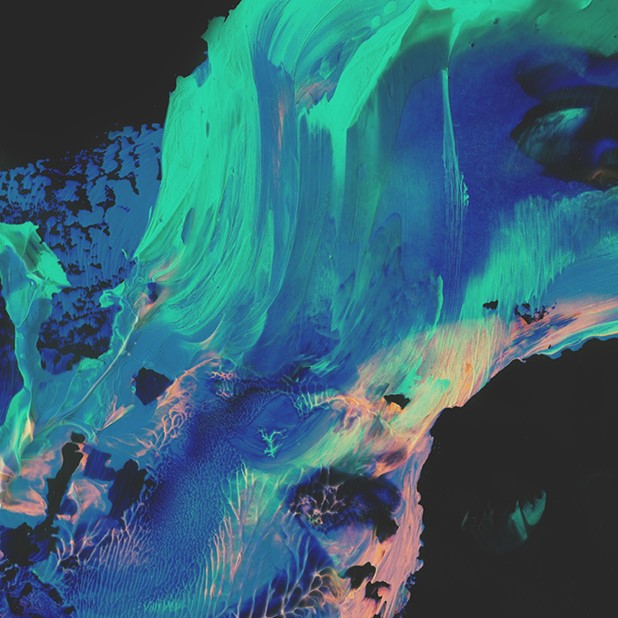
\includegraphics[width=.9\paperwidth]{Figures/Titlepage.jpg}};
        \node[anchor=south west,align=left] at (BackgroundUmu.south west) {\color{white}
            \begin{tabular}{lll}
                Supervisors & Kevin Kamm & Umeå University\\
                            & Victor Jonsson & Vermiculus Financial Technology\\
                Examiner & Christian Ewald & Umeå University
            \end{tabular}
        };
    \end{tikzpicture}
    \end{center}
\vspace*{5cm}
\begin{center}
    {%  
        \color{white}
        \noindent
        \Huge
        \bfseries 
        \sffamily
        Johans Thesis
    }\\[1em]
    {%
        \color{white}
        \noindent
        \Large
        \bfseries 
        \sffamily
        Subtitle of Thesis
    }%
\end{center}
\renewcommand{\thefootnote}{\fnsymbol{footnote}}
%\footnotetext[1]{Department of Mathematics and Statistics, Umeå University, Sweden}
\footnotetext[2]{johe6227@student.umu.se}
%\footnotetext[3]{E-mail: name.surname@umu.se}

\begin{center}
    \color{white}
    \large
    Johan Herbert%
    %\footnotemark[1]{}%\textsuperscript{,}%
    \footnotemark[2]{}
    \hspace{2em}
    % Name Surname%
    % \footnotemark[1]{}\textsuperscript{,}%
    % \footnotemark[3]{}
    \hspace{2em}
\end{center}
\begin{center}
    \color{white}
    \large
    Examination Date: \today
\end{center}
\vfill
\begin{center}
    Master thesis, 30 ECTS\\
    M.Sc in Industrial Engineering and Management, 300 ECTS\\
    Spring term 2025
\end{center}


\renewcommand{\thefootnote}{\arabic{footnote}}


\thispagestyle{empty}
\end{titlepage}
\pagenumbering{Roman}


%%%%%%%%%%%%%%%%%%%%%%%%%%%%%%%%%%%%%%%%%%%%%%%%%%%%%%%%%%%%%%%%%%%%%%%%%%%%%%%%%%%%%%%%%%%
%% Abstracts
%%%%%%%%%%%%%%%%%%%%%%%%%%%%%%%%%%%%%%%%%%%%%%%%%%%%%%%%%%%%%%%%%%%%%%%%%%%%%%%%%%%%%%%%%%%
\begin{abstract}
    This is the english abstract.

    This thesis investigates the use of copulas for modeling dependency structures between financial asset returns, with a specific focus on a recently introduced method known as the \gls{NC}. The work is carried out in collaboration with Vermiculus Financial Technology and aims to enhance risk modeling in clearing systems. Traditional copulas are compared to the \gls{NC} in terms of performance, adaptability, and applicability to different dependency structures. The study involves the development of an alternative method for fitting marginal distributions and a practical sampling approach for the \gls{NC}. Simulated data is used to evaluate the methods under controlled conditions. The results show that the \gls{NC} cannot provide competitive performance compared to other copulas in capturing complex dependencies. This work contributes to the understanding of when and how to use neural copulas in financial risk modeling.

\end{abstract}

\newpage
\renewcommand{\abstractname}{Sammanfattning}
\begin{abstract}
    Det är svenska sammanfattning.

    Denna masteruppsats undersöker användningen av copulor för att modellera beroendestrukturer mellan finansiella tillgångars avkastningar, med särskilt fokus på en nyligen introducerad metod kallad \gls{NC}. Arbetet har genomförts i samarbete med Vermiculus Financial Technology och syftar till att förbättra riskmodellering i clearingsystem. Traditionella copulor jämförs med \gls{NC} avseende prestanda, anpassningsförmåga och tillämplighet på olika typer av beroenden. Studien omfattar utvecklingen av en alternativ metod för att anpassa marginalfördelningar samt ett praktiskt tillvägagångssätt för slumptalsgenerering från \gls{NC}. Simulerad data används för att utvärdera metoderna under kontrollerade förhållanden. Resultaten visar att \gls{NC} inte producerar bättre resultat än övriga traditionella metoder vid modellering av komplexa beroenden, även om dess effektivitet är beroende av datakaraktäristik och korrekt träning. Uppsatsen bidrar till en ökad förståelse för när och hur neural copula kan användas inom finansiell riskmodellering.

\end{abstract}
\newpage
%%%%%%%%%%%%%%%%%%%%%%%%%%%%%%%%%%%%%%%%%%%%%%%%%%%%%%%%%%%%%%%%%%%%%%%%%%%%%%%%%%%%%%%%%%%
%% Acknowledgements
%%%%%%%%%%%%%%%%%%%%%%%%%%%%%%%%%%%%%%%%%%%%%%%%%%%%%%%%%%%%%%%%%%%%%%%%%%%%%%%%%%%%%%%%%%%
\section*{Acknowledgements}
I would like to express my gratitude to my supervisor Kevin Kamm, from Umeå University, who has been a great support and mentor during this thesis. His guidance, expertise, and excitement for the subject has been invaluable in challenging me during this thesis. I would also like to thank Victor Jonsson and Vermiculus Financial Technology for the opportunity to work on this project in addition to their warm welcome and support. Finally, I would like to thank my family and friends for their support during this thesis. 

Johan Herbert\\
Stockholm, Sweden\\
\today 

\newpage
%%%%%%%%%%%%%%%%%%%%%%%%%%%%%%%%%%%%%%%%%%%%%%%%%%%%%%%%%%%%%%%%%%%%%%%%%%%%%%%%%%%%%%%%%%%
%% Glossaries & Table of Contents
%%%%%%%%%%%%%%%%%%%%%%%%%%%%%%%%%%%%%%%%%%%%%%%%%%%%%%%%%%%%%%%%%%%%%%%%%%%%%%%%%%%%%%%%%%%
% \printglossary
\clearpage
\newpage
{\hypersetup{linkcolor=black}
\tableofcontents
}
\newpage
\pagenumbering{arabic}
\pagestyle{scrheadings}

%%%%%%%%%%%%%%%%%%%%%%%%%%%%%%%%%%%%%%%%%%%%%%%%%%%%%%%%%%%%%%%%%%%%%%%%%%%%%%%%%%%%%%%%%%%
%% Introduction
%%%%%%%%%%%%%%%%%%%%%%%%%%%%%%%%%%%%%%%%%%%%%%%%%%%%%%%%%%%%%%%%%%%%%%%%%%%%%%%%%%%%%%%%%%%


\section{Introduction}\label{sec:Introduction}
%%%%%%%%%%%%%%%%%%%%%%%%%%%%%%%%%%%%%%%%%%
% Revised Introduction Section
%%%%%%%%%%%%%%%%%%%%%%%%%%%%%%%%%%%%%%%%%%
We start in \Cref{AboutVFT} with providing a brief overview of the company, Vermiculus Financial Technology, and its activities. \Cref{Background} presents background information on the topic of clearing and the need for dependency modeling. \Cref{LiteratureReview} offers a brief overview of the literature and history of copulas. \Cref{Purpose} outlines the purpose, intended contributions, and research questions of this project. Finally, \Cref{Limitations} describes the limitations of this project.

\subsection{About Vermiculus Financial Technology} \label{AboutVFT}
Vermiculus Financial Technology is a software company that develops systems for financial transactions. Its three main areas of operation are trading systems, clearing systems, and \gls{CSD} systems. Trading systems match buy and sell orders in the market and determine the price at which trades are executed. Clearing systems reduce counterparty risk in financial transactions by serving as a central hub through which all transactions flow. \gls{CSD} systems track the ownership of every stock on an exchange. This project relates to the clearing segment of Vermiculus’s activities.

\subsection{Background}\label{Background}
Clearing systems exist to minimize counterparty risk in financial transactions\footnote{See "Systems in the financial infrastructure", \textit{Sveriges Riksbank}, Updated: 2024-06-28, \url{https://www.riksbank.se/en-gb/financial-stability/the-financial-system/the-financial-infrastructure/systems-in-the-financial-infrastructure/}, Last Accessed: 2025-01-29.}. Counterparty risk refers to the possibility that one party in a transaction will not fulfill its obligations, effectively defaulting on the agreement\footnote{See "Counterparty Risk", \textit{Office of the Comptroller of the Currency}, \url{https://www.occ.treas.gov/topics/supervision-and-examination/capital-markets/financial-markets/counterparty-risk/index-counterparty-risk.html}, Last Accessed: 2025-01-29.}.


A clearing house acts as an intermediary in all transactions, selling to all buyers and buying from all sellers\footnote{See Akhilesh Ganti, "Clearinghouse: An Essential Intermediary in the Financial Markets", \textit{Investopedia}, Updated: 2023-02-07, \url{https://www.investopedia.com/terms/c/clearinghouse.asp}. Last Accessed: 2025-01-27.}. Consequently, each party faces only the clearing house as its counterparty, effectively removing counterparty risk. This is illustrated in \Cref{fig:CCP} by AnalystPrep\footnote{See "Central Clearing - Financial markets and products part 1", \textit{Analyst Prep}. Updated: 2023-08-02, \url{https://analystprep.com/study-notes/frm/part-1/financial-markets-and-products/central-clearing/}, Last Accessed: 2025-01-29.}, where the right panel shows that the clearing members, marked B (usually banks), interact only with the clearing house (marked CCP). In this arrangement, as long as the clearing house remains solvent, trades can proceed even if a clearing member defaults. However, the clearing house does not provide this service for free; each party must post collateral to cover potential losses in the event of a member default. The clearing house earns revenue through fees and transaction costs, making the model viable.

In contrast, without central clearing, market participants trade directly with each other. In such a bilateral setup, both parties are exposed to counterparty risk from the time the trade is made until it is settled. For instance, the buyer might lack the funds to pay, or the seller might not possess the agreed asset. This is illustrated in the left panel of Figure~\ref{fig:CCP}, where clearing members (marked B) face each other in trades. If one member defaults, the counterparties may not receive payment, potentially triggering a chain reaction of defaults—an effect known as contagion.





\begin{figure}[ht]
    \centering
    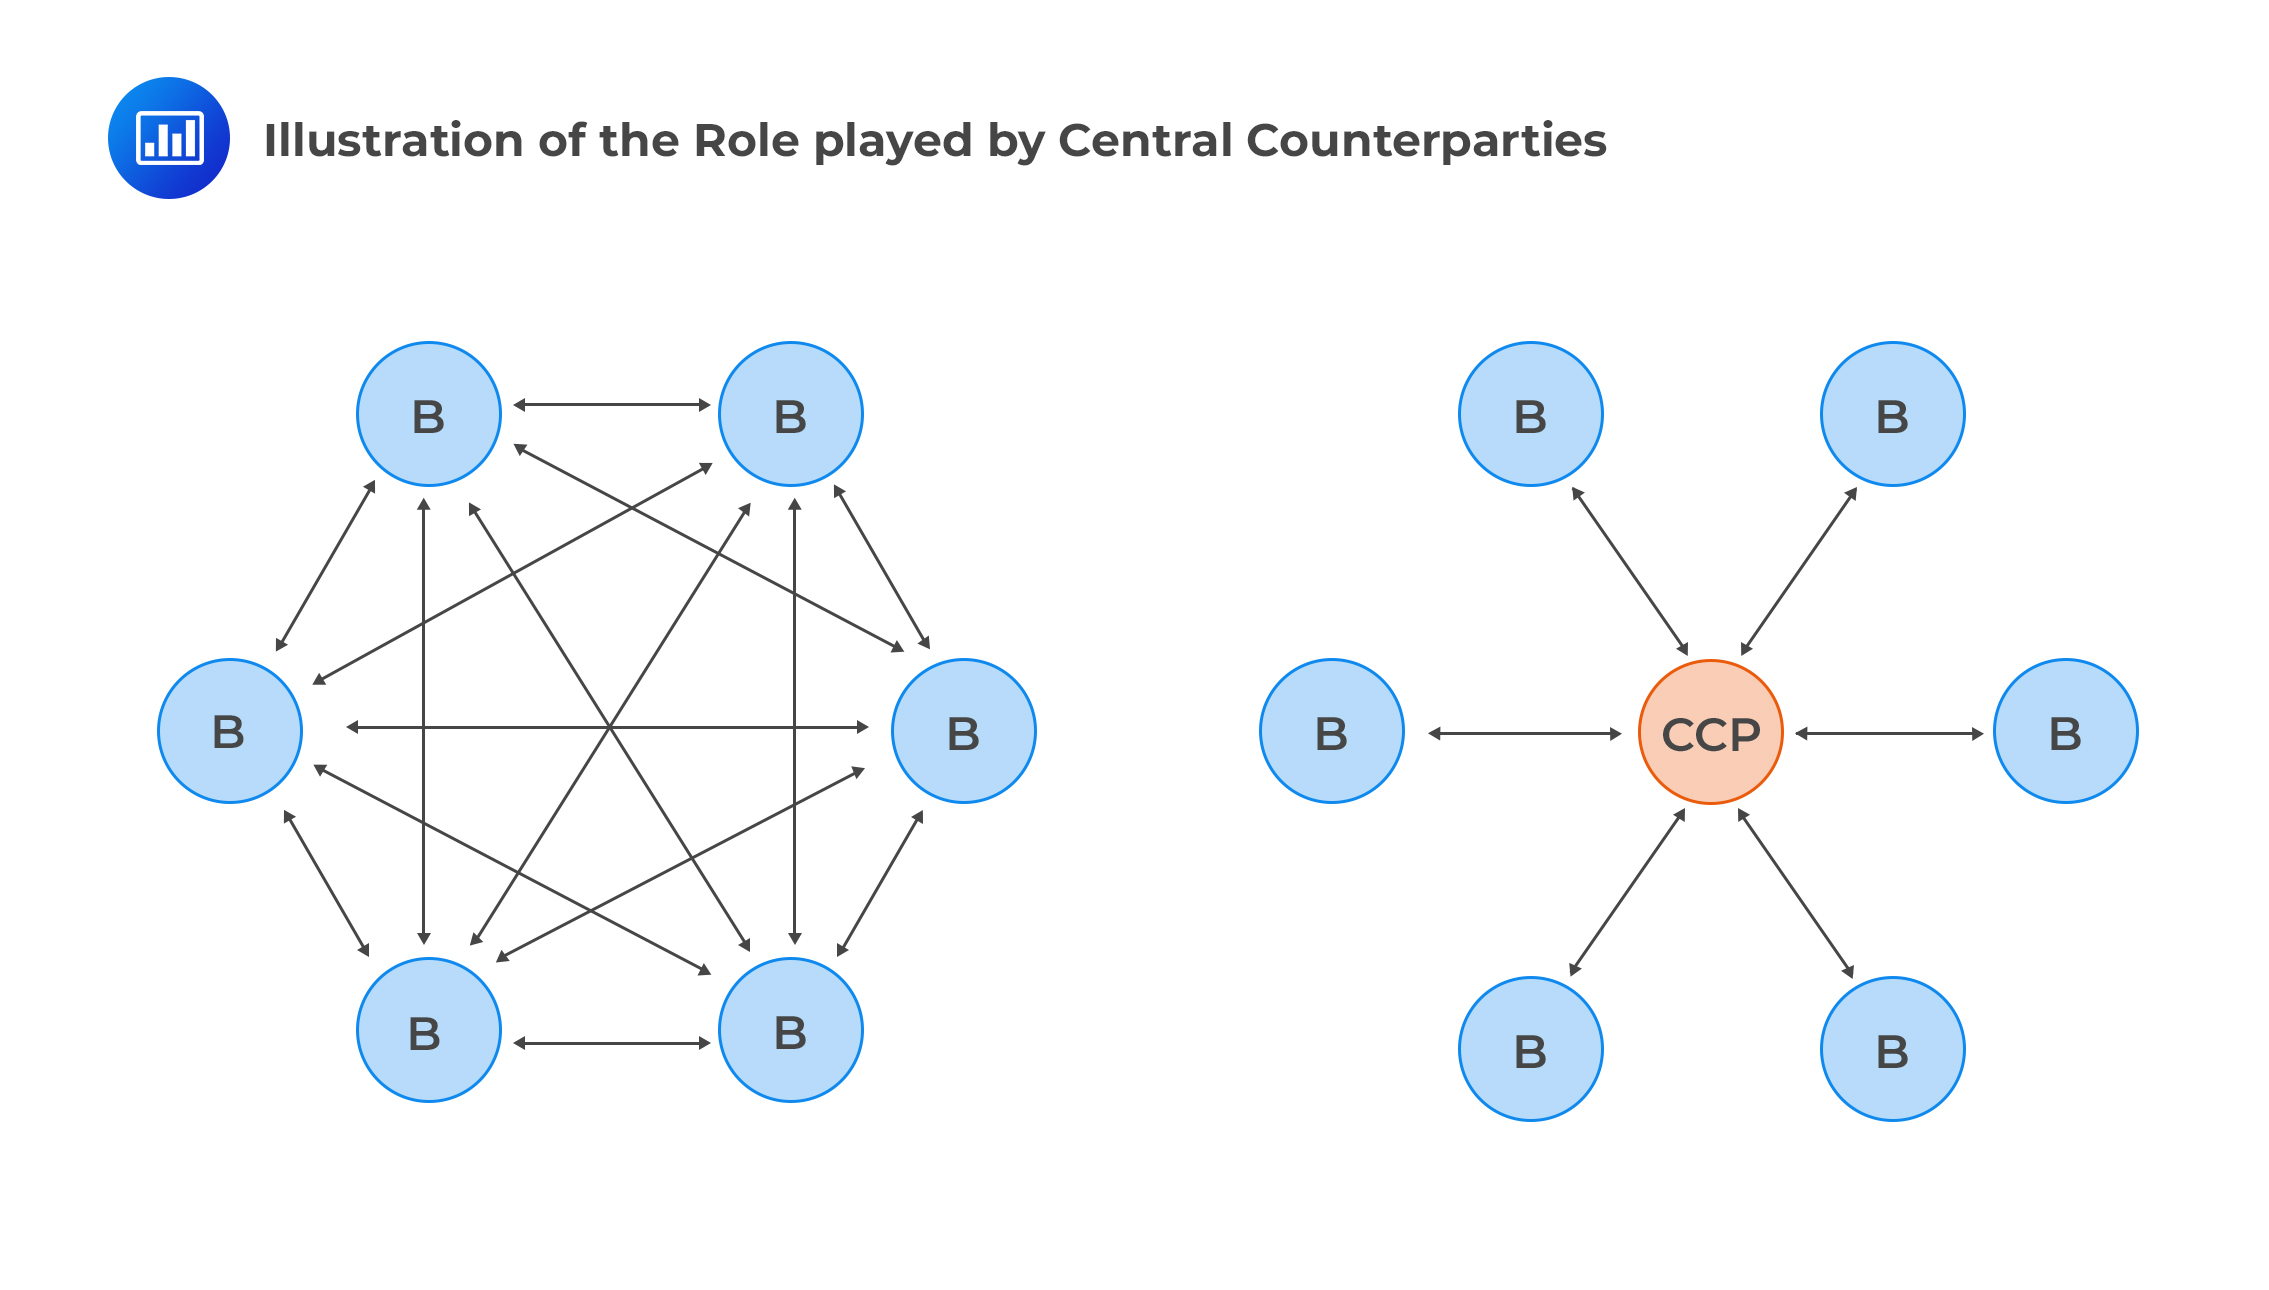
\includegraphics[width=0.7\linewidth]{1Introduction/pictures/CCPvisual .jpg}
    \caption{Bilateral and central counterparty clearing compared. The left image depicts bilateral clearing, while the right image shows central counterparty clearing. Illustration sourced from AnalystPrep\protect\footnotemark[\value{footnote}].}
    \label{fig:CCP}
\end{figure}

To determine the required collateral, the risk associated with each clearing member's portfolio must be assessed. Historically, this was done using the \gls{SPAN} framework, developed by the Chicago Mercantile Exchange\footnote{See "CME SPAN Methodology Overview", \textit{CME Group}, \url{https://www.cmegroup.com/solutions/risk-management/performance-bonds-margins/span-methodology-overview.html\#how-it-works}. Last Accessed: 2025-01-29.}. \gls{SPAN} defines various scenarios based on changes in price, volatility, and time to maturity for derivatives, and calculates the resulting changes in security values.

Following the 2008 global financial crisis, greater emphasis was placed on risk management. More recently, a shift toward using \gls{VaR} has occurred\footnote{See Rafik Mrabet, "Navigating a New Era in Derivatives Clearing", \textit{FIA}, Updated: 2024-01-04, \url{https://www.fia.org/marketvoice/articles/navigating-new-era-derivatives-clearing}. Last Accessed: 2025-01-26.}. \gls{VaR} is defined as the maximum expected portfolio loss over a specified time horizon at a given confidence level\footnote{See "Value-at-risk (VAR)", \textit{Risk.net}, \url{https://www.risk.net/definition/value-at-risk-var}. Last Accessed: 2025-01-29.}. Several methods exist for calculating \gls{VaR}, including historical, parametric, and \gls{MC} simulation approaches\footnote{See "Value-at-risk (VAR)", \textit{Corporate Finance Institute}, \url{https://corporatefinanceinstitute.com/resources/career-map/sell-side/risk-management/value-at-risk-var/}. Last Accessed: 2025-01-29.}.  

Historical \gls{VaR} uses past asset returns to compute portfolio returns at each time point. These returns are then ordered, and the \gls{VaR} is determined by selecting the percentile corresponding to the confidence level. This method realistically captures asset dependence as it is based on observed market data\footnotemark[\value{footnote}]. However, it may be inadequate due to the limited availability of extreme observations—particularly relevant for \gls{VaR}, which focuses on tail risk.

Parametric \gls{VaR} assumes that asset returns follow a known distribution. In simpler cases, the Gaussian distribution is used, with the mean vector and covariance matrix estimated from the data. This distribution is then employed to calculate the \gls{VaR} such that the probability of loss exceeding it matches the confidence level\footnotemark[\value{footnote}]. The advantage of this method lies in its simplicity and ease of use. However, it requires that the returns follow the assumed distribution, which may not always be realistic.

\gls{MC} \gls{VaR} generates artificial return scenarios by simulating random numbers from specified distributions\footnotemark[\value{footnote}]. This method is highly flexible and particularly well-suited for calculating risks associated with various types of financial instruments by simulating plausible scenarios for the portfolio’s underlying assets.

To compute \gls{MC} \gls{VaR}, the simulated returns must capture the dependence structure between assets. This can be done using covariance matrices or copulas. There are various types of copulas available, providing many modeling options—especially when fitting marginal distributions separately. This naturally leads to the purpose of this project, which follows a brief review of the literature and history of copulas.

\subsection{Literature Review and History}\label{LiteratureReview}
\Citet[pp.~1–3]{DuranteSempi2010} provide an overview of the history of copulas, which is briefly summarized here. The origins of copula theory can be traced back to Fréchet’s 1951 work on functions linking marginal and joint distributions. In 1959, Sklar introduced the term "copula" in his work on statistical metric spaces, culminating in Sklar’s theorem—a cornerstone of copula theory. About 15 years later, Schweizer began using copulas to construct dependence measures, and in 1983, Sklar and Schweizer co-authored a book on copulas. The late 1990s saw the publication of two influential books—one by Nelsen and one by Joe—which helped boost interest in copulas. As noted by Embrechts, their use in finance, particularly in models moving away from i.i.d. assumptions, contributed significantly to their rising popularity.

Despite their versatility, copulas can be difficult to apply in high-dimensional settings. In 2022, \Citet{ZengWang2022} introduced the \gls{NC}, a novel method for modeling dependence by approximating copula functions using \gls{NN}s. This approach serves as the starting point for this project.

\subsection{Purpose}\label{Purpose}
In this project we investigate various copula-based methods for modeling dependence and to clarify which methods are most appropriate for different types of data. The contributions in this thesis is to enhance understanding of how these methods can be applied in practice. In particular, the focus is on utilizing the \gls{NC} to model the dependence between log returns of different assets. To increase its practical applicability in risk management, this project explores an alternative approach to fitting marginal distributions within the \gls{NC} framework and develops a method for sampling from the \gls{NC}. 

Furthermore, the study examines which copula methods are best suited to various dependence structures and evaluates whether the \gls{NC} consistently outperforms traditional methods. Comparisons will be made between the \gls{NC} and other copulas, and strategies for training the \gls{NC} to produce reliable results will be explored. Since the \gls{NC} is a relatively new method with limited practical deployment, understanding its capabilities and limitations is essential.

The research questions guiding this project are as follows:
\begin{compactenum}[{\bfseries RQ}1]
    \item \label{item:RQ1} Is the marginal distribution used in the \gls{NC} adequate?
    \item \label{item:RQ2} How should the neural copula function be trained to yield consistently reliable results?
    \item \label{item:RQ3} Can a neural copula more accurately model the dependence between asset returns than other copula methods?
\end{compactenum}
\newcommand{\RQone}{{\bfseries RQ}\ref{item:RQ1} }
\newcommand{\RQtwo}{{\bfseries RQ}\ref{item:RQ2} }
\newcommand{\RQthree}{{\bfseries RQ}\ref{item:RQ3} }

\subsection{Limitations}\label{Limitations}
To define the scope of this project, several limitations were established during its initial phase:

\begin{compactenum}
    \item A selected subset of traditional copulas was chosen for comparison with the \gls{NC}.
    \item The portfolios analyzed will be limited to two assets to enhance interpretability and enable visualization.
    \item Artificially simulated data will be used to control the dependence between assets and to ensure consistent evaluation across methods. This also allows control over the marginal distributions, focusing the evaluation solely on the copula methods.
    \item The main emphasis of this report is the implementation and evaluation of the \gls{NC}. Once this is accomplished, additional performance measures will be considered.
\end{compactenum}

Additional limitations were introduced during the project to maintain feasibility, such as restricting the number of datasets and hyperparameters tested.

This thesis is structured as follows: \Cref{sec:theory} introduces the theoretical background necessary to understand the methods used. \Cref{sec:Method} outlines the methodology. \Cref{sec:Results} presents and discusses the results of the conducted tests. Finally, \Cref{sec:Conclusion} summarizes the findings and suggests avenues for future research.




% %%%%%%%%%%%%%%%%%%%%%%%%%%%%%%%%%%%%%%%%%%
% % Old from before fixing using chatgpt
% %%%%%%%%%%%%%%%%%%%%%%%%%%%%%%%%%%%%%%%%%%
% This section introduces the project and its purpose. \Cref{AboutVFT} will give a brief overview of the company, Vermiculus Financial Technology, and its activities. \Cref{Background} will give a background to the topic of clearing and the need for dependency modeling. \Cref{LiteratureReview} will give a brief overview of the literature  and history of copulas. \Cref{Purpose} will present the purpose, intended contributions, and research questions of this project. Finally, \Cref{Limitations} will present the limitations of this project. Finally, \Cref{Limitations} will present the limitations of this project.

% \subsection{About Vermiculus Financial Technology} \label{AboutVFT}
% Vermiculus Financial Technology is a software company that builds systems for financial transactions. Its three main areas of operations are trading systems, clearing systems, and \gls{CSD} systems. Trading systems match buy and sell orders in the market and find the price at which trades should be executed. Clearing systems reduce counterparty risk in financial transactions by acting as the central hub through which all transactions flow. \gls{CSD} systems keep track of who owns every stock on an exchange. This project will be related to the clearing section of Vermiculus activities. 

% \subsection{Background}\label{Background}
% Clearing systems are in place to minimize counterparty risk in financial transactions\footnote{See \url{https://www.riksbank.se/en-gb/financial-stability/the-financial-system/the-financial-infrastructure/systems-in-the-financial-infrastructure/}. Last Accessed: 2025-01-29}. Counterparty risk is the risk of having the other party in a transaction not fulfilling its end of a deal and hence defaulting on its obligations\footnote{See \url{https://www.occ.treas.gov/topics/supervision-and-examination/capital-markets/financial-markets/counterparty-risk/index-counterparty-risk.html}. Last Accessed: 2025-01-29}. 
% The clearing house acts as a middleman in all transactions, selling to all buyers and buying from all sellers\footnote{See \url{https://www.investopedia.com/terms/c/clearinghouse.asp}. Last Accessed: 2025-01-27}. Hence, each party only faces the clearing house as their counterparty, removing the counterparty risk, this has been nicely illustrated\footnote{See \url{https://analystprep.com/study-notes/frm/part-1/financial-markets-and-products/central-clearing/}. Last Accessed: 2025-01-29}. In the right part of Figure~\ref{fig:CCP} we can see the clearing members marked B, usually banks, that only face the clearing house marked CCP. In this system, as long as the clearing house does not go bankrupt, trades can go through even if a clearing member defaults on their commitment. The clearing house does not offer this risk removal for free; rather, it requires each party to post collateral covering the costs if a clearing member defaults. The clearinghouse makes money from fees and transaction costs, making it worthwhile.

% The alternative to centrally cleared trading is that each market participant trades directly with each other. In this case, both sides of a transaction are exposed to counterparty risk from when making a trade until it has been settled. The risk in this scenario is that the buyer does not have enough money to pay or that the seller does not have the asset it has agreed to sell. This is nicely illustrated\footnotemark[\value{footnote}] in the left part of Figure \ref{fig:CCP}. We can see that each clearing member, marked B, faces each other if having the buy and sell side of the same position. In this system, if one of the clearing members defaults, it can impact the other clearing members, who will not get their money. This can cause contagion, so if one clearing member goes bankrupt, others may follow suit. 

% \begin{figure}[ht]
%     \centering
%     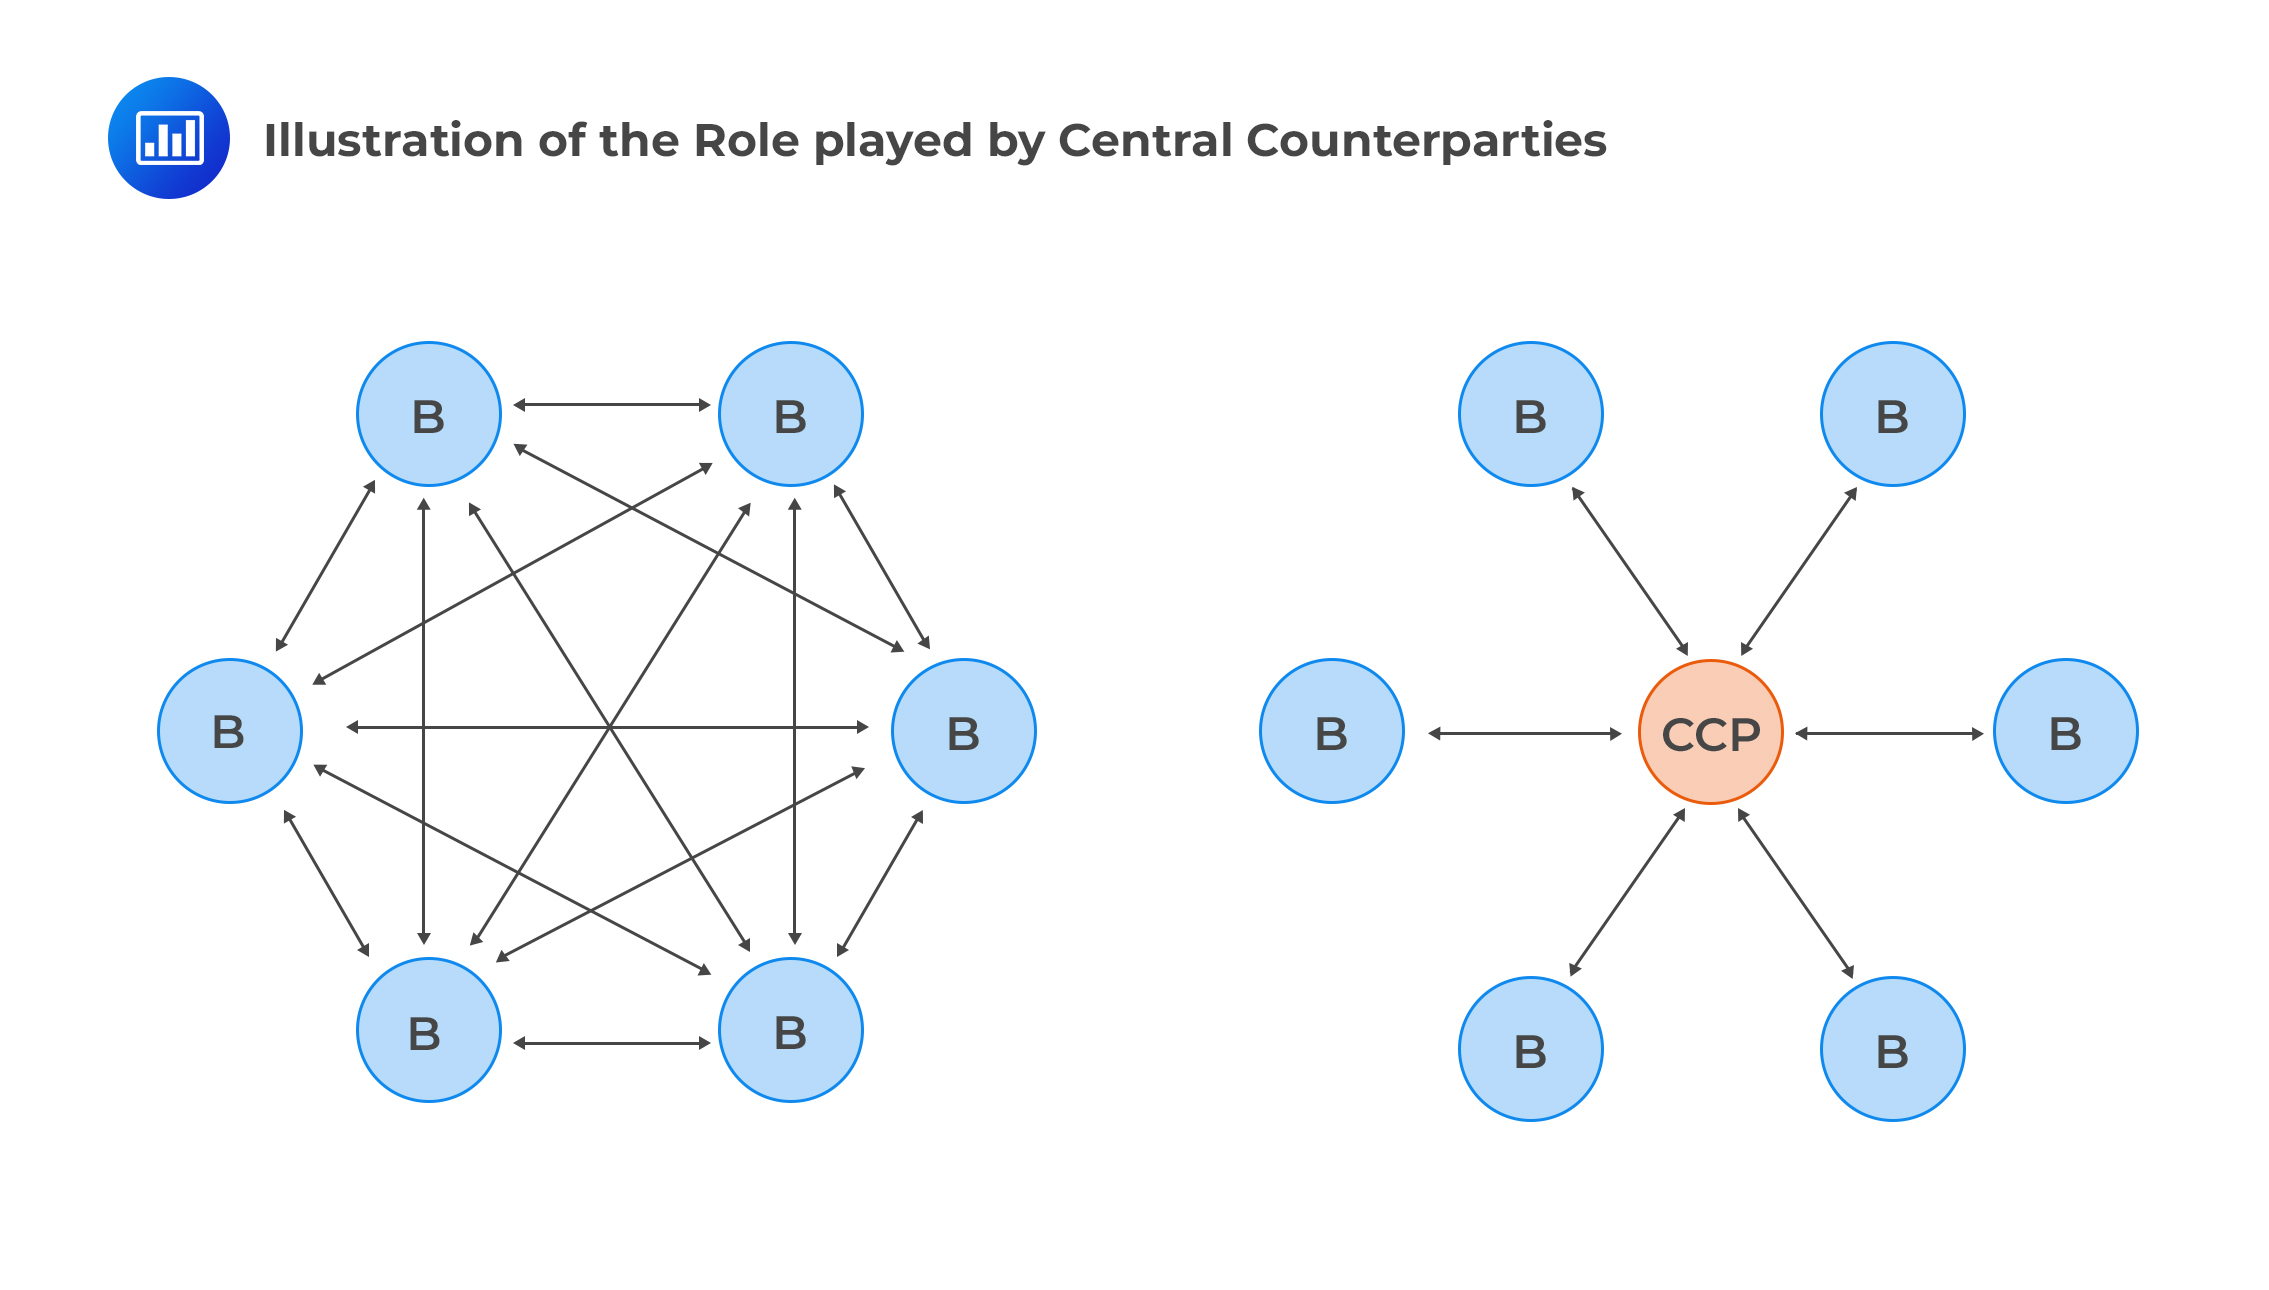
\includegraphics[width=0.7\linewidth]{1Introduction/pictures/CCPvisual .jpg}
%     \caption{Bilateral and central counterparty clearing compared. The left picture shows a system of parties that are clearing transactions bilaterally. The right picture shows a system where central counterparty clearing is used. This illustration was found at AnalystPrep\protect\footnotemark[\value{footnote}]. }
%     \label{fig:CCP}
% \end{figure}

% To determine how much collateral is required from each clearing member, the risk of its portfolio must be measured. Historically this has been done using a framework called \gls{SPAN} that was developed by Chicago Mercantile Exchange\footnote{See \url{https://www.cmegroup.com/solutions/risk-management/performance-bonds-margins/span-methodology-overview.html\#how-it-works}.  Last Accessed: 2025-01-29}. The \gls{SPAN} framework has several scenarios based on changes in price, volatility, and time to maturity for derivatives. These scenarios are then used to calculate what change in value they would have for some security. Since the global financial crisis in 2008, more focus has been put on risk management. In later years a shift towards using \gls{VaR} has taken place\footnote{See \url{https://www.fia.org/marketvoice/articles/navigating-new-era-derivatives-clearing}. Last Accessed: 2025-01-26}. \gls{VaR} is a measure defined as the maximum expected loss in portfolio value over a time horizon for some level of confidence\footnote{See \url{https://www.risk.net/definition/value-at-risk-var}. Last Accessed: 2025-01-29}. There are several ways of calculating value at risk \gls{VaR} such as historical, parametric, and \gls{MC} simulated among others \footnote{See \url{https://corporatefinanceinstitute.com/resources/career-map/sell-side/risk-management/value-at-risk-var/}. Last Accessed: 2025-01-29}.  

% Historical \gls{VaR} uses historical returns from the different assets in it to calculate the return of the portfolio at each time step. These portfolio returns are then ordered and the percentile corresponding to the confidence level is calculated giving the \gls{VaR}. This method has advantages and disadvantages. The advantage is that the dependence between assets is completely realistic as it comes from the true observations on the market\footnotemark[\value{footnote}]. A disadvantage is however that this model can be insufficient because the observations from the data are limited. This might sound strange but when observations falling in the tails of a distribution is of course rare. This means that for \gls{VaR}, which focuses on the lower tail, the amount of data available might not be enough to precisely determine the \gls{VaR}.  

% Parametric \gls{VaR} assumes that the returns for an asset are generated from some distribution. These returns are then used for calculating the described characteristics of the distribution. In simple \gls{VaR} models, the Gaussian distribution is often used, in which case the mean vector and covariance matrix are estimated. This distribution is then used to calculate the \gls{VaR} so that the probability of ending up below the limit aligns with the confidence\footnotemark[\value{footnote}]. This method has the advantage that it is easy to use and understand. It has a disadvantage in that it requires the data to follow some known distribution which might not always be a realistic assumption.  

% \gls{MC} \gls{VaR} utilizes simulated random numbers to generate artificial return scenarios from which the \gls{VaR} can be calculated\footnotemark[\value{footnote}]. \gls{MC} simulations have a major advantage over the other methods mentioned in that they can be used for calculating the risks of different types of financial instruments. This is done by simulating plausible scenarios for the underlying assets of a portfolio.  

% The returns used for computing \gls{MC} \gls{VaR} need to be simulated from distributions with dependence that reflect how different assets move in relation to one another. Several methods can be used to do this, such as using covariance matrices or copulas. There are several different types of copulas to use, meaning that there are many alternative methods to choose from, especially when also having the task of fitting marginal distributions to the data. This leads us to the purpose of this project, but first, a brief overview of the literature and history of copulas will be given.

% \subsection{Literature review and history}\label{LiteratureReview}
% \Citet[pp.~1-3]{DuranteSempi2010} provides an overview of the history of copulas. In this paragraph, a brief summary of their overview will be given. It is possible to mark the starting point of the copula theory to the work of Fréchet in 1951, studying the class of functions linking marginal distributions to joint distributions. In 1959 Sklar introduced the term copula in his work on statistical metric spaces. This resulted in Sklar's theorem which is central to the theory of copulas. Roughly 15 years later Schweizer introduced the use of copulas to construct dependence measures. In 1983 Sklar and Schweizer published  a book on copulas. During the late 1990s two books on copulas were published, one by Nelsen and one by Joe. The interest in copulas increased significantly due to applications in finance as said by Embrechts. Particularly, the move from models using i.i.d. assumptions was contributing to the increased interest in copulas. 

% A challenge with copulas is that they are not always easy to use, particularly when the dimensionality of the data increases. In 2022 \Citet{ZengWang2022} introduced the \gls{NC} which is a new method of modeling dependence by approximating a copula function using \gls{NN}s. This method will be the starting point of this project. 


% % Copulas are widely used in mathematical finance \Citet[p.~1]{Umberto2004copulaMethods}. The use cases are many but some of the most common are pricing of basket options \Citet[pp.~279-280]{Umberto2004copulaMethods}, \gls{VaR} \Citet[p.~253]{Alexander2008} calculations, and credit risk \Citet[p.~1]{Umberto2004copulaMethods}. It is particularly useful because it allows for modeling dependence separate from the marginal distributions which is useful when returns are not both normally or students $t$ distributed \Citet[p.~253]{Alexander2008}. 
% % \todo{Reference to the summary article on copulas. Remove the connection to mathematical finance.}


 
% \subsection{Purpose}\label{Purpose}
% The purpose of this project is to investigate different copula methods of modeling dependence and to provide clarity about which method to use for what type of data. The intended contribution of this project is to provide a better understanding of how different methods of modeling dependence can be used in practice. More specifically, the focus will be on how to use the \gls{NC} to model dependence between log returns of different assets. To make the \gls{NC} method more useful in practical risk applications, an alternative method for fitting the \gls{NC} marginal distributions will be investigated. Additionally, an approach for sampling the \gls{NC} will be developed to make it useful in practice. Finally, we will investigate what copula method to use when and investigate if the \gls{NC} outperforms other methods for all types of dependence structures. This will be done by comparing the \gls{NC} to other copula methods and by investigating how the \gls{NC} can be trained to obtain reliable results. The \gls{NC} is a new method that has not been widely used in practice yet, so it is important to understand how it can be used and what its limitations are. 

% The research questions that will be studied in this project are introduced below:
% %\paragraph*{Research questions.}
% \begin{compactenum}[{\bfseries RQ}1]
%     \item \label{item:RQ1} Is the marginal distribution used in the \gls{NC} adequate to use?
%     \item \label{item:RQ2} How should the neural copula function be trained to obtain consistently reliable results?
%     \item \label{item:RQ3} Can a neural copula be used to better model the dependence between asset returns than other copulas?
% \end{compactenum}
% \newcommand{\RQone}{{\bfseries RQ}\ref{item:RQ1} }
% \newcommand{\RQtwo}{{\bfseries RQ}\ref{item:RQ2} }
% \newcommand{\RQthree}{{\bfseries RQ}\ref{item:RQ3} }

% \subsection{Limitations}\label{Limitations}
% To restrict the scope of this project some limitations was determined during the initial phase of the project.

% \begin{compactenum}
%     \item A selection of traditional copulas to compare the \gls{NC} to was made. 
%     \item The number of assets in the portfolios will be limited to two assets. This will help with interpretability as it allows for visualization. 
%     \item The data used will be artificially simulated to control the dependence between the assets in the portfolios and to be able to evaluate each method under consistent conditions. This also allows us to control the marginal distributions of the data, making the test only focus on the copula methods.  
%     \item The main focus of this report is to implement and evaluate the \gls{NC}. When this is done, other measures will be considered. 
% \end{compactenum}
% Additional limitations have been made along the way to make the project more manageable. For example, the number of datasets tested, and the number of hyper parameters tested.  

% This thesis is structured as follows: \Cref{sec:theory} will give an introduction to the theory, necessary for understanding the methods used in this project. \Cref{sec:Method} will present the methods used in this project. \Cref{sec:Results} will present and discuss the results of the tests conducted. Finally, \Cref{sec:Conclusion} will summarize the findings and suggest future work. 






% %%%%%%%%%%%%%%%%%%%%%%%%%%%%%%%%%%%%%%%%%%%%%%%%%%%%%%%%%%%%%%%%%%%%%%%%%%%%%%%%%%%%%%%%%%%
% %% Background
% %%%%%%%%%%%%%%%%%%%%%%%%%%%%%%%%%%%%%%%%%%%%%%%%%%%%%%%%%%%%%%%%%%%%%%%%%%%%%%%%%%%%%%%%%%%
% \section{Background}\label{sec:Background}
% 





%%%%%%%%%%%%%%%%%%%%%%%%%%%%%%%%%%%%%%%%%%%%%%%%%%%%%%%%%%%%%%%%%%%%%%%%%%%%%%%%%%%%%%%%%%%
%% Theory
%%%%%%%%%%%%%%%%%%%%%%%%%%%%%%%%%%%%%%%%%%%%%%%%%%%%%%%%%%%%%%%%%%%%%%%%%%%%%%%%%%%%%%%%%%%
\section{Theory}\label{sec:theory}
% \begin{generalinstructions}
% Make sure the notation is consistent, Predefine $\bar{R},I $ for example. Also, look over and rewrite theorems so that they fit together with the notation. Ensure consistency in number of dimensions.
% \end{generalinstructions}


%%%%%%%%%%%%%%%%%%%%%%%%%%%%%%%%%%%%%%%%%%%%%%%%%%%%%%%%%%%%%%%%%%%%%%%%%%%%%%%%%%%%%%%%%%%%%%
%%%%%%%% Mathematical finance
%%%%%%%%%%%%%%%%%%%%%%%%%%%%%%%%%%%%%%%%%%%%%%%%%%%%%%%%%%%%%%%%%%%%%%%%%%%%%%%%%%%%%%%%%%%%%%
\subsection{Mathematical finance}\label{sec:MathematicalFinance}
%\todo{What is Mathematical finance}
In mathematical finance, one is typically interested in the returns of financial assets, over discrete time steps, rather than their price \citet[p.~2]{Danielsson2011}. Let $P_{t_i}$ denote the price at time increment $t_i$, where $t_i$ is usually in daily time increments, but can be any unit of time. 


\subsubsection{Returns}
This section will introduce different types of returns, simple and log, as well as their different properties. These properties are for example return aggregation over time, portfolio return calculations, generation of new prices, and the bounds for returns. The reason for introducing different types of returns is to show the connections between financial returns and statistical distributions that in turn connect to the theory of copulas. 

Firstly we should introduce what financial returns on assets are. The return of a financial asset is the relative price change over a given time interval, often expressed as a percentage \citet[p.~2]{Danielsson2011}. One type of return is simple returns, defined in \Cref{def:simpleReturns}.

\begin{definition}\label{def:simpleReturns}
    \textbf{Simple-Returns} \citet[p.~3]{Danielsson2011}
    A \emph{simple return} is the percentage change in price, over time period $t_i$, indicated by $R_{t_i}$:
    \begin{align*}
        R_{t_i} = \frac{P_{t_i}-P_{t_{i-1}}}{P_{t_{i-1}}}.
    \end{align*}
\end{definition}

To aggregate several simple (daily) returns over some time (week) to the return over the whole period (week), one has to construct several change factors that are multiplied together before subtracting one. This aggregation process is described in \citet[p.~3]{Danielsson2011}, where the aggregated return over $n$ periods can be calculated as
\begin{align*}
    R_{t_{i}}(n) = (1+R_{t_{i}})(1+R_{t_{i-1}})(1+R_{t_{i-2}})\dots (1+R_{t_{i-n+1}}) -1 = \frac{P_{t_{i}}}{P_{t_{i-n}}}-1.
\end{align*}

In many situations, it is necessary to calculate the return of an entire portfolio of assets from its underlying asset returns. For simple returns, this is simply done by calculating a weighted average of the individual asset returns. \citet[p.~3]{Danielsson2011} describes the calculation of the portfolio return $R_{t_i,\mathrm{port}}$ for a portfolio with $K$ different assets as 
\begin{align*}
    R_{t,\mathrm{port}} = \sum_{k=1}^K w_kR_{t,k}.
\end{align*}

Many times, it can be useful to simulate new stock prices by using randomly generated returns. For simple returns, new prices can be calculated as
\begin{align*}
    P_{t_{i}} = P_{t_{i-1}}(1+R_{t_{i}}).
\end{align*}

The space in which realizations of returns can be observed differs for different types of returns. In \Cref{ex:BoundsSimpleReturns} the range for simple returns is derived. 

\begin{example}\label{ex:BoundsSimpleReturns}
    To see the bounds for simple returns, we investigate what happens as the stock price moves to zero, corresponding to bankruptcy, and when the stock price moves to infinity. We denote the simple return when the price goes to zero and infinity by $R_t^-$ and $R_t^+$ respectively   
    \begin{align*}
        R_{t_i}^- = \lim_{P_{t_i} \to 0} \frac{P_{t_i}-P_{t_{i-1}}}{P_{t_{i-1}}} = \frac{0-P_{t_{i-1}}}{P_{t_{i-1}}} =  -1 \\
        R_{t_i}^+ =\lim_{P_{t_i} \to \infty} \frac{P_{t_i}-P_{t_{i-1}}}{P_{t_{i-1}}} = \frac{\infty-P_{t_{i-1}}}{P_{t_{i-1}}}=\infty.\\    
    \end{align*}
Hence, we conclude that $R_t \in (R_t^-,R_t^+) = [-1,\infty)$. 
\end{example}


Continuously compounded returns or so-called logarithmic returns are often used for financial modeling given their desirable properties. A desirable property is that the returns are \emph{symmetric}, so positive and negative returns of the same magnitude cancel each other out \citet[p.~4]{Danielsson2011}. Log returns are defined, as done by \citet[p.~3]{Danielsson2011}, in \Cref{def:logReturns}. 

\begin{definition}\label{def:logReturns}
    \textbf{Log-Returns} \\
    The logarithm of gross return or \emph{log-returns}, indicated by $Y_{t_i}$:
    \begin{align*}
        Y_{t_i} = \mathrm{log}(1+R_{t_i}) = \mathrm{log} \left(\frac{P_{t_i}}{P_{t_{i-1}}}\right) = \mathrm{log}(P_{t_{i}}) -\mathrm{log}(P_{t_{i-1}})
    \end{align*}
\end{definition}

Log-returns have the advantage that the multiperiod, $n$ period, returns are just the sum of one period returns \citet[p.~3]{Danielsson2011}, that is 
\begin{align*}
    Y_{t_i}(n) = Y_{t_i}+Y_{t_{i-1}} + \dots + Y_{t_{i-n+1}}.
\end{align*}

 
As illustrated by \citet[p.~4]{Danielsson2011}, the portfolio return is more complicated to compute for log returns because the relation is not simply a weighted sum
\begin{align*}
        Y_{t_i,\mathrm{port}} &= \mathrm{log}\left(\frac{P_{t_i,\mathrm{port}}}{P_{t_{i-1},\mathrm{port}}}\right) \neq  \sum_{k=1}^K w_k\mathrm{log}\left(\frac{P_{t_i,k}}{P_{t_{i-1},k}}\right), \mathrm{where} \;\\
        P_{t_i,\mathrm{port}} &= \sum_{k=1}^K w_k P_{t_i,k}.
\end{align*}


A weighted average is approximately, but not quite correctly, describing the portfolio returns in terms of the individual returns as described by \citet[p.~3]{Danielsson2011},
\begin{align*}
    Y_{t_i,\mathrm{port}} \approx \sum_{k=1}^K w_k R_{t_i,k}.
\end{align*}

The correct relation between portfolio log returns and its sub-components log returns is given by first converting the log returns to prices, then calculating the portfolio returns before calculating the log return from the portfolio return
\begin{align*}
    Y_{t_i,\mathrm{port}} = \mathrm{log} \left( \frac{\sum_{k=1}^K w_k P_{t_i,k}}{\sum_{k=1}^K w_k P_{t_{i-1},k}}\right), \mathrm{where} \; P_{t_i,k} = P_{t_i-1,k}e^{Y_{t_i,k}}.
\end{align*}
In the above expression, the nominator represents the new portfolio value while the denominator represents the initial portfolio value. $K\in \mathbb{N}$ is the number of assets in the portfolio and $w_k$ is the weight of the total portfolio in asset $k$. Note that the individual asset prices are updated, using the log return, by themselves before weighing them together as a portfolio value. 

In many applications, one wants to simulate returns to produce artificial stock price developments. Log returns from stock prices usually seem to be generated from some sort of bell-shaped probability distribution. This makes it convenient becausecause one can use samples from some probability distribution as the log returns when simulating prices for an asset. As an example, the famous Black-Scholes model assumes that stock returns are log normally distributed. That is, the log returns are normally distributed. 

%\todo{what to do with t here?}
To obtain the price $P_{t_i}$ at the end of time period $t_i$ using a simulated log return $Y_{t_i}$ for period $t_i$, one can calculate 
\begin{align*}
    P_{t_i} = P_{t_{i-1}}e^{Y_{t_i}}. %(own)
\end{align*}

The range in which log returns can be observed is, unlike those in the simple return case, unbounded both positively and negatively. 
\begin{example}
    To see this we investigate what happens to the returns when the stock price moves to zero, corresponding to bankruptcy, and when the stock price moves to infinity. We denote the log return when the price goes to zero and infinity by $Y_t^-$ and $Y_t^+$ respectively.   
    \begin{align*}
        Y_{t_i}^- = \lim_{P_{t_i} \to 0} \mathrm{log} \left( \frac{P_{t_i}}{P_{t_{i-1}}}\right) = \mathrm{log}(0)= -\infty\\
        Y_{t_i}^+ =\lim_{P_{t_i} \to \infty} \mathrm{log}\left( \frac{P_{t_i}}{P_{t_{i-1}}}\right) = \mathrm{log}(\infty)= \infty\\    
    \end{align*}
    Hence, we conclude that $Y_{t_i} \in (Y_{t_i}^-,Y_{t_i}^+) = (-\infty,\infty)$. 
\end{example}

To better understand how the different types of returns work, \Cref{ex:returnSymmetry} shows that simple returns are not symmetrical whereas log returns are. 
\begin{example}\label{ex:returnSymmetry}
    \textbf{Symmetry of returns} (own example, on the same lines as \citet[p.~4]{Danielsson2011} but not quite)
    Consider an example of a stock having initial price $P_0 = 100$, price after one day $P_1 = 200$, and price at day two $P_2 = 100$. Let's examine what these price changes do to simple and log returns respectively.
    
    \textbf{Simple returns}\\
    The return on the first day is
    \begin{align*}
        R_1 = \frac{P_1-P_0}{P_0} = \frac{200-100}{100} = 1 = 100\%.
    \end{align*}
    The return on the second day is
    \begin{align*}
        R_2 = \frac{P_2-P_1}{P_1} = \frac{100-200}{200} = -\frac{1}{2} = -50\%.
    \end{align*}    
    \textbf{Log returns}\\
    The return on the first day is 
    \begin{align*}
       Y_1 = \log \left( \frac{P_1}{P_0}\right) = \log\left(\frac{200}{100}\right)  = \log(2) \approx 69 \%.
    \end{align*}
    The return on the second day is
    \begin{align*}
        Y_2 = \log\left(\frac{P_2}{P_1}\right) = \log\left(\frac{100}{200}\right)= \log\left(\frac{1}{2}\right) \approx -69\%.
    \end{align*}
    We can see that the log returns are symmetrical so that monetary gains and losses of equal magnitude have log returns of equal magnitude. This is in contrast to simple returns where gains and losses are not symmetrical.
\end{example}



%%%%%%%%%%%%%%%%%%%%%%%%%%%%%%%%%%%%%%%%%%%%%%%%%%%%%%%%%%%%%%%%%%%%%%%%%%%%
%%%% GBM
%%%%%%%%%%%%%%%%%%%%%%%%%%%%%%%%%%%%%%%%%%%%%%%%%%%%%%%%%%%%%%%%%%%%%%%%%%%%
\subsubsection{Geometric Brownian motion}
The symmetrical property of log returns is desirable because it means that the log returns can be modeled using a normal distribution. This is a convenient because the normal distribution has many nice properties and is easy to work with. Log returns are often used in financial modeling, perhaps most notably in the Black-Scholes model, for option pricing, where stock prices are assumed to follow a \gls{GBM} which price is log normally distributed. This is a consequence of the log returns being normally distributed. The \gls{GBM} is a stochastic process that is used to model the evolution of stock prices. The \gls{GBM} is defined by the stochastic differential equation (SDE)
\begin{align*}
    dS_t &= \mu S_t dt + \sigma S_t dW_t \\
    S_0 &= s_0, 
\end{align*}
where $S_t$ is the stock price at time $t$, $\mu$ is the drift, $\sigma$ is the volatility, and $W_t$ is a Wiener process \Citet[p.~67]{Bjork2019Edition4} \todo{Find page where GBM defined}. The \gls{GBM} can be solved using the Itô formula, which gives the solution
\begin{align*}
    S_t = s_0 \;\mathrm{exp}\left( \left( \mu - \frac{\sigma^2}{2} \right)t + \sigma W_t \right),
\end{align*}
\Citet[p.~70]{Bjork2019Edition4}.

%%%%%%%%%%%%%%%%%%%%%%%%%%%%%%%%%%%%%%%%%%%%%%%%%%%%%%%%%%%%%%%%%%%%%%%%%%%%
%%%% Euler Maruyama
%%%%%%%%%%%%%%%%%%%%%%%%%%%%%%%%%%%%%%%%%%%%%%%%%%%%%%%%%%%%%%%%%%%%%%%%%%%%
\subsubsection{Euler-Maruyama Scheme}\label{sec:EulerMaruyama}
To approximately simulate \gls{SDE}s the Euler-Maruyama scheme can be used. The Euler-Maruyama scheme is a numerical method for solving \gls{SDE}s. 

For an \gls{SDE} of the form
\begin{align*}
    dX_t = a(X_t)dt + b(X_t)dW_t,
\end{align*}
the Euler-Maruyama scheme is defined as follows. 
Let $\hat{X}$ denote the approximate solution to the \gls{SDE} and let $X$ denote the exact solution. The Euler-Maruyama scheme is defined by the following recursive formula 
\begin{align*}
    \hat{X}(t_{i+1}) = \hat{X}(t_i) + a(\hat{X}(t_i))[t_{i+1}-t_i]  + b(\hat{X}(t_i)) \sqrt{t_{i+1}-t_i} Z_{i+1},
\end{align*}
where $Z_{i+1}$ is a standard normal random variable. The time step $t_{i+1}-t_i$ is the time increment, and $a$ and $b$ are the drift and diffusion functions respectively \Citet[pp.~339-340]{glasserman2004monte}.

We can use the Euler-Maruyama scheme to simulate a stock trajectory with the \gls{GBM} by setting $a(S_t) = \mu S_t$ and $b(S_t) = \sigma S_t$. The resulting scheme is
\begin{align*}
    \hat{S}(t_{i+1}) = \hat{S}(t_i) + \mu \hat{S}(t_i)[t_{i+1}-t_i]  + \sigma \hat{S}(t_i) \sqrt{t_{i+1}-t_i} Z_{i+1}.
\end{align*}
To simulate a stock trajectory, the time increment $t_{i+1}-t_i$ is set to a small value, and the process is iterated for a large number of steps. 

We can simulate a pair of dependent stock trajectroies by simulating a system of \gls{GBM}s  
\begin{align*}
    dS_t^d = \mu S_t^d dt + \sigma S_t^d dW_t^d, \; d=1,2, 
\end{align*}
where $W_t^1$ and $W_t^2$ are standard one dimensional Wiener processes with correlation $\rho$ \Citet[p.~104]{glasserman2004monte}. One can also simulate a system of \gls{GBM}s with a dependence different than correlation. This can be done by using a copula to generate the dependent Weiner processes.

In financial applications one is often interested in what impact changes in asset prices have on the value of a financial instrument and risk metrics. To do this a widely used method is to simulate the future price of the underlying asset and then calculate how the value of the instrument or metric changes based on the simulated prices. This allows for the calculation of risk metrics such as \gls{VaR} and \gls{ES} as well as the pricing of financial instruments such as options. The method is often referred to as Monte Carlo simulation.  

%%%%%%%%%%%%%%%%%%%%%%%%%%%%%%%%%%%%%%%%%%%%%%%%%%%%%%%%%%%%%%%%%%%%%%%%%%%%
%%%% Monte Carlo methods
%%%%%%%%%%%%%%%%%%%%%%%%%%%%%%%%%%%%%%%%%%%%%%%%%%%%%%%%%%%%%%%%%%%%%%%%%%%%
\subsubsection{Monte Carlo methods} \label{sec:MonteCarlo}
% \begin{generalinstructions}
%     \textbf{I would say}\\
%     Monte Carlo methods is a blanket term for computational methods that utilize random numbers to model uncertain events. Given an assumption about the underlying distribution of a random process. The random process is simulated multiple times and used as the input in a deterministic function, the result of which is averaged. 
% \end{generalinstructions}
Many times in different scientific fields, relationships between different variables can be described using deterministic relationships between input variables and output variables. In some situations, these deterministic relationships have random input parameters. In these cases, Monte Carlo methods can be useful. 

Monte Carlo simulation is a method for simulating events that, due to some source of randomness, are uncertain. In Monte Carlo methods, a statistical distribution is identified for each source of randomness. The method is then to sample random numbers from these distributions to use as input in the deterministic relationship. This gives the outcome for multiple possible scenarios. The final step is to perform some statistical analysis of the generated output values from the functions. This can, for example, be used to calculate the mean, standard deviation, or percentile \Citet[pp.~91-92]{Raychaudhuri2008}. Monte Carlo methods are widely used in finance, for example to price options where they are often used to simulate the future price of an asset, given a model for the asset price. By performing a large number of simulations, one can obtain a distribution of possible future prices from which the price can be estimated \Citet[p.~105]{KellyConall2024CaSf}. 


%%%%%%%%%%%%%%%%%%%%%%%%%%%%%%%%%%%%%%%%%%%%%%%%%%%%%%%%%%%%%%%%%%%%%%%%%%%%%%%%%%%%%%%%%%%%%%
%%%%%%%% Probability theory
%%%%%%%%%%%%%%%%%%%%%%%%%%%%%%%%%%%%%%%%%%%%%%%%%%%%%%%%%%%%%%%%%%%%%%%%%%%%%%%%%%%%%%%%%%%%%%

\subsection{Probability theory}
As mentioned above, stock returns are often modeled using some statistical distribution. Statistical distributions are fundamental to the theory of copulas and therefore we need to define the terminology around distributions more formally. Throughout the upcoming sections, illustrations will be made to explain the ideas visually. Unless otherwise stated the Gaussian distribution, with mean 0 and standard deviation 1, will be used for these illustrations.

First, we need to define what statistical distributions are, beginning with \gls{CDF} in one dimension defined in \Cref{def:CDF1d}.

\todo{Maybe write in terms of random variable?}

\begin{definition}\label{def:CDF1d} \textbf{CDF one dimension }  \citet[p.~17]{Nelsen2006}\\
    A \emph{distribution function} or \gls{CDF} is a function $F$ with domain $\bar{R} = [-\infty, \infty]$ such that 
    \begin{compactenum}
        \item $F$ is nondecreasing; 
        \item $F(-\infty)=0$ and $F(\infty)=1$.
    \end{compactenum}
\end{definition}

One can think of the \gls{CDF} at each point on its domain $\bar{R}$ as the probability of a realization being below that point. Tied to the \gls{CDF} is the \gls{PDF}, which is defined in \Cref{def:PDF1d}.

\begin{definition}\label{def:PDF1d} \textbf{PDF one dimension} \citet[pp.~160-161]{DevoreBerk2012}\\
    Let $X$ be a continuous random variable. Then a \emph{probability distribution} or \gls{PDF} of $X$ is a function $f(x)$ such that for any two numbers $a$ and $b$ with $a \leq  b$,
        \begin{align*}
            P(a \leq X \leq b) = \int_a^bf(x)dx.\\
        \end{align*}
\end{definition}

\begin{remark}\label{rem:pdfProperties}
    Note that for a function to be a valid \gls{PDF}, the following conditions must be satisfied. 
    \begin{align*}
        f(x) \geq 0 \; \mathrm{ for\; all \;} x;\\
        \int_{-\infty}^{\infty}f(x)dx = 1. 
    \end{align*}
    These are implied by \Cref{def:PDF1d} but are explicitly stated here for clarity. 
\end{remark}


\Cref{fig:PDFandCDF1D} illustrates both a \gls{PDF} (left) and \gls{CDF} (right) for a random variable $X$, being standard normally distributed. In the left figure, we can see a histogram of simulated data generated from the standard normal distribution as well as the theoretical normal distribution. The \gls{PDF} shows the likelihood of a realization of the $X$ to end up at each point in the domain of $X$. The right picture shows the \gls{CDF} corresponding to the \gls{PDF}, its function value in each point is defined as the probability of ending up below that point on the domain of $X$.

\begin{figure}
    \centering
    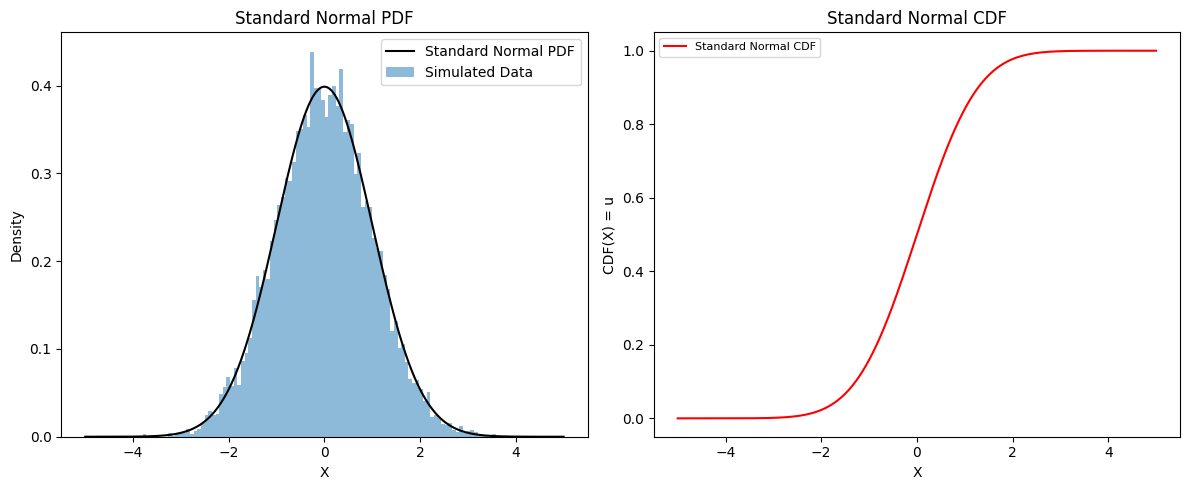
\includegraphics[width=1\linewidth]{3Theory/pictures/CDFandPDF1D.png}
    \caption{Illustration of a \gls{PDF} (left) and \gls{CDF} (right) for a random variable $X$, being standard normally distributed, in one dimension.}
    \label{fig:PDFandCDF1D}
\end{figure}
\todo{Make Left Right pictures}

When dealing with multiple assets the notion of a \gls{CDF} generalizes to a multivariate \gls{CDF}. To define a multivariate \gls{CDF} formally in two dimensions we will need to define the $H$-volume of a function in two dimensions and what the meaning of a function being 2-increasing is. This is done in the same manner as in \citet[p.~8]{Nelsen2006} in \Cref{def:H-volume} and \Cref{def:2-Increasing}.

\begin{definition}\label{def:H-volume} \textbf{H-Volume} \citet[p.~8]{Nelsen2006}\\
    Let $u$ and $v$ be nonempty subsets of $\bar{R} = [-\infty, \infty]$, and let $H$ be a two-place real function such that $\D H = u\times v$. Let $B = [u_1,u_2]\times[v_1,v_2]$  be a rectangle all of whose vertices are in $\D H$. Then
    the \emph{H-volume} of $B$ is given by
    \begin{align*}
        V_H(B) = H(u_2,v_2) - H(u_2,v_1) - H(u_1,v_2) + H(u_1,v_1).
    \end{align*}
\end{definition}

\begin{definition}\label{def:2-Increasing} \textbf{2-increasing} \citet[p.~8]{Nelsen2006}\\
     A 2-place real function $H$ is \emph{2-increasing} if its $H$-volume $V_H(B)\geq0$, for all rectangles B whose vertices lie in $\D H$.
\end{definition}

The notion of a 2-increasing function is illustrated in \Cref{fig:2-Increasing}. In the figure, the left picture shows a function that is 2-increasing meaning that it is increasing in both directions. The right picture illustrates when a function is not 2-increasing and how this will be captured by the $H$-volume of the function. This property is needed to define a \gls{CDF} in several dimensions, as done by \citet[p.~17]{Nelsen2006}, in \Cref{def:JointCDF}. 

\begin{figure}
    \centering
    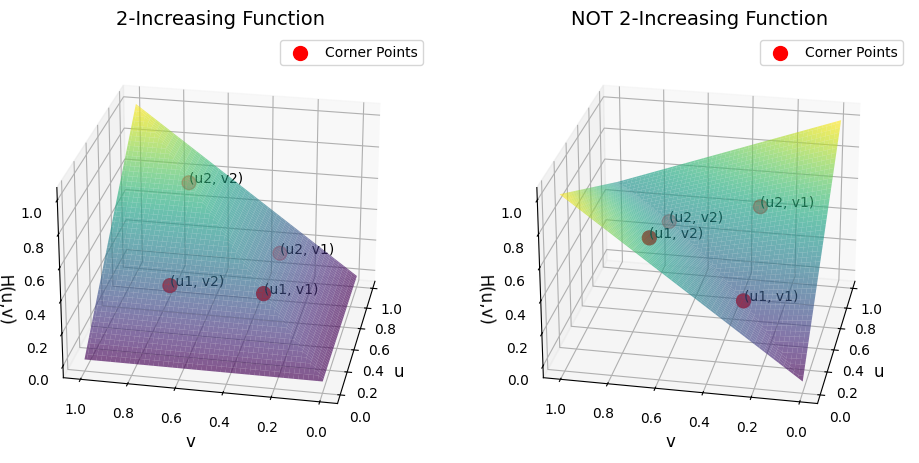
\includegraphics[width=1\linewidth]{3Theory/pictures/2increasingAndNot.png}
    \caption{Illustration of what it means for a function to be, and not to be, 2-increasing using the definition of the $H$-volume.}
    \label{fig:2-Increasing}
\end{figure}
\todo{Make Left Right pictures}



\begin{definition}\label{def:JointCDF} \textbf{Joint CDF} \\
    A \emph{joint distribution function} or joint \gls{CDF} is a function $F$ with domain $\bar{R}^2 = [-\infty, \infty]^2$ such that 
    \begin{compactenum}
        \item $F$ is 2-increasing; 
        \item $F(x_1,-\infty)= F(-\infty, x_2) = 0$, and $F(\infty,\infty)=1$.
    \end{compactenum}
\end{definition}

As in the univariate case the function value of the joint \gls{CDF} at any point in $\mathrm{Dom}X\times\mathrm{Dom}Y$ $\bar{R}^2$ is the probability of being below that point. In the two-dimensional setting, it is the probability of a point ending up below the point in both dimensions simultaneously. 

We can also define a \gls{PDF} in two dimensions as done by \citet[p.~235]{DevoreBerk2012} in \Cref{def:JointPDF}.

\begin{definition}\label{def:JointPDF} \textbf{Joint PDF} \\
    Let $X$ and $Y$ be continuous random variables. Then $f(x, y)$ is the \emph{joint} \gls{PDF} for $X$ and $Y$ if for any two-dimensional set $A$ 
    \begin{align*}
        P[(X,Y) \in A] =  \iint_A f(x,y)dxdy.
    \end{align*}
    
    In particular, if $A$ is the two-dimensional rectangle $\{(x,y) : a\leq x \leq b, c\leq y \ \leq d\}, $ then
    \begin{align*}
        P[(X,Y) \in A] = P(a\leq X \leq b, c \leq Y \leq d) =\int_a^b\!\!\!\int_c^d f(x,y)dxdy.
    \end{align*}
\end{definition}

\begin{remark}
    As seen in the univariate case, the same applies to the bivariate case. To be a candidate to be a joint \gls{PDF} $f(x,y)$ must satisfy 
    \begin{align*}
        &f(x,y) \geq 0, \;\mathrm{and} \\
        &\int_{-\infty}^{\infty}\!\int_{-\infty}^{\infty}f(x,y)dxdy=1.
    \end{align*}    
\end{remark}


Analogously to the univariate setting, the joint \gls{PDF} and \gls{CDF} are illustrated to give a visual understanding. In \Cref{fig:JointCDFandPDF} the left picture shows a joint \gls{PDF} for the random variable $X = (X_1, X_2)$, being standard normally distributed with zero correlation. In the right picture, the joint \gls{CDF} is displayed. 

\begin{figure}
    \centering
    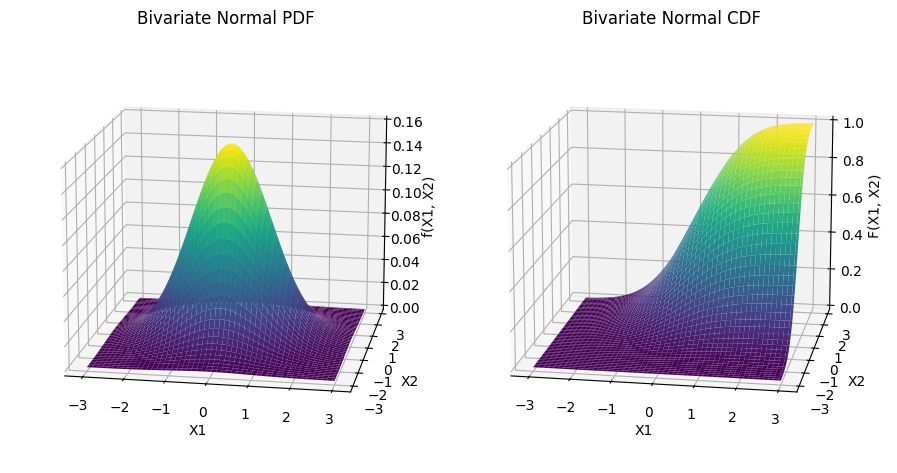
\includegraphics[width=1\linewidth]{3Theory/pictures/MultivariatePDFandCDF.png}
    \caption{Illustration of a \gls{PDF} (left) and \gls{CDF} (right) for a two dimensional random variable $X = (X_1,X_2)$, being standard normally distributed.}
    \label{fig:JointCDFandPDF}
\end{figure}
\todo{Make Left Right pictures}

The \gls{PIT} refers to transforming a continuous random variable to a uniformly distributed random variable. 
This maps the domain of a continuous one-dimensional random variable through its \gls{CDF} to the $[0,1]$ space, which may in the sequel be referred to as \emph{probability space}. This transformation will be central when defining copulas and is introduced in \Cref{the:PIT} as done in \citet[p.~27]{Danielsson2011}. 

\begin{theorem}\label{the:PIT} \textbf{Probability integral transform} \\
    Let $X$ be a continuous random variable with distribution function $F$. Define a new random variable $U = F(X)$, then $U \sim \mathrm{unif}(0,1)$. 
\end{theorem}

The probability integral transform is illustrated in \Cref{fig:PIT}. We can think of the \gls{PIT} as a method of mapping all observed data points on $\D X$  to probability space. In the figure, this can be seen as the dotted lines representing data points being mapped. 

Deeply connected to the \gls{PIT} is the \gls{ITM}, which is a method of generating random numbers from a given distribution. The method is based on the \gls{PIT} and works as defined by \Citet[p.~54]{glasserman2004monte}.
\begin{definition}\label{def:InverseTransformMethod}
    \textbf{Inverse transform method} \\
    The \emph{inverse transform method} is a method of generating random numbers from a given distribution.
    \begin{compactenum}
        \item Generate random numbers $U \sim \mathrm{Unif}(0,1)$;
        \item Insert the random numbers in the inverse \gls{CDF} of the desired distribution such that $X = F^{-1}(U)$.
    \end{compactenum}
    The random variable $X$ will then be distributed according to the desired distribution. That is $P(X\leq x) = F(x)$ for all $x$.
\end{definition}

The inverse transform method is illustrated in \Cref{fig:ITM} and can be seen as performing the \gls{PIT} in reverse. In the figure the red line is the inverse \gls{CDF} from which the sample is desired to be. The dotted lines represent the random numbers generated from the uniform distribution. The random numbers are then inserted into the inverse \gls{CDF} to obtain the desired sample.

\begin{figure}[h]
    \centering
    \begin{subfigure}[t]{0.45\linewidth}
        \centering
        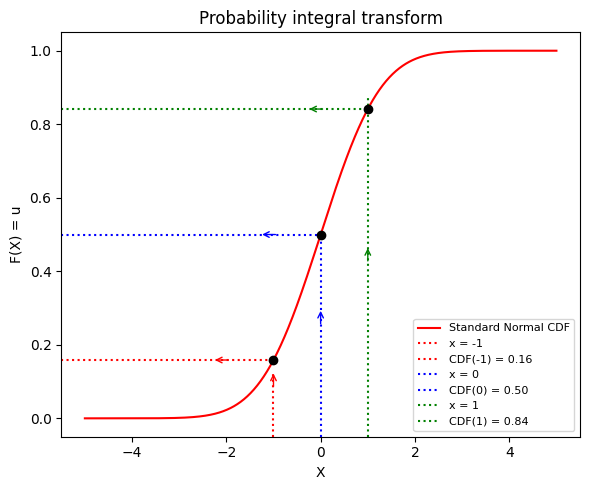
\includegraphics[width=\linewidth]{3Theory/pictures/ProbabilityIntegralTransform.png}
        \caption{Illustration of how the probability integral transform is used to transform realizations of a random variable $X$ having distribution function $F$ into a uniformly distributed random variable $U = F(X)$.}
        \label{fig:PIT}
    \end{subfigure}
    \hfill
    \begin{subfigure}[t]{0.45\linewidth}
        \centering
        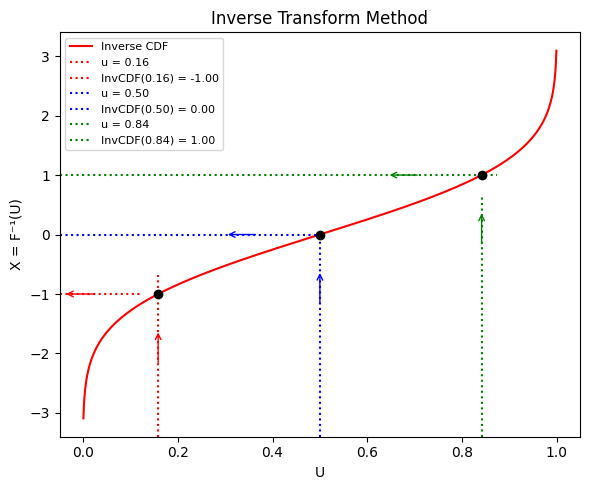
\includegraphics[width=\linewidth]{3Theory/pictures/InverseTransformMethod.png}
        \caption{Illustration of the inverse transform method and how it is used to generate random numbers from a given distribution given sampled points from a uniform distribution.}
        \label{fig:ITM}
    \end{subfigure}
    \caption{Probability Integral Transform and Inverse Transform Method.}
    \label{fig:TransformMethods}
\end{figure}


% \begin{figure}
%     \centering
%     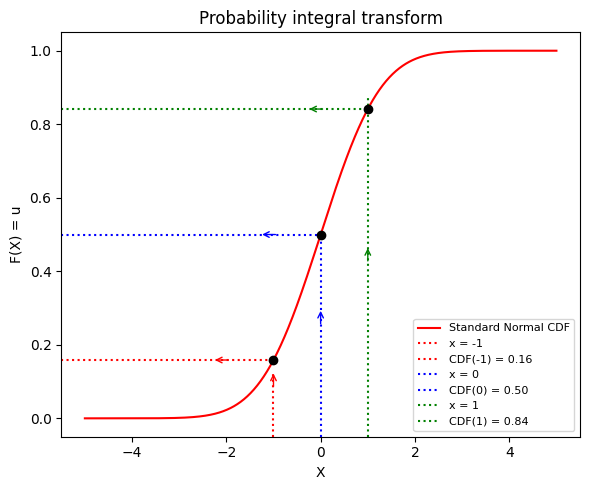
\includegraphics[width=0.45\linewidth]{3Theory/pictures/ProbabilityIntegralTransform.png}
%     \caption{Illustration of how the probability integral transform is used to transform realizations of a random variable $X$ having distribution function $F$ into a uniformly distributed random variable $U = F(X)$. }
%     \label{fig:PIT}
% \end{figure}
% \begin{figure}
%     \centering
%     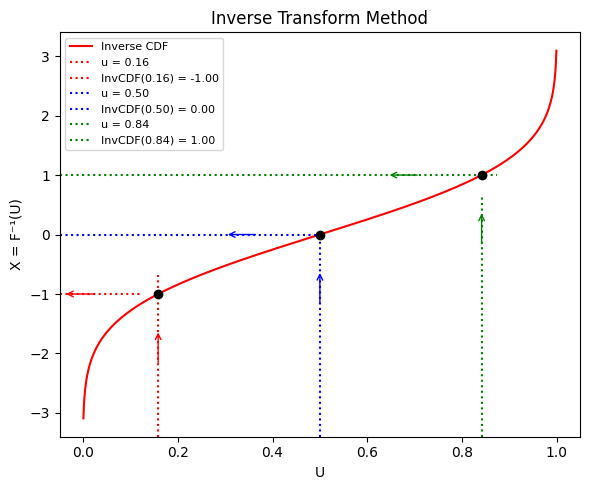
\includegraphics[width=0.45\linewidth]{3Theory/pictures/InverseTransformMethod.png}
%     \caption{Illustration of the inverse transform method and how it is used to generate random numbers from a given distribution given sampled points from a uniform distribution.}
%     \label{fig:ITM}
% \end{figure}


Another important notion is that of a marginal distribution of a joint distribution, which can be thought of as the distribution if only considering one of the dimensions that the joint distribution is made up of. The marginal \gls{CDF} and \gls{PDF} are defined in \Cref{def:MarginalCDF} and \Cref{def:MarginalPDF} respectively, in the same way as in \citet[p.~81]{evans2004probability} and \citet[p.~34]{wasserman2010statistics} respectively. 

\begin{definition}\label{def:MarginalCDF}
    \textbf{Marginal \gls{CDF}} 
    Let $X$and $Y$ be two random variables having joint \gls{CDF} $F_{X,Y}$, then the \gls{CDF} $F_X$ of $X$ can be obtained from $F_{X,Y}$ because
    \begin{align*}
        F_X(x) =P(X\leq x)
        =P(X\leq x,Y \leq \infty)
        =\lim_{y\to\infty} F_{X,Y}(x,y).
    \end{align*}
    $F_X$ is called the \emph{marginal distribution function} or marginal \gls{CDF} of $X$. The marginal distribution $F_Y$ can be obtained similarly. 
\end{definition}

\begin{definition}\label{def:MarginalPDF}
    \textbf{Marginal \gls{PDF}}
    For a continuous random variable, with domain $\mathrm{Dom}X\times \mathrm{Dom}Y$ $f_{X,Y}$, having joint \gls{PDF} $f_{X,Y}$, the \emph{marginal density function} or marginal \gls{PDF} of $X$ is given by
    \begin{align*}
        f_X(x) = \int_{-\infty}^\infty f_{X,Y}(x,y)dy.
    \end{align*}
    The marginal density $f_Y$ can be obtained similarly. 
\end{definition}

In \Cref{fig:MarginalCDF} the notion of a marginal distribution is visualized. In the left figure, a joint \gls{CDF} is shown to connect to the prior explanation of a \gls{CDF}. If the distribution is rotated to show it straight from one direction, as shown in the right figure, we can see the marginal distribution. In this case, it is the marginal distribution of $X_2$ that is displayed in red. This figure is of course simplified as it would not be plausible to view the limit when $X_1 \to \infty$.

\begin{figure}
    \centering
    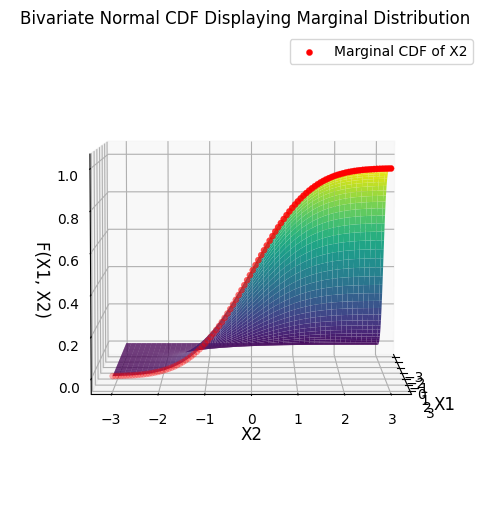
\includegraphics[width=1\linewidth]{3Theory/pictures/MarginalIllustrated.png}
    \caption{Illustration of what the marginal \gls{CDF} looks like for a bivariate normal distribution.   }
    \label{fig:MarginalCDF}
\end{figure}
\todo{Make Left Right pictures}


To conclude this subsection, we will show how the \gls{PIT} is utilized to transform data to the probability space and explain how it sets the stage for copulas. \Cref{fig:PITonData} illustrates how the \gls{PIT} is used to transform two-dimensional data into the two-dimensional probability space, by transforming through each of the marginal distributions separately. This is done for standard normally distributed data with and without correlation in (b) and (a) respectively, to highlight the differences in the distribution of points in the probability space when dependence is present and not in (d) and (c) respectively.

\begin{figure}
    \label{fig:PITonData}
    \centering
    \begin{minipage}{0.4\textwidth}
        \centering
        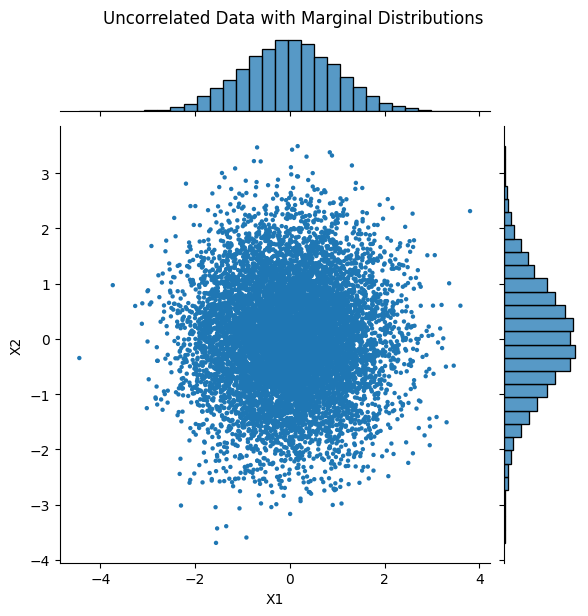
\includegraphics[width=\textwidth]{3Theory/pictures/UncorrelatedScatter.png}
        \subcaption{ Uncorrelated data from a bivariate standard normal distribution.}
    \end{minipage}
    \hfill
    \begin{minipage}{0.4\textwidth}
        \centering
        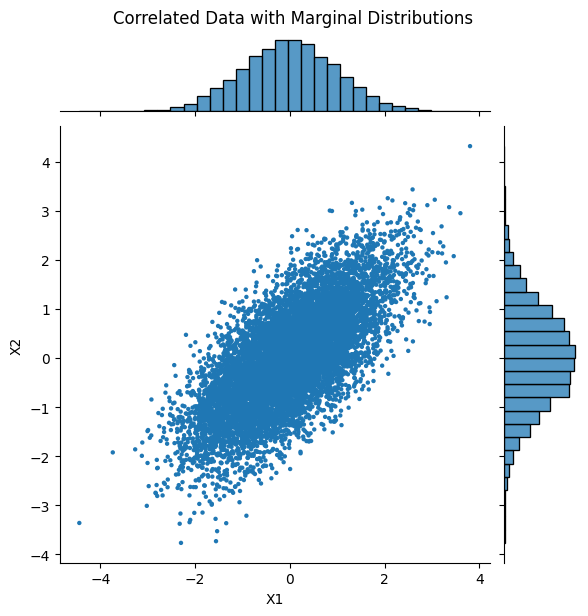
\includegraphics[width=\textwidth]{3Theory/pictures/CorrelatedScatter.png}
        \subcaption{Correlated data from a bivariate standard normal distribution.}
    \end{minipage}
    \vfill
    \begin{minipage}{0.4\textwidth}
        \centering
        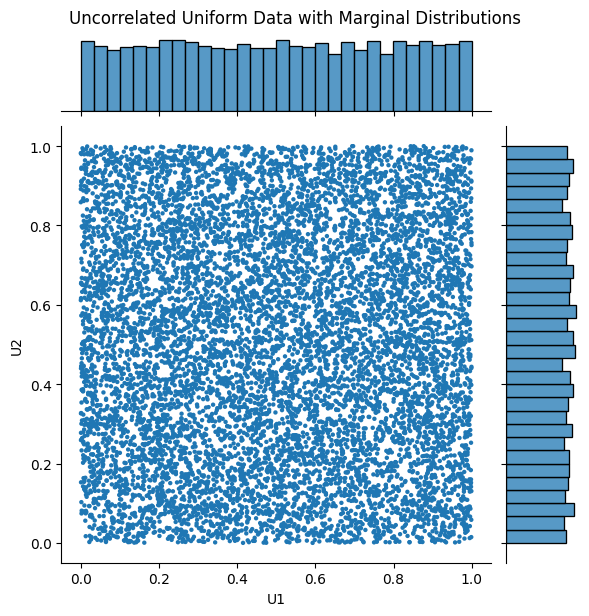
\includegraphics[width=\textwidth]{3Theory/pictures/UncorrelatedUniformScatter.png}
        \subcaption{Data in the probability space after applying the \gls{PIT} to uncorrelated normally distributed data.}
    \end{minipage}
    \hfill
    \begin{minipage}{0.4\textwidth}
        \centering
        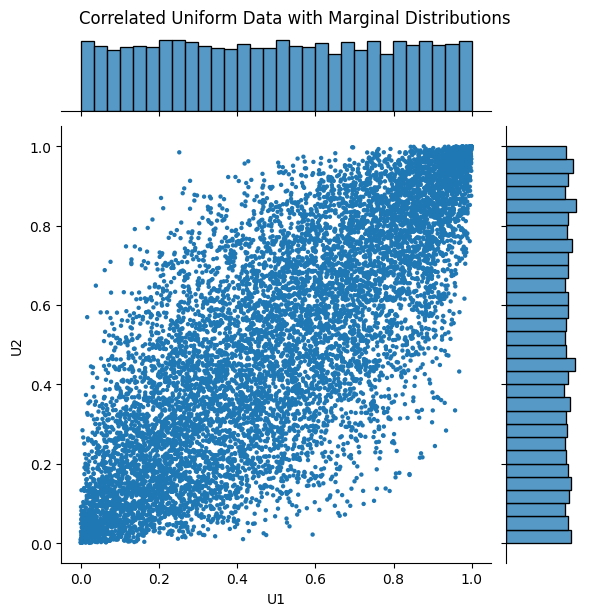
\includegraphics[width=\textwidth]{3Theory/pictures/CorrelatedUnoformScatter.png}
        \subcaption{Data in the probability space after applying the \gls{PIT} to correlated normally distributed data.}
    \end{minipage}
    \caption{Illustration of how the \gls{PIT} is used to transform two-dimensional data into the $[0,1]$-domain by considering the marginal distribution of each dimension separately.}
\end{figure}

Before introducing copulas in the next section we can simply describe the setting for copulas as \gls{CDF} of the data after having transformed it into the probability space using the \gls{PIT}. Relating to \Cref{fig:PITonData} we the copula is the \gls{CDF} of the data in (c) or (d).


\textbf{Maximum likelihood}
Another important concept which will be used when fitting the different copulas is the \gls{MLE}. To illustrate what it is, we first need to define the likelihood function as done by \Citet[p.~122]{wasserman2010statistics}
\begin{definition}
    \textbf{Likelihood function}
    The likelihood function for a sample of observations $X_1,\dots,X_n$ being $\mathrm{IID}$ with \gls{PDF} $f(x;\theta)$ is defined by 
    \begin{align*}
        \mathcal{L}_n(\theta) = \prod_{i=1}^n f(X_i;\theta).
    \end{align*}
\end{definition}

Usually, the likelihood function becomes very small when the sample size increases. This is because the likelihood is often a value smaller than one, and a product of such values often goes to zero. Therefore, it is common to instead of using the likelihood function use the log likelihood function defined by 
\begin{align*}
    l_n(\theta) = \log(\mathcal{L}_n(\theta)).
\end{align*}
We can see that the logarithm makes the product sum into a regular sum such that 
\begin{align*}
    l_n(\theta) = \log \left( \prod_{i=1}^n f(X_i;\theta) \right)= \sum_{i = 1}^n \log( f(X_i;\theta)).
\end{align*}

We can now define the \gls{MLE} as done by \Citet[p.~122]{wasserman2010statistics}
\begin{definition}
    The \emph{maximum likelihood estimator}, denoted by $\hat\theta_n$, is the value of $\theta$ that maximizes $\mathcal{L}_n(\theta)$.
\end{definition}
Maximizing the likelihood function is equivalent to maximizing the log likelihood function, meaning that the parameter estimate is the same \Citet[p.~123]{wasserman2010statistics}. 


%%%%%%%%%%%%%%%%%%%%%%%%%%%%%%%%%%%%%%%%%%%%%%%%%%%%%%%%%%%%%%%%%%%%%%%%%%%%%%
%%%% Copula theory
%%%%%%%%%%%%%%%%%%%%%%%%%%%%%%%%%%%%%%%%%%%%%%%%%%%%%%%%%%%%%%%%%%%%%%%%%%%%%%
\subsection{Copula Theory}\label{sec:CopulaTheory}
Now that we have a fundamental understanding of some probability theory we can introduce copulas. To do so we will need to define what it means for a function to be grounded, in \Cref{def:grounded}, and what it means to have margins, in \Cref{def:margins}, \citet[p.~9]{Nelsen2006}.

\begin{definition}\label{def:grounded}\textbf{Grounded} \\
    Consider a function on the domain $S_1\times S_2$ where $S_1$ and $S_2$ have the smallest elements $a_1$ and $a_2$ respectively. A function $H$ from $S_1\times S_2$ into $\mathbf{R}$ is \emph{grounded} if $H(x,a_2)= H(a_1,y) = 0 \;\mathrm{for \;all\;} (x,y) \in S_1\times S_2.$
\end{definition}

\begin{definition}\label{def:margins}
    \textbf{Margins}\\
    Consider a function on the domain $S_1\times S_2$ where $S_1$ and $S_2$ have the largest elements $b_1$ and $b_2$ respectively. A function $H$ from $S_1\times S_2$ into $\mathbf{R}$ has \emph{margins} $F$ and $G$ given by
    \begin{align*}
        \mathrm{Dom}F = S_1, \;\mathrm{and }\; F(x) = H(x,b_2) \;\mathrm{for \;all\;} x \in S_1\\
        \mathrm{Dom}G = S_2, \;\mathrm{and }\; G(x) = H(b_1,y) \;\mathrm{for \;all\;} y \in S_2.
    \end{align*}
\end{definition}

\Cref{fig:GroundedAndMargins} illustrates what \Cref{def:grounded} and \Cref{def:margins} means when $S_1$ and $S_2$ are both the probability space. The blue points show what it means to be grounded and the red points show what it means to have margins. 

%\todo{change the axes}
\begin{figure}
    \centering
    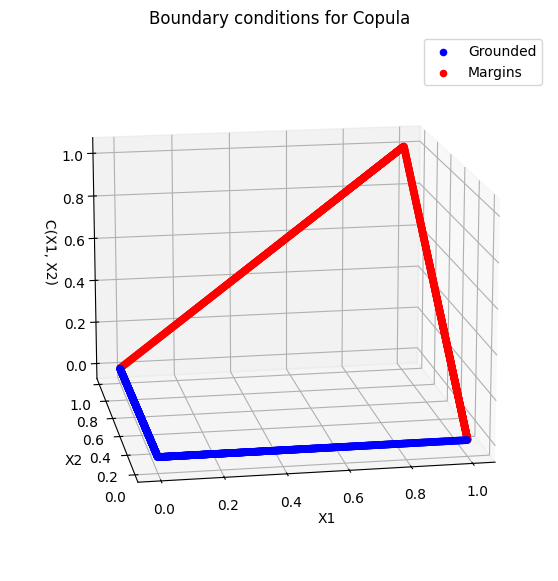
\includegraphics[width=0.5\linewidth]{3Theory/pictures/MarginsAndGrounded.png}
    \caption{Illustration showing what it means for a function to be grounded and to have margins.}
    \label{fig:GroundedAndMargins}
\end{figure}

Now we can formally define what a copula is. This is done as in \citet[p.~10]{Nelsen2006} in \Cref{def:copula}.
\begin{definition}\label{def:copula}
            \textbf{Copula in 2 dimensions}\\
            Equivalently, a copula is a function $C$ from $\mathrm{I}^2=[0,1]^2$ to $\mathrm{I} = [0,1]$ with the following properties:
            \begin{enumerate}
                \item For every $u, v \in \mathrm{I}$,
                \begin{align*}
                    C(u,0) &= C(0,v) = 0,\\
                    C(u,1) &= u, \; \mathrm{and } \; C(1,v) = v;
                \end{align*}
                \item For every $u_1, u_2, v_1, v_2 \in \mathrm{I}$ such that $u_1 \leq u_2$ and $v_1 \leq v_2$,
                \begin{align*}
                    C(u_2,v_2) - C(u_2,v_1) - C(u_1,v_2) + C(u_1,v_1) \geq 0.
                \end{align*}
            \end{enumerate}
\end{definition}

So, to describe what a copula is in simpler terms, it is a \gls{CDF} capturing the dependence between points on the probability space, obtained by performing the \gls{PIT} on each marginal distribution. 

A fundamental theorem connected to copulas is described in \Cref{the:Sklars}, as formulated by \citet[p.~18]{Nelsen2006}. 
\begin{theorem}\label{the:Sklars}
        \textbf{Theorem: Sklar's theorem} \\
        Let $H$ be a joint distribution function with margins $F$ and $G$ then there exists a copula $C$ such that for all $x,y \in \bar{\mathbf{R}} = \left[-\infty, \infty \right]$, 
        \begin{align}
            H(x,y) = C(F(x), G(y)). \label{eq:Sklar}
        \end{align}
        If $F$ and $G$ are continuous, then $C$ is unique; otherwise, $C$ is uniquely determined on $\mathrm{Ran}(F)\times\mathrm{Ran}(G)$. Conversely, if $C$ is a copula and $F$ and $G$ are distribution functions, then the function $H$ is a joint distribution function with margins $F$ and $G$.
\end{theorem}

\Cref{fig:CDFtoCopula} illustrates the correspondence, given in \Cref{eq:Sklar}, between a bivariate normal \gls{CDF} and its corresponding copula function. The copula has the same function value as the \gls{CDF} in each point where the mapping of points in $X_1\times X_2$ to $[0,1]\times[0,1]$ is done by the \gls{PIT}. The left picture shows the joint \gls{CDF} on the $\bar{R}^2$ domain. The right picture shows the corresponding copula function which lives in probability space. Hence, the difference between the joint \gls{CDF} and the copula is that the copula only exists on the unit square. 

\begin{figure}
    \centering
    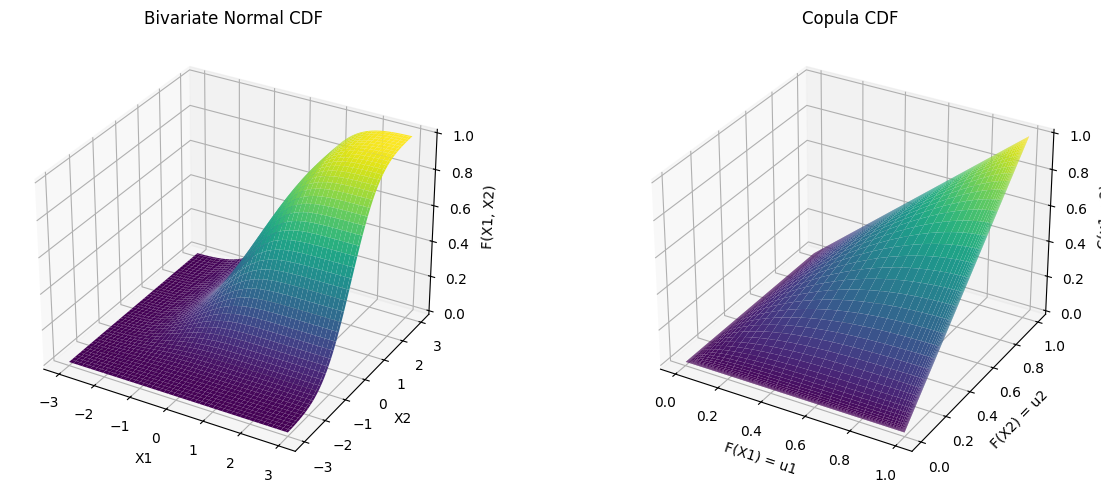
\includegraphics[width=1\linewidth]{3Theory/pictures/Copula.png}
    \caption{Illustration showing the correspondence between a bivariate normal \gls{CDF} and its corresponding copula function.}
    \label{fig:CDFtoCopula}
\end{figure}
\todo{fix Picture so that it isn't cut}

Sometimes it can be more convenient to write the \Cref{eq:Sklar} theorem in terms of the marginal probabilities $u_i$ rather than the marginal distributions $x_i$. It can be done by utilizing that $F_i(x_i) = u_i$ and $F_i^{-1}(u_i)= x_i$ so that 
\begin{align*}
    H(F_1^{-1}(u_1),F_2^{-1}(u_2))=H(x_1,x_2) = C(F_1(x_1), F_2(x_2))= C(u_1, u_2).
\end{align*}

Another important result for copulas is that they are translation invariant, the meaning of this is presented in \Cref{the:TranslationInvariance}, as done by \citet[p.~25]{Nelsen2006}.

\begin{theorem}\label{the:TranslationInvariance}
        \textbf{Theorem: Translation Invariance}\\
        Let $X$ and $Y$ be continuous random variables with copula $C_{X, Y}$. If $\alpha$ and $\beta$ are strictly increasing on $Ran(X)$ and $Ran(Y)$, respectively, then $C_{\alpha(X),\beta(Y)}  = C_{X,Y}$. Thus $C_{X, Y}$ is invariant under strictly increasing transformations of $X$ and $Y$.
\end{theorem}

From the requirements for a function to be a copula given in the definition of a copula in \Cref{def:copula} one can obtain bounds for how a copula can look. These bounds are defined as in \Cref{thm:FrechetBounds}.
    
\begin{theorem}\label{thm:FrechetBounds}
    \textbf{Fréchet-Hoeffding bounds} (\Citet[p.~7]{Schmidt2006} or \Citet[p.~11]{Nelsen2006})
    Consider a copula $C(\mathbf{u}) = C(u_1,u_2)$. Then the $C$ is bounded by
    \begin{align*}
        L(u_1,u_2) &\leq C(u_1,u_2) \leq U(u_1,u_2),\; \mathrm{ where}\\
        L(u_1,u_2) &= (u_1+u_2-1)^+\\
        U(u_1,u_2) &= \mathrm{min}(u_1,u_2).
    \end{align*}
    $L$ and $U$ are referred to as the Fréchet-Hoeffding lower and upper bounds respectively. 
\end{theorem}

Another important copula is the \emph{independence copula} or product copula corresponding to when the two marginal distributions are independent. The independence copula is defined by (\citet[p.~712]{BrigoMercurio2006} or \citet[p.~7]{Schmidt2006}) as
\begin{align*}
    \Pi(u_1,u_2) = u_1u_2.
\end{align*}

\Cref{fig:FrechetBounds} illustrates the upper (left) and lower (middle) bounds for copulas. We can think of it as if these bounds define a space where all copulas must be confined. One such copula is the independence copula (right) corresponding to the case when random variables are independent. 

\begin{figure}
    \centering
    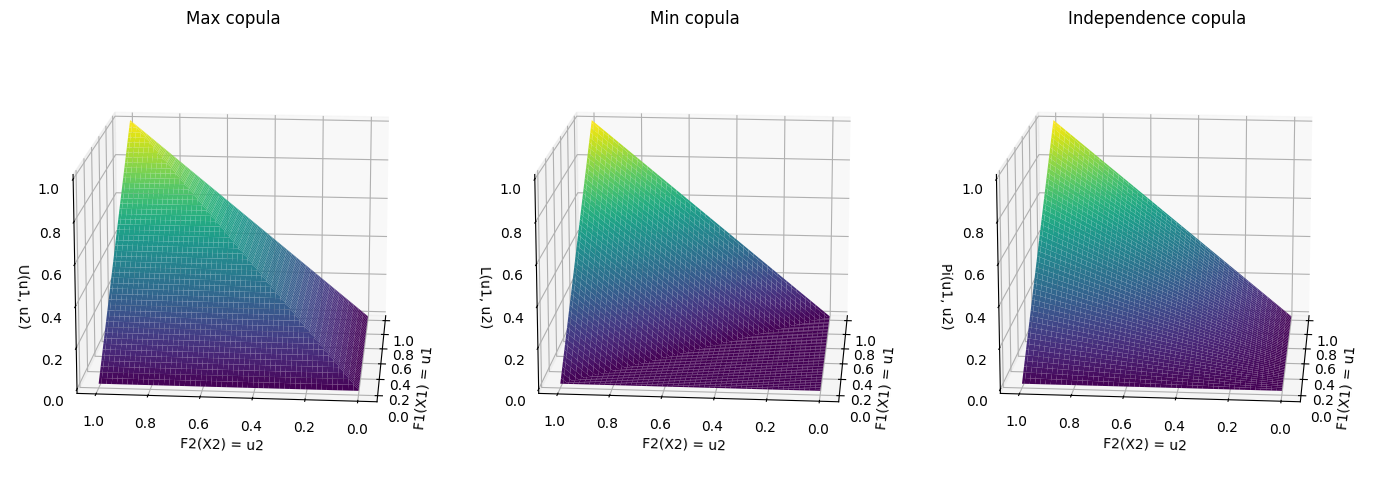
\includegraphics[width=1.\linewidth]{3Theory/pictures/FrechetBounds.png}
    \caption{Illustration of the Fréchet-Hoeffding upper $U$ (left), and lower $L$ (middle) bounds, as well as the independence copula $\Pi$ (right).}
    \label{fig:FrechetBounds}
\end{figure}

We have now discussed what copula functions are and arrived at that copulas are \gls{CDF}s on the unit square. When fitting copulas to data using \gls{MLE} it is often useful to have the copula \gls{PDF}. Deriving the copula \gls{PDF} is not as straightforward as one might initially think. Therefore we will derive the copula \gls{PDF} in the general case. Let $C(u_1,u_2)$ be the cpula \gls{CDF} you want to derive the \gls{PDF} for. The copula \gls{PDF} is defined as the second derivative of the copula \gls{CDF} with respect to $u_1$ and $u_2$.
\begin{align*}
    c(u_1,u_2) = \frac{\partial^2C(u_1,u_2)}{\partial u_1\partial u_2} = 
    \frac{\partial^2F(F_1^{-1}(u_1),F_2^{-1}(u_2))}{\partial u_1\partial u_2}
    = \\ f(F_1^{-1}(u_1),F_2^{-1}(u_2)) \frac{d}{du_1} F_1^{-1}(u_1)  \frac{d}{du_2} F_2^{-1}(u_2),
\end{align*}
where it can be shown that 
\begin{align*}
    \frac{d}{du_i} F_i^{-1}(u_i) = \frac{1}{f_i(F_i^{-1}(u_i))}.
\end{align*}
In the above equations, $F_i$ is the i:th marginal distribution function, \gls{CDF}, and $f_i$ is the marginal density function \gls{PDF}, $F$ is the joint distribution function.   

Hence the copula \gls{PDF} can be written as 
\begin{align*}
    c(u_1,u_2) &= f(F_1^{-1}(u_1),F_2^{-1}(u_2)) \frac{1}{f_1(F_1^{-1}(u_1))}\frac{1}{f_2(F_2^{-1}(u_2))}. 
\end{align*}

It can also be useful to write the copula in terms of data points that in the return space as this is typically where the data is observed
\begin{align*}
    c(u_1,u_2) &= f(F_1^{-1}(u_1),F_2^{-1}(u_2)) \frac{1}{f_1(F_1^{-1}(u_1))}\frac{1}{f_2(F_2^{-1}(u_2))},
\end{align*}
where $x_i = F_i^{-1}(u_i)$ and $f_i$ is the marginal \gls{PDF} of the i:th marginal distribution. 



%%%%%%%%%%%%%%%%%%%%%%%%%%%%%%%%%%%%%%%%%%%%%%%%%%%%%%%%%%%%%%%%%%%%%%%%%%%%
%%%% The need for copulas
%%%%%%%%%%%%%%%%%%%%%%%%%%%%%%%%%%%%%%%%%%%%%%%%%%%%%%%%%%%%%%%%%%%%%%%%%%%%
\subsubsection{Usefulness of copulas}

The following examples are to illustrate how correlation can fail to capture the true dependence between random variables. The first example shows how correlation fails to capture the dependence between two random variables that are dependent but uncorrelated and is inspired by \Citet[p.~21]{Danielsson2011}. The second example shows how correlation underestimates the true dependence between two random variables that are dependent but not both normally distributed. This is to illustrate how correlation falls short as a measure of dependence, and that copulas can be a better alternative when estimating dependence between random variables. \Cref{ex:CorrelationUnderestimates} is provided with full derivations in the appendix, \Cref{sec:CorrelationUnderestimates}.

\begin{example}\label{ex:CorrelationFail}
    \textbf{Dependence is not always captured by correlation}\\
    Let $X$ be a random variable such that, $X \sim N(0,1)$. Obviously, $X$ and $X^2$ are dependent. The covariance, $\mathrm{Cov}(X,X^2)$ is 
    \begin{align*}
        \mathrm{Cov}(X,X^2) &= E \left[  (X-E\left[  X \right])(X^2-E\left[  X^2 \right])  \right]\\
         &=  E \left[  (X)(X^2-1)  \right]\\
         &= E \left[  X^3  \right] - E \left[  X  \right]\\
         &= 0-0 = 0 .
    \end{align*}
    Since $\mathrm{Cov}(X,X^2) = \rho_{X,X^2}\sigma_{X}\sigma_{X^2} = \rho_{X,X^2}$ this shows that $\rho_{X,X^2} = 0.$
    Hence, $X$ and $X^2$ are dependent but uncorrelated. This shows how correlation falls short as a method of capturing non-linear dependence.
    %\todo{Maybe illustrate how this problem is solved using a copula(example of how in Brigo)}
    
    % Using a copula instead we get
    % \begin{align*}
    % F_{X^2}(X^2) &= P(X^2 \leq x^2)\\
    % &= P(\sqrt{X^2} \leq \sqrt{x^2})\\
    % &= P(|X| \leq |x| )\\    
    % &=P(X\leq x) = U2 \neq U1.\\
    % \end{align*}

    % Since the absolute value signs information is lost and hence 
    % \begin{align*}
    %     P(U_1\leq u1, U_2\leq u2) = P(U_1\leq u1, U_1\leq u2) = \min(u_1,u_2).
    % \end{align*}
    
\end{example}

\begin{example}\label{ex:CorrelationUnderestimates}
    \textbf{Correlation underestimates the true dependence} \\
    Let $X$ be a random variable such that, $X \sim N(0,1)$. Obviously, $X$ and $e^X$ are dependent. The covariance, $\mathrm{Cov}(X,e^X)$ is
    \begin{align*}
        \mathrm{Cov}(X,e^X) &= E \left[  (X-E\left[  X \right])(e^X-E\left[  e^X \right])  \right]\\
        %  &=  E \left[  X(e^X-E\left[  e^X \right]) \right]\\
        %  &= E \left[  Xe^X  \right] - E \left[  X E \left[  e^X \right] \right]\\
        %  &= E \left[  Xe^X  \right]\\
        %  &= \int_{-\infty}^\infty xe^x \frac{1}{\sqrt{2\pi}} e^{\frac{-x^2}{2}} dx\\ %by definition of expectation for Cont. rand. var. 
        %  &=  \int_{-\infty}^\infty \frac{1}{\sqrt{2\pi}} x  e^{x -\frac{x^2}{2}} dx \\
        %  &= \int_{-\infty}^\infty \frac{1}{\sqrt{2\pi}} x  e^{-\frac{1}{2}(x-1)^2+\frac{1}{2} } dx \\
        %  &= \frac{e^\frac{1}{2}}{\sqrt{2\pi}}\int_{-\infty}^\infty x  e^{-\frac{1}{2}(x-1)^2 } dx\\
        %  & \mathrm{Let\;} u = x-1 \; \mathrm{then\;} x = u+1\\
        %  &= \frac{e^\frac{1}{2}}{\sqrt{2\pi}}\int_{-\infty}^\infty (u+1)e^{\frac{-u^2}{2}} du\\
        %  &= \frac{e^\frac{1}{2}}{\sqrt{2\pi}} \left( \int_{-\infty}^\infty ue^{\frac{-u^2}{2}}du +\int_{-\infty}^\infty e^{\frac{-u^2}{2}} du  \right) \\
        %  &= \frac{e^\frac{1}{2}}{\sqrt{2\pi}}\sqrt{2\pi}   \\
         &= e^{\frac{1}{2}}.\\
    \end{align*}
    If dividing with the standard deviations of $X$ and $e^X$ we get the correlation. To do this we need to calculate the variances of $X$ and $e^X$. We know that $\mathrm{Var}(X) = 1$ but need to calculate the variance of $e^X$. The variance of $e^X$ is calculated as
    \begin{align*}
        \mathrm{Var}(e^X) &= E[e^{2X}] - E[e^X]^2\\
        &= e^2 - e.
    \end{align*}
    The correlation is then calculated as
    \begin{align*}
        \mathrm{corr}(X,e^X) &= \frac{\mathrm{cov}(x,e^X)}{\sqrt{\mathrm{var}(x)} \sqrt{\mathrm{var}(e^X)}}  \approx 0.76. 
       % & = \frac{e^{\frac{1}{2}}}{1\sqrt{e^2-e}}\\
       % &=\sqrt{\frac{1}{e-1}} \approx 0.76. 
    \end{align*}
    If instead using the copula to calculate the correlation we can see that the correlation is not capturing the true dependence between $X$ and $e^X$. To see this we can use the \gls{PIT} to transform $X$ and $e^X$ into uniform random variables. If we let $F_X(X)=U_1$ be the normal data transformed to uniform random variables and $F_{e^X}(e^X)=U_2$ be the log-normal data transformed to uniform random variables we can see that 
    \begin{align*}
        F_{e^X}(e^X) &= P(e^X \leq e^x)\\
        &= P(\ln(e^X) \leq \ln (e^x))\\
        &=P(X\leq x) = U2 = U1.
    \end{align*}
    Since $U_1 = U_2$ we have 
    \begin{align*}
        P(U_1\leq u1, U_2\leq u2) = P(U_1\leq u1, U_1\leq u2) = \min(u_1,u_2).
    \end{align*}
    This is the upper copula given by the upper Fréchet-Hoeffding bound, which is the copula corresponding to maximum dependence. Hence, correlation underestimates the true dependence between the random variables given that maximum dependence under the correlation framework is one. This underestimation of the correlation is because of the assumption of a normal or students $t$ distribution which is violated with the lognormal variable in the example. This shows how copulas can capture dependence when correlation fails. 

    In \Cref{fig:ExamplePlots} some illustrations of \Cref{ex:CorrelationUnderestimates} are shown. The the true copula \gls{CDF} is shown in \Cref{fig:TrueCopulaExponential} this can be compared to the estimated copula using correlation in \Cref{fig:CorrelationEstimationExponential}. %\Cref{fig:exponentialDependenceScatterProb} shows the scatter plot of the data in the probability space illustrating what maximum dependence looks like in probability space. 
    \Cref{fig:exponentialDependenceScatterRet} shows the scatter plot of the data in the return space. This illustrates why correlation is insufficient as a dependency measure when the underlying dependence is non-linear. 
    
    % \begin{generalinstructions}
    %     Would be nice to tie this to something in finance. Such as the relationship between stocks returns and derivative prices.

    %     This shows that estimating the correlation in a setting when the different marginals are not both normal can be misleading. This is a problem in finance where one often uses correlation to estimate the dependence between different assets. This is especially true when using correlation to estimate the dependence between stocks and derivatives.
    % \end{generalinstructions}
\end{example}
    

\begin{figure}
    \centering
    \begin{minipage}{0.45\textwidth}
        \centering
        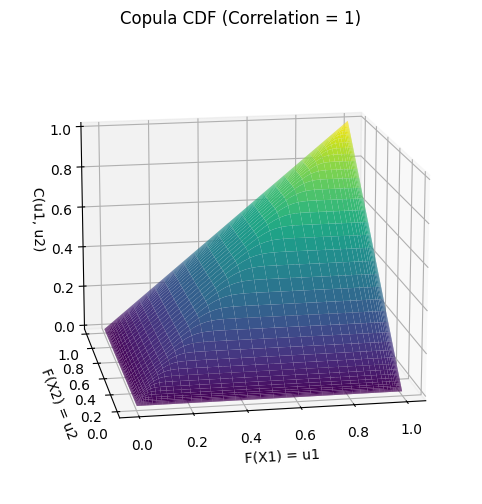
\includegraphics[width=\textwidth]{3Theory/pictures/TrueCopulaExponential.png}
        \subcaption{True copula \gls{CDF} for the example.}
        \label{fig:TrueCopulaExponential}
    \end{minipage}
    \hfill
    % \begin{minipage}{0.25\textwidth}
    %     \centering
    %     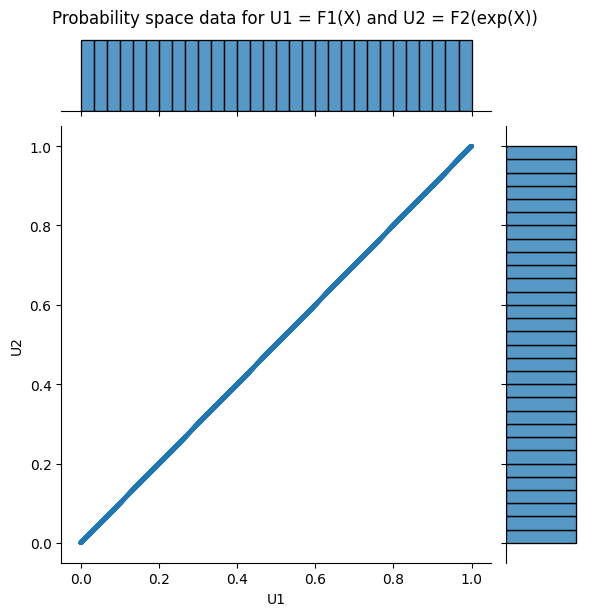
\includegraphics[width=\textwidth]{3Theory/pictures/exponentialDependenceScatterProb.png}
    %     \subcaption{Data in the probability space.}
    %     \label{fig:exponentialDependenceScatterProb}
    % \end{minipage}
    % \vfill
    \begin{minipage}{0.45\textwidth}
        \centering
        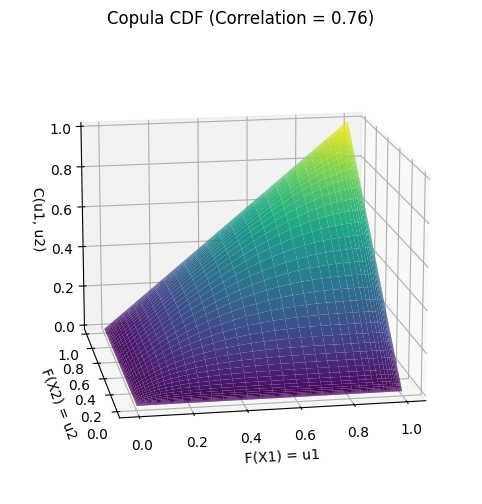
\includegraphics[width=\textwidth]{3Theory/pictures/CorrelationEstimationExponential.png}
        \subcaption{Estimated copula \gls{CDF} using correlation.}
        \label{fig:CorrelationEstimationExponential}
    \end{minipage}
    %\hfill
    \vfill
    \begin{minipage}{0.45\textwidth}
        \centering
        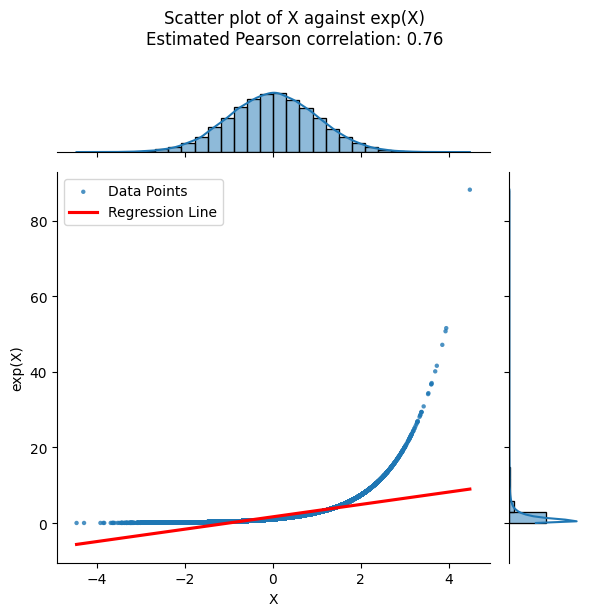
\includegraphics[width=\textwidth]{3Theory/pictures/exponentialDependenceScatterRet.png}
        \subcaption{Data in return space showing correlation estimate using the regression line.}
        \label{fig:exponentialDependenceScatterRet}
    \end{minipage}
    \caption{Figures illustrating how correlation breaks as a measure of dependence.}
    \label{fig:ExamplePlots}
\end{figure}

Up to now we have not yet provided an example of the usefulness of copulas. The next section will show an example of how copulas are useful in practice.

%%%%%%%%%%%%%%%%%%%%%%%%%%%%%%%%%%%%%%%%%%%%%%%%%%%%%%%%%%%%%%%%%%%%%%%%%%%%
%%%% Use for copula
%%%%%%%%%%%%%%%%%%%%%%%%%%%%%%%%%%%%%%%%%%%%%%%%%%%%%%%%%%%%%%%%%%%%%%%%%%%%
\subsubsection{Usecase for copula in practice}\label{sec:CopulaUseCase}
If there are several sources of randomness present in a system where monte carlo methods are used, potential dependence between the sources of randomness has to be taken into account. Copulas are a powerful tool for modeling the dependence structure between random variables. They allow for separation of the dependence and the marginal distributions. By using copulas, we can generate samples from multivariate distributions with specified marginals and a desired dependence structure by generating dependent marginally distributed uniform random numbers. These are then transformed to the desired marginal distributions using the inverse of the marginal \gls{CDF}s by the inverse transform method \Cref{def:InverseTransformMethod}.

Let $U = (U_1,U_2)$ be a point specified by two marginally uniformly distributed random variables $U_1$ and $U_2$ sampled from a copula giving them some dependence. Then random numbers $X = (X_1,X_2)$ with the dependence specified by the copula and desired marginal distributions can be generated by transforming the uniform random numbers using the \gls{ITM}. This is done by using the inverse of the marginal \gls{CDF}s as follows
\begin{align*}
    X_1 = F_1^{-1}(U_1); \\
    X_2 = F_2^{-1}(U_2).
\end{align*}

The usefulness of copulas in sampling is visualised in \Cref{fig:CopulaSampling}. The left figure shows a sample from a Clayton copula with $\alpha = 4$. The right figure shows the same sample after applying the \gls{ITM} using a standard normal distribution for each marginal. Note that the \gls{ITM} can be applied to each of the dimensions of the copula data thanks to the fact that copulas by definition have uniform marginals. 

\begin{figure}[h]
    \centering
    \begin{subfigure}[t]{0.45\linewidth}
        \centering
        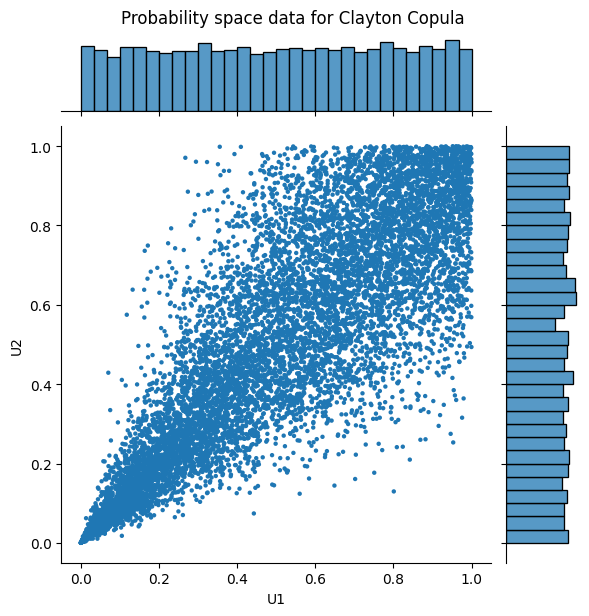
\includegraphics[width=\linewidth]{3Theory/pictures/ProbabilitySpaceClayton.png}
        \caption{Sample from a Clayton copula with $\alpha = 4$. } 
        \label{fig:ProbabilitySpaceDataClayton}
    \end{subfigure}
    \hfill
    \begin{subfigure}[t]{0.45\linewidth}
        \centering
        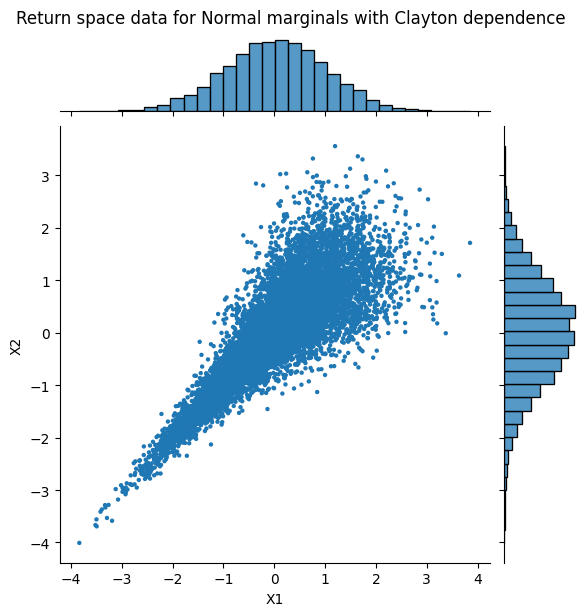
\includegraphics[width=\linewidth]{3Theory/pictures/ReturnSpaceDataClayton.png}
        \caption{Sample from Clayton copula after applying the inverse transform method using a standard normal distribution.}
        \label{fig:ReturnSpaceDataClayton}
    \end{subfigure}
    \caption{Illustration of sampling from a clayton copula with standard normal marginal distributions.}
    \label{fig:CopulaSampling}
\end{figure}


In the above example we have seen the usefulness of copulas in sampling. The example does not go into the nontrivial task of sampling from a copula. Therefore the next section introduces conditional sampling which is a method of sampling from a copula. 

\subsubsection{Conditional sampling from copulas}\label{sec:ConditionalSampling} from \Citet[p.~41]{Nelsen2006}\\
For some copulas samples can be generated using conditional sampling which works as follows. First, we generate two independent uniform random numbers $z_1,z_2 \sim \mathrm{Unif}(0,1)$. 
The first random number is calculated without respect for the second random number hence we set $u_2 =1$. We want to solve
\begin{align*}
    C(u_1,u_2) =z_1,
\end{align*}
for $u_1$ independently of $u_2$. 

By using that the copula is a \gls{CDF} and can be written as a probability we can see that 
\begin{align*}
    C(u_1,u_2) = P(U_1\leq u_1, U_2\leq u_2) = P(U_1\leq u_1,U_2 \leq 1) = P(U_1\leq u_1).
\end{align*} 
Since $u_2 = 1$ no constraint is enforced on $U_2$. By the definition of a copula we have that 
\begin{align*}
    C(u_1,1) = u_1 = z_1.
\end{align*}
So we set the first random number as $u_1 = z_1$.

The second random number is obtained by computing the conditional copula \gls{CDF} given the first random number. This is done by using the conditional copula \gls{CDF} defined as
\begin{align*}
    C_{2|1}(u_2|u_1) = \frac{\partial C(u_1,u_2)}{\partial u_1}.
\end{align*}
To compute the second random number we need to solve the equation
\begin{align*}
    C_{2|1}(u_2|u_1) = z_2,
\end{align*}
for $u_2$. That is
\begin{align*}
    u_2 = C^{-1}_{2|1}(z_2|z_1).
\end{align*}
The pair $(u_1,u_2)$ is now a sample from the copula. The method can be repeated to generate more samples from the copula. The requirement for the copula to be able to use this method is that the copula has a strictly increasing conditional copula. If not, the solution to the equation might not be unique which will cause problems in the solving step. 

\todo{$C^{-1}$ is the quasi inverse since copula can be flat} 

\subsubsection{Acceptance rejection sampling}\label{sec:AcceptanceRejection} 
Acceptance rejection sampling is a method of sampling from any distribution as long as the density function is known \Citet[p.~47]{RobertCasella2004}. The method works by generating a sample from a proposal distribution and then accepting or rejecting the sample based on a threshold. The sampling method is defined below as done by \Citet[p.~50]{RobertCasella2004}.

\begin{definition}
    \textbf{Acceptance rejection sampling}\\
    Let $X \sim f(x)$ and let $g(x)$ be a density function such that $M g(x) \geq f(x)$ for some constant $M \geq 1$. To sample $X \sim f$, we can generate   
    \begin{align*}
        Y \sim g \; \mathrm{and} \; U|Y = y \sim \mathrm{Unif}(0,Mg(y)),      
    \end{align*}
    until $0 \leq u \leq f(y)$.
\end{definition}
$M$ is a constant that scales $g$ so that it is always larger than $f$. In general, the standard uniform distribution can always be used as $g$ but it is often more efficient to use a distribution that is similar to the target distribution. If the proposal distribution is the uniform distribution $M$ is the maximum value of $f$.  

%%%%%%%%%%%%%%%%%%%%%%%%%%%%%%%%%%%%%%%%%%%%%%%%%%%%%%%%%%%%%%%%%%%%%%%%%%%%
%%%% Other Copulas
%%%%%%%%%%%%%%%%%%%%%%%%%%%%%%%%%%%%%%%%%%%%%%%%%%%%%%%%%%%%%%%%%%%%%%%%%%%%
\subsection{Other copulas}
This section introduces some of the most commonly used copulas. Some copulas are defined through known statistical distributions such as the Gaussian copula and the Student's t copula. Another type of copulas is the family of Archimedean copulas, of which the Clayton copula is an example.

%%%%%%%%%%%%%%%%%%%%%%%%%%%%%%%%%%%%%%%%%%%%%%%%%%%%%%%%%%%%%%%%%%%%%%%%%%%%
%%%% Gaussian Copula
%%%%%%%%%%%%%%%%%%%%%%%%%%%%%%%%%%%%%%%%%%%%%%%%%%%%%%%%%%%%%%%%%%%%%%%%%%%%
\subsubsection{Gaussian Copula}\label{sec:GaussianCopula}
A commonly used copula is the Gaussian copula which is derived from the centered multivariate normal distribution. 

Let $\boldsymbol{\Phi}_\Sigma(x_1,x_2)$ be the bivariate normal distribution \gls{CDF} with correlation matrix $\Sigma$. Let $\Phi(x)$ be the univariate normal \gls{CDF}. Then the Gaussian copula is defined, as in \citet[p.~112]{Umberto2004copulaMethods}  by 
\begin{align*}
    C_\Sigma(u_1,u_2) = \boldsymbol{\Phi}_\Sigma(\Phi^{-1}(u_1),\Phi^{-1}(u_2)).
\end{align*}

In the above expression $\Sigma$ is the correlation matrix in two dimensions 
\begin{align*}
    \Sigma = 
    \begin{bmatrix}
            1 & \rho_{1,2} \\
            \rho_{1,2} & 1
    \end{bmatrix},
\end{align*}
so in the sequel when $\rho$ is used it refers to $\rho_{1,2}$ in the correlation matrix.

The copula function, which is a \gls{CDF} can be expressed on integral form as done by \citet[p.~112]{Umberto2004copulaMethods}
\begin{align*}
     C_{\Sigma} (u_1,u_2)
    = \int_{-\infty}^{\Phi^{-1}(u_1)}\int_{-\infty}^{\Phi^{-1}(u_2)}
    \frac{1}{2\pi\sqrt{1-\rho^2}} \mathrm{exp}\left\{ - \frac{s^2-2\rho st+t^2}{2(1-\rho^2)}   \right\} dsdt.
\end{align*} 

The \gls{PDF} of the Gaussian copula function can be shown to be 
\begin{align*}
     c_{\Sigma} (u_1,u_2)
    = \frac{1}{\sqrt{1-\rho^2}} \mathrm{exp}\left\{  \frac{-2\rho^2\Phi^{-1}(u_1)^2  +2\rho \Phi^{-1}(u_1)\Phi^{-1}(u_2) -2\rho^2\Phi^{-1}(u_2)^2}{2(1-\rho^2)}   \right\},
\end{align*}
as stated in \citet[p.267]{Alexander2008}.



\textbf{Fitting}(alternative source: \Citet[pp.~281-283]{Alexander2008})
To fit the Gaussian copula to data we need to compute the correlation matrix $\Sigma$. This is done by first estimating the sample covariance matrix and then normalizing it to obtain the correlation matrix\footnote{See \url{https://support.sas.com/documentation/onlinedoc/ets/132/copula.pdf}. \textit{SAS/ETS\textsuperscript{\textregistered} 13.2 User's Guide}, p.523, SAS Institute Inc., Cary, NC, 2014. Last Accessed: 2025-04-24.}.%\Citet[p.~523]{SAS2014}. 

\textbf{Sampling}(alternative source: \Citet[p.~19]{Schmidt2006})
To sample from a Gaussian copula we can first generate a sample from the multivariate normal distribution with the desired correlation matrix $\Sigma$. This is done by multiplying a standard normal random vector with the Cholesky decomposition of the correlation matrix. The Cholesky decomposition can be thought of as a matrix square root of the correlation matrix. The resulting sample of correlated random numbers is then transformed to uniform random numbers using the \gls{PIT}. This is done by applying the univariate normal \gls{CDF} to each of the elements in the sample. The resulting sample is then a sample from the Gaussian copula\footnotemark[\value{footnote}]. %\footnote{\value{\footnote}} %\footnote{See \url{https://support.sas.com/documentation/onlinedoc/ets/132/copula.pdf}. \textit{SAS/ETS\textsuperscript{\textregistered} 13.2 User's Guide}, p.523, SAS Institute Inc., Cary, NC, 2014. Last Accessed: 2025-04-24.}.%\Citet[p.~523]{SAS2014}.



%%%%%%%%%%%%%%%%%%%%%%%%%%%%%%%%%%%%%%%%%%%%%%%%%%%%%%%%%%%%%%%%%%%%%%%%%%%%
%%%% Students Copula
%%%%%%%%%%%%%%%%%%%%%%%%%%%%%%%%%%%%%%%%%%%%%%%%%%%%%%%%%%%%%%%%%%%%%%%%%%%%
\subsubsection{Students t Copula}\label{sec:StudentsCopula} \citet[p.~116]{Umberto2004copulaMethods} 
The Student's $t$ copula can be defined similarly to the Gaussian copula above. We denote the Student's $t$ copula by 
\begin{align*}
    C_{\nu,\Sigma}(u_1,u_2) = \boldsymbol{t}(t_\nu^{-1}(u_1),t_\nu^{-1}(u_1)),
\end{align*}
as done by \citet[p.~268]{Alexander2008}, where $\nu >0$ is the degrees of freedom, $\boldsymbol{t}$ is the multivariate Student's $t$ distribution, $t$ is the univariate Student's $t$ distribution, and $\Sigma$ is the correlation matrix matrix.

The Student's $t$ copula \gls{CDF} is 
\begin{align*}
     C_{\nu,\Sigma}^t (u_1,u_2)
    = \int_{-\infty}^{t_\nu^{-1(u_1)}}\int_{-\infty}^{t_\nu^{-1(u_2)}}
    \frac{1}{2\pi\sqrt{1-\rho^2}} \left\{  1+ \frac{s^2-2\rho st+t^2}{\nu(1-\rho^2)}   \right\} dsdt,
\end{align*}
as defined by \citet[p.~116]{Umberto2004copulaMethods}. The corresponding copula \gls{CDF} is, by the same logic as for the Gaussian case, the integrand in the expression above times the two partial derivatives of the marginal distributions. The resulting expression for the copula \gls{PDF} $c_{\nu,\rho}$ is therefore 
\begin{align*}
    c_{\nu,\Sigma}(u_1,u_2) = \frac{\Gamma(\frac{\nu+2}{2})\Gamma(\frac{\nu}{2})\prod_{j=1}^2\left( 1+ \frac{t_\nu^{-1}(u_j)^2}{\nu}\right)^{\frac{\nu+2}{2}} } {\sqrt{\rho} \;\Gamma(\frac{\nu+1}{2})^{2}\left( 1+ \frac{t_\nu^{-1}(u_1)^2 + t_\nu^{-1}(u_2)^2 -2\rho t_\nu^{-1}(u_1) t_\nu^{-1}(u_2) }{\nu(1-\rho^2)}\right)},
\end{align*}
as stated by \Citet[p.~117]{Umberto2004copulaMethods}. In the above expression $\Gamma$ is the Euler gamma function.

\textbf{Fitting} 
To fit the Student's $t$ copula to data we need to compute the correlation matrix $\Sigma$ and the degrees of freedom $\nu$. It is common to first estimate the correlation matrix and then estimate the degrees of freedom using \gls{MLE} \Citet[p.~283]{Alexander2008}. In this thesis we will use the Pearson correlation to estimate the correlation matrix. 

\textbf{Sampling} (alternative source: \Citet[p.~19]{Schmidt2006})
Sampling from a Student's $t$ copula is similar to sampling from a Gaussian copula. First, we generate a sample from the multivariate Student's $t$ distribution with the desired correlation matrix $\Sigma$ and degrees of freedom $\nu$. This can be done by generating a sample $Z$ from a normal distribution with correlation matrix $\Sigma$ as described for the Gaussian copula. These normal random numbers can then be transformed into Student's $t$ distributed sample $X$ by the calculation $X = Z\sqrt{\frac{\nu}{s}} $, where s is a sample from a $\chi^2$ distribution with $\nu$ degrees of freedom. The resulting sample of correlated Student's $t$ random numbers is then transformed to uniform random numbers using the \gls{PIT}. This is done by applying the univariate Student's $t$ \gls{CDF} with $\nu$ degrees of freedom to each of the elements in the sample. The resulting sample is then a sample from the Student's $t$ copula\footnote{See \url{https://support.sas.com/documentation/onlinedoc/ets/132/copula.pdf}. \textit{SAS/ETS\textsuperscript{\textregistered} 13.2 User's Guide}, p.524, SAS Institute Inc., Cary, NC, 2014. Last Accessed: 2025-04-24.}.%\Citet[p.~524]{SAS2014}. 

%%%%%%%%%%%%%%%%%%%%%%%%%%%%%%%%%%%%%%%%%%%%%%%%%%%%%%%%%%%%%%%%%%%%%%%%%%%%
%%%% Clayton Copula
%%%%%%%%%%%%%%%%%%%%%%%%%%%%%%%%%%%%%%%%%%%%%%%%%%%%%%%%%%%%%%%%%%%%%%%%%%%%
\subsubsection{Clayton Copula}\label{sec:ClaytonCopula}
Archimedian copulas have the general expression  
\begin{align*}
    C(u_1,u_2) = \Psi^{-1}(\Psi(u_1),\Psi(u_2)),
\end{align*}
for some generator function $\Psi$, as defined by \Citet[p.~150]{Umberto2004copulaMethods}.

The Clayton copula, which is one instance of an Archimedean copula, uses the generator function
\begin{align*}
    \Psi(u) &=u^{-\alpha}-1, 
\end{align*}
and its inverse
\begin{align*}
    \Psi^{-1}(x) &= (x+1)^{\frac{-1}{\alpha}},
\end{align*}
where $\alpha > 0$. 

This gives the bivariate Clayton copula \gls{CDF}
\begin{align*}
    C(u_1,u_2) = (u_1^{-\alpha} + u_2^{-\alpha}-1)^{\frac{-1}{\alpha}}.
\end{align*}
The Clayton copula \gls{PDF} is given by the expression
\begin{align*}
    c(u_1,u_2) = (\alpha+1)(u_1^{-\alpha}+u_2^{-\alpha}-1)^{-2- \frac{1}{\alpha}}u_1^{-\alpha -1} u_2^{-\alpha -1},
\end{align*}
as stated by \Citet[p.~272]{Alexander2008}. 

\textbf{Fitting}\Citet[pp.~281-283]{Alexander2008}
Fitting the Clayton copula to data is done by estimating the parameter $\alpha$. This is done by using \gls{MLE} with the copula \gls{PDF} as the terms in the sum of the log likelihood function. \gls{MLE} applied to copula fitting is described in \Citet[p.~2]{Choros2010}. 

\textbf{Sampling}
To sample from a Clayton copula we can use conditional sampling as described in \Cref{sec:ConditionalSampling}. It is convenient to sample from because there is an analytical expression for the Copula from which the conditional copula can be derived. 


%%%%%%%%%%%%%%%%%%%%%%%%%%%%%%%%%%%%%%%%%%%%%%%%%%%%%%%%%%%%%%%%%%%%%%%%%%%%
%%%% Correlation measures
%%%%%%%%%%%%%%%%%%%%%%%%%%%%%%%%%%%%%%%%%%%%%%%%%%%%%%%%%%%%%%%%%%%%%%%%%%%%
% \subsubsection{Correlation measures}
% \textbf{Keep this part until I decide if I will go deeper into this.}
% (in Market risk analysis p.280 and p.256)
% Denote the correlation measure as $\hat{\rho}$

% \textbf{Pearson correlation}
% for Pearson correlation
% $\hat{\rho} = \rho_p$

% \textbf{Spearman correlation}
% For Spearman rho $\rho_s$:
% \begin{align*}
%     \rho_s = 1-\frac{6D}{n(n^2-1)},\; \mathrm{where} \; D=\sum_ {i=1}^nd_i^2.
% \end{align*}

% $\hat{\rho} =2\mathrm{sin} \big ( \frac{\pi}{6}\rho_p \big)$

% \textbf{Kendals Tau}
% For Kendals Tau $\tau$:
% \begin{align*}
%     \tau = \frac{N_c-N_d}{\frac{1}{2}n(n-1)}
% \end{align*}
% where $N_c$ and $N_d$ are the numbers of concordant and discordant pairs respectively.
% $\hat{\rho} = \mathrm{sin}\big(\frac{\pi}{2}\tau \big) $
% \todo{Maybe remove}

%%%%%%%%%%%%%%%%%%%%%%%%%%%%%%%%%%%%%%%%%%%%%%%%%%%%%%%%%%%%%%%%%%%%%%%%%%%%
%%%% neural networks
%%%%%%%%%%%%%%%%%%%%%%%%%%%%%%%%%%%%%%%%%%%%%%%%%%%%%%%%%%%%%%%%%%%%%%%%%%%%
\subsection{Neural Networks}
A full introduction of \gls{NN}s is beyond the scope of this thesis and the interested reader is referred to \Citet[]{Jentzen2023}. Some suggested topics are artificial neural networks, gradient descent, and back propagation. Despite other simpler topics being thoroughly explained, in those cases that has been to explain what something else is or to motivate some method. This section will only give a brief introduction to \gls{NN}s and how they can be used for learning functions by just penalizing unwanted behavior. In particular a short description of how to solve differential equations using \gls{NN}s as this will be used to train the neural copula.

A theoretical introduction to solving differential equations using \gls{NN}s can be found in \Citet[pp.~81-84]{KarlssonFaronius1746454} or \Citet[pp.~509-516]{Jentzen2023}. What is however more illustrative of the method of solving differential equations using \gls{NN}s is to show how the method works in practice. This is done in \Cref{ex:NeuralNetworkDifferentialEquation}, showing how to solve a simple differential equation using \gls{NN}s. The example is taken from a video seminar on how to solve Partial Differential Equations using \gls{NN}s by Leah Bar\footnote{See \url{https://www.youtube.com/watch?v=f44sFOR296I} . Leah Bar, \textit{Deep Learning Approach to Partial Differential Equations | Leah Bar, OriginAI (PyData TLV June22)}, 2022. Last Accessed: 2025-05-07.}. 

\begin{example}\label{ex:NeuralNetworkDifferentialEquation}
    \textbf{Solving differential equations with neural networks}\\
    Suppose we want to solve the following differential equation (Newtons law of cooling)
    \begin{align*}
        \frac{dT}{dt} = k(M-T), \quad \; T(0) = T_0 = 100, M = -10, k = 0.25.
    \end{align*}
    where $T$ is the temperature, $t$ is time, $M$ is the ambient temperature, and $k$ is a constant. This is a simple first order differential equation. The solution to the equation is given by
    \begin{align*}
        T(t) = M + (T_0-M)e^{-kt}.
    \end{align*}
    To solve the equation using a \gls{NN} we can use the following procedure. First, we create a \gls{NN} having input $t$ and output $T$. Second, the \gls{NN} is trained to minimize the loss function specified as 
    \begin{align*}
        \mathrm{loss} = \frac{1}{n} \sum_{i=1}^{n} \left\| \frac{dT(t_i)}{dt} - k(M-T(t_i))\right\|_2^2 + \lambda \left\|T(0) - T_0\right\|,
    \end{align*}
    for $n$ data points $t_i$ sampled from the domain of time. 
    This loss function consists of two parts. The first part is the loss function that penalizes the \gls{NN} for not solving the differential equation. The second part is a penalty term that penalizes the \gls{NN} for not satisfying the initial condition. The loss can easily be calculated using automatic differentiation of the neural network. 
\end{example}
The method described in the above example can be used to train a \gls{NN} to follow certain rules stated in terms of the derivatives of the \gls{NN}. This will be used in the next section to train a \gls{NN} to approximate a copula function.  


%%%%%%%%%%%%%%%%%%%%%%%%%%%%%%%%%%%%%%%%%%%%%%%%%%%%%%%%%%%%%%%%%%%%%%%%%%%%
%%%% Neural Copula
%%%%%%%%%%%%%%%%%%%%%%%%%%%%%%%%%%%%%%%%%%%%%%%%%%%%%%%%%%%%%%%%%%%%%%%%%%%%

\subsection{Neural Copula (Own model formulation )}
A \gls{NC} is a method proposed by \Citet[]{ZengWang2022} to use \gls{NN}s to approximate a copula function. 


\subsubsection{Overall procedure}
The overall procedure when using a \gls{NC} is to fit one \gls{NN} to approximate the \gls{CDF} of each marginal distribution. These \gls{NN}s are then used to transform each dimension of the data to probability space using the \gls{PIT}. The obtained data points are then used for fitting another \gls{NN} approximating the copula function \Citet[p.~4]{ZengWang2022}. 

\subsubsection{Data}
First, we define the observed data as $x^{\mathrm{obs}}\in \mathbb{R}^2 $. To fit the marginal distributions, the data must be normalized to lie in the interval $\mathbb{I}^2 = [0,1]^2$. We normalize the data $x$ by using min max normalization defined as
\begin{align*}
    x_{i,j} = \frac{x_{i,j}^{\mathrm{obs}} - \min_i(x_{j}^{\mathrm{obs}})}{  \max_i(x_{j}^{\mathrm{obs}})- \min_i(x_{j}^{\mathrm{obs}})}.
\end{align*}
The normalized data $x$ is then used to fit a marginal distribution $\hat{F}_j$ to each dimension $x_j, \; \mathrm{where} \; j=\{1,2\}$ if $x$ has two dimensions. 


\subsubsection{Marginal model architecture}
A marginal distribution is fitted for each dimension of the data using a \gls{NN} having the following architecture 
\begin{align*}
    \mathrm{Input\;layer:} \; & \mathbf{h}_m^0 = x_j \in \Omega_j = \mathbb{I}; \\
    \mathrm{Hidden\;layer:} \; & \mathbf{h}_m^{k+1} = \mathrm{tanh}(\mathbf{w}_m^{k} \mathbf{h}_m^{k} + \mathbf{b}_m^{k}), \; k \in \{0,1, \dots, l_m -1 \};\\
    \mathrm{Output\;layer:} \; & \hat{F}_j = \mathrm{sigmoid}(\mathbf{w}_m^{l_m} \mathbf{h}_m^{l_m} + \mathbf{b}_m^{l_m}) \in \left[0,1 \right],
\end{align*}
where $\hat{F}_j$ is the estimated marginal \gls{CDF}, $\Omega$ is the entire domain where the data can be, $l_m$ is the number of layers in the network, $\mathbf{w}_m^{k}$ are the weights in the $k$th layer,  $\mathbf{h}_m^{k}$ is the input data in the $k$th layer, and $\mathbf{b}_m^{k}$ is the biases in the $k$th layer \Citet[pp.~5-6]{ZengWang2022}. Note that the weights, biases, and input data are different for each dimension in the data (maybe obvious, but for notations' sake). 

\subsubsection{Marginal loss function}\label{sec:NeuralMarginalLoss}
This section defines the loss function for a marginal model $\hat{F}_j$ as described in \Citet[pp.~7-8]{ZengWang2022}. First, we define the datasets that will be used for calculating the loss function. Let $D_{obs}$ be the set of observed and scaled data points $x_j$ for the $j$th dimension of the data \todo{dimension, how to write}. Also, let $D_u$ be a set of uniformly distributed data points on the domain $\Omega$ \todo{omega = I = [0,1]} of the data. Let $\hat{f}_j$ denote the \gls{PDF} corresponding to $\hat{F}_j$.

The loss function consists of four parts that are designed to ensure that the network fits the data as well as possible whilst following the requirements of a \gls{CDF}. The first part of the loss function maximizes the log likelihood of the fitted \gls{CDF} to the observed data. Since the network minimizes the loss during training, we need the negative log likelihood as the loss. The first part of the loss is defined as 
\begin{align*}
    L_1^m = \frac{-1}{|D_{obs}|} \sum_{i \in D_{obs}} \log(\hat{f}_j(x_i)).
\end{align*}

The second part of the loss function ensures that the \gls{PDF} is not negative. This corresponds to the loss function 
\begin{align*}
    L_2^m = \int_{x_{i\in\Omega}} (-\hat{f}(x))^+dx \approx \frac{-1}{|D_{u}|} \sum_{i \in D_{u}} (-\hat{f}_j(x_i))^+.
\end{align*}
The third part of the loss function ensures that the integral of $\hat{f}$ over $\Omega$ is one as stated in \cref{rem:pdfProperties}. The loss can be formulated as 
\begin{align*}
    L_3^m = \left | 1- \int_{x\in \Omega} \hat{f}(x) dx    \right | \approx \left | 1- \frac{1}{|D_{u}|} \sum_{i \in D_{u}} \hat{f}_j(x_i)  \right |.
\end{align*}
The final loss ensures that the \gls{CDF} begins at zero and ends at one. This is ensured by the loss
\begin{align*}
    L_4^m = \hat{F}_j(0) + |1- \hat{F}_j(1) |.
\end{align*}

The total loss can be formulated as a linear combination of the loss components. 
\begin{align*}
    L^m = \sum_{i=1}^4 \lambda_i L_i^m,
\end{align*}
where $\lambda_i$ is the weigh put on the $i$:th loss component. 

\subsubsection{Copula model architecture} 
When having transformed the data to probability space using the fitted marginal \gls{CDF}s a new dataset $u = (u_1,u_2) = (F_1(x_1), F_2(x_2))$ is obtained. 

The copula model $\hat{C}$ is defined as 
\begin{align*}
    \mathrm{Input\;layer:} \; & \mathbf{h}_c^0 = u \in \Omega^2 = \mathbb{I}^2; \\
    \mathrm{Hidden\;layer:} \; & \mathbf{h}_c^{k+1} = \mathrm{tanh}(\mathbf{w}_c^{k} \mathbf{h}_c^{k} + \mathbf{b}_c^{k}), \; k \in \{0,1, \dots, l_c -1 \};\\
    \mathrm{Output\;layer:} \; & \hat{C} = \mathrm{sigmoid}(\mathbf{w}_c^{l_c} \mathbf{h}_c^{l_c} + \mathbf{b}_c^{l_c}) \in \left[0,1 \right],
\end{align*}
as in\Citet[pp.~6-7]{ZengWang2022}.

\todo{Should i change $u$ and $x$ to bold since vectors? }

\subsubsection{Copula loss function}\label{sec:NeuralCopulaLoss}
Before defining the copula loss function, we need to define the different data sets used to compute the loss. Additionally, we need to define the copula \gls{CDF} and its corresponding copula \gls{PDF}. 

First, we define the datasets. Let $D_{\mathrm{obs}}$ be the observed data points $x \in \Omega_1\Omega_2  = \mathbb{I}^2$. Let $D_{u}$ be uniformly distributed data on $\mathbb{I}^2$. Let $D_{\bar{u}}$ be uniformly distributed points on the upper boundary of the unit square $\mathbb{I}^2$. Let $D_{\underline{u}}$ be a set of points uniformly distributed on the lower boundary of the unit square $\mathbb{I}$. In \Cref{fig:datasetsNC} the datasets used to train the \gls{NC} are visualized. The blue data points are uniformly distributed over the upper boundaries of the region where one variable is one. The grey points are uniformly distributed on the lower boundaries of the region where one of the variables is zero. The red data points are the observed data in probability space. The black data points are uniformly distributed over the interval. 

\begin{figure}
    \centering
    \includegraphics[width=0.5\linewidth]{3Theory/pictures/DatasetsNC.png}
    \caption{The different datasets used for training the \gls{NC} visualized.}
    \label{fig:datasetsNC}
\end{figure}

The copula model itself approximates a copula function which is a \gls{CDF} on the unit square $\mathbb{I}^2$. The copula function is denoted in terms of its uniform marginals $u$ consisting of $u_1$ and $u_2$. 
\begin{align*}
    \hat{C}(u) = \hat{C}(u_1,u_2) 
\end{align*}
The corresponding copula \gls{PDF} can be written as  
\begin{align*}
    \hat{c}(u) = \frac{\partial^2 \hat{C}(u_1,u_2)}{\partial u_1 \partial u_2}. 
\end{align*}
 
Now we are ready to introduce the copula loss function as in \Citet[pp.~8-11]{ZengWang2022}, consisting of five parts. The first part, as in the marginal model, maximizes the log likelihood and is defined as
\begin{align*}
    L_1^c = \frac{-1}{|D_{obs}|} \sum_{i \in D_{obs}} \log(\hat{c}(u_i)).
\end{align*}
The second term ensures positivity of the copula \gls{PDF} and is defined by
\begin{align*}
    L_2^c = \int_{u_1\in\Omega}\int_{u_2\in\Omega} (-\hat{c}(u))^+du_1du_2 \approx \frac{-1}{|D_{u}|} \sum_{i \in D_{u}} (-\hat{c}(u_i))^+.
\end{align*}
The third part ensures that the copula PDF integrates to one and is defined as
\begin{align*}
    L_3^c = \left | 1- \int_{u_1\in\Omega}\int_{u_2\in\Omega} \hat{c}(u_j) du_1 du_2   \right | \approx \left | 1- \frac{1}{|D_{\mathrm{u}}|^2} \sum_{i \in D_{u}} \hat{c}(u_i)  \right |.
\end{align*}
The fourth term is supposed to ensure that the copula function is grounded and that it has margins. It is defined as
\begin{align*}
    L_4^c = \sum_{i \in D_{\underline{u}}} \hat{C}(u_i) + \sum_{i \in D_{\bar{u}}} \left| \hat{C}(u_i) - \max(u_i) \right|.
\end{align*}
The fifth term  ensures that the copula is $2$-increasing and is defined as
\begin{align*}
    L_5^c = \frac{1}{|D_{u}|} \sum_{i \in D_{u}} \left| \hat{C}(u_i) - \frac{1}{|D_{\mathrm{obs}}|}\sum_{j\in D_{\mathrm{obs}}} \mathrm{flag}(u_i,u_j) \right|,
\end{align*}
where $\mathrm{flag(x,y)}$ is defined as 
\begin{align*}
    \mathrm{flag}(x,y) =  
    \begin{cases}
        1 \; \mathrm{if} \; \forall j \leq 2, y_j < x_j\\
        0 \; \mathrm{otherwise}.
    \end{cases}
\end{align*}




That is, the flag function compares two points $x$ and $y$ and gives back one if all dimensions $x$ is greater than $y$ in all dimensions. What this does in the loss function is that for each point in $D_u$ the copula \gls{CDF} is compared to the fraction of points in $D_{obs}$ that are smaller than the point in $D_u$. The value of the copula function and the fraction of points below should be similar if the data is 2-increasing.   

As for the marginal model, the total loss is given by a linear combination of the loss terms defined as follows
\begin{align*}
    L^c = \sum_{i=1}^5 \lambda_i L_i^c,
\end{align*}
where $\lambda_i$ is the weight assigned to each part loss term. 


\subsubsection{Fittig and sampling procedure}\label{sec:NeuralCopulaFittingAndSampling}
\textbf{Fitting}
In the neural copula article the fitting procedure is as follows: by \Citet[p.~4]{ZengWang2022}
First the data is normalized to lie in the interval between zero and one using min-max normalization. The normalized data is then used to fit the \gls{NC} to data by first fitting marginal distributions to each dimension of the data. This is done by training \gls{NN}s that minimize the marginal loss function defined in \Cref{sec:NeuralMarginalLoss} for each dimension. The copula is fitted by training another \gls{NN} that minimizes the copula loss function defined in \Cref{sec:NeuralCopulaLoss}. 

\begin{generalinstructions}
    This method has a flaw when using it for risk applications. Firstly, in the article they use pure price data for training the model. This could be a problem since one is generally more interested in generating returns than prices in mathematical finance as described in \Cref{sec:MathematicalFinance}. I can acknowledge that one could argue that the copula should be invariant to strictly increasing transformations (this would require pluging copula random numbers into some other distributions that have not been fitted). However, this will cause problems when sampling from the copula. The reason for this is that the sampled data is bounded by the largest and smallest observed values in the training data. This means that the sampled price data will be confined to the interval in the training data, which does not reflect the usual development of price data. As an example, think about a stock at all time high where one wants to generate potential future observations. The simulated prices can only be lower than the current price yielding an unreasonable result. 
    
    To circumvent these problems the copula will be fitted to the log returns of the data rather than the prices. However, it is still not possible to generate more extreme scenarios than those in the training data which is a problem when generating scenarios for risk applications where the true bounds are generally not known. To mitigate this problem the bounds can be set to have a lower and upper bound for the generated data as a scalar multiple of the most extreme observed data in either direction. In this way we can generate new data as we would from any regular distribution. 
\end{generalinstructions}


\textbf{Sampling}
To sample from the \gls{NC} we first sample the copula model using acceptance rejection sampling as described in \Cref{sec:AcceptanceRejection}. This can be done since the copula is essentially a distribution which we can find the density function of. Sampling the copula yields data points in probability space. 

To get a sample from the joint distribution, in the space where the data was observed, we need to transform the sampled data points to the marginal distributions. Here there are different alternatives of how to sample. Either one can sample from the fitted marginal models or one can sample from any other probability distribution. In either case the sampled data in probability space is transformed using the inverse of the fitted marginal \gls{CDF}, using the \gls{ITM} described in \Cref{def:InverseTransformMethod}. The resulting data points should be a sample from the joint distribution if the copula and the marginals are fitted sufficiently well. 

\begin{generalinstructions}
     To make the sampling from the marginal \gls{CDF} more efficient, polynomial fitting was tried. This did not work well as Runges phenomenon made the interpolating line very squiggly which is not desired. An alternative that has not been tested in this thesis is to interpolate a set of solved points using spline functions. This would be a good alternative since it would not suffer from the same problems as polynomial fitting, now the bisection algorithm is used to solve for points on the inverse \gls{CDF}.   
\end{generalinstructions}



%%%%%%%%%%%%%%%%%%%%%%%%%%%%%%%%%%%%%%%%%%%%%%%%%%%%%%%%%%%%%%%%%%%%%%%%%%%%%
%%%% Goodness of fit measures
%%%%%%%%%%%%%%%%%%%%%%%%%%%%%%%%%%%%%%%%%%%%%%%%%%%%%%%%%%%%%%%%%%%%%%%%%%%%%
\subsection{Goodness of fit measures}\label{sec:GoodnessOfFit}
This section describes how to measure how similar two datasets are. This is done using the Wasserstein distance. This can be thought of as the distance we would need to move one distribution to match another. It is often described as moving a pile of dirt from one place to another where the pile represents the \gls{PDF}. The distance is the minimum cost of moving the dirt. The cost is defined as the distance moved times the amount of dirt moved. If thinking about the dirt in terms of individual grains of sand we can think of the cost as the average distance a grain of sand has to be moved for one pile to become identical to another pile. To solve this problem one needs to have the same amount of grains in each pile and therefore the two distributions need to be of the same size. The task of finding the combination of grains that minimizes the average distance of the dirt moved is highly complex and unfeasible for large datasets. Therefore a method of approximating this is needed. 

The distance approximation used is defined as 
\begin{align*}
    \mathrm{dist}(\mu,\nu) = \left( \sum_{i=1}^n \sum_{j=1}^m |\hat F_\mu(x_i,y_j) - \hat F_\nu(x_i,y_j)|^p \Delta x_i \Delta y_j \right)^{\frac{1}{p}},
\end{align*}
where $\Delta x_i$ and $\Delta y_j$ are the step sizes in the $x$ and $y$ dimensions respectively. A full derivation of this distance measure can be found in \Cref{sec:DistanceDerivation}. We encourage reading the section and look at the figures to get an understanding of what this distance measure is despite it not being crucial for understanding the experiment.  




% First the Wasserstein distance is defined. 
% Wasserstein distance is  (from wikipedia)
% \begin{align*}
%     W_p(\mu,\nu) = \inf_{\gamma \in \Gamma(\mu,\nu)} \left( \mathbf{E}_{(x,y)\sim \gamma} d(x,y)^p \right)^{\frac{1}{p}},
% \end{align*}
% where $\Gamma$ is the set of all copulings, $\mu, \nu$ are probability measures and $d$ is a distance function. 


% The minimum cost difference can be written as (from Optimal Transport and Wasserstein Distance)
% \begin{align*}
%     C = \inf_{\gamma \in \Gamma(\mu,\nu)} \left( \int_{\mathbb{R}^2} d(x,y)^p d\gamma(x,y) \right)^{\frac{1}{p}},
% \end{align*}

%If $d(x,y)$ is the euclidean distance we can write the Wasserstein distance as (from Optimal Transport and Wasserstein Distance)







%%%%%%%%%%%%%%%%%%%%%%%%%%%%%%%%%%%%%%%%%%%%%%%%%%%%%%%%%%%%%%%%%%%%%%%%%%%%%%%%%%%%%%%%%%%
%% Methodology 
%%%%%%%%%%%%%%%%%%%%%%%%%%%%%%%%%%%%%%%%%%%%%%%%%%%%%%%%%%%%%%%%%%%%%%%%%%%%%%%%%%%%%%%%%%%
\section{Methodology}\label{sec:Method}
This section explains and motivates the method used for the experiment conducted in this thesis. First, we provide a summary of the overall procedure to give a broad understanding without delving into specific details. Then, each component is described in detail in its own subsection.

\begin{generalinstructions}
\begin{compactenum}
\item Method overview
\item Test of marginal model (Does it deviate for different distributions?)
\item Choice of method for copula
\item Portfolio testing (Main experiment)
\end{compactenum}
\end{generalinstructions}

%%%%%%%%%%%%%%%%%%%%%%%%%%%%%%%%%%%%%%%%%%%%%%%%%%%%%%%%%%%%%%%%%%%%%%%%%%%%%%%
%%%% Method overview
%%%%%%%%%%%%%%%%%%%%%%%%%%%%%%%%%%%%%%%%%%%%%%%%%%%%%%%%%%%%%%%%%%%%%%%%%%%%%%%
\subsection{Method overview}
This section describes the methodology used in the experiment, which is divided into three main components corresponding to the different research questions.

\RQone was investigated by testing how well the marginal distributions are fitted by the marginal model. The aim is to verify whether the fitted marginal distribution aligns with the true distribution of the data. Theoretically, there should be no difference between the fitted and the true marginal distribution, given a sufficiently large sample. This validation is crucial because copulas are invariant under strictly increasing transformations, implying that the fitted copula should accurately replicate the joint distribution regardless of the specific marginal distributions used. In the main experiment, it is known that log returns are normally distributed. However, since this is not always the case in reality, we want to test how well the \gls{NC} marginal models perform under different conditions.

The second part of the method addresses \RQtwo and involves testing which hyperparameter values allow the copula model to train effectively. This is done by training several models with varying hyperparameter settings and selecting those that minimize the loss function. The goal is to identify parameter configurations that consistently produce valid copulas using the \gls{NC} across different datasets. This ensures robustness and general applicability of the training scheme.

The third component constitutes the main experiment and aims to answer \RQthree. The overall procedure is as follows: portfolios with various dependency structures are generated by sampling data in probability space from different copulas and transforming it to return space using the \gls{ITM}, yielding dependent, normally distributed returns (as described in \Cref{sec:CopulaUseCase}). This ensures that the generated portfolios have normal marginal distributions, eliminating the need to fit them in this experiment. This setup enables a focused evaluation of the copula's performance, isolated from potential marginal fitting errors.

The generated normal random variables are then used as shocks in the Weiner process when simulating a \gls{GBM} using the Euler-Maruyama scheme, resulting in realistic stock price time series suitable for copula-based analysis.

These simulated price series are divided into two segments: historical and future returns. This division is illustrated in \Cref{fig:DataDivision}, where blue and orange lines represent different simulated stocks. The dashed black line denotes the division point, with the fitting part used to fit the copulas and the testing part treated as the ground truth for future returns. As discussed in \Cref{sec:MonteCarlo}, a key assumption in \gls{MC} methods is that the statistical distribution of the data remains constant over time. Random numbers sampled from the fitted copula should thus mimic the joint distribution if the copula accurately captures dependency. This is the core aim of the thesis: to evaluate how well various copulas can replicate the data’s joint distribution.

\begin{figure}
\centering
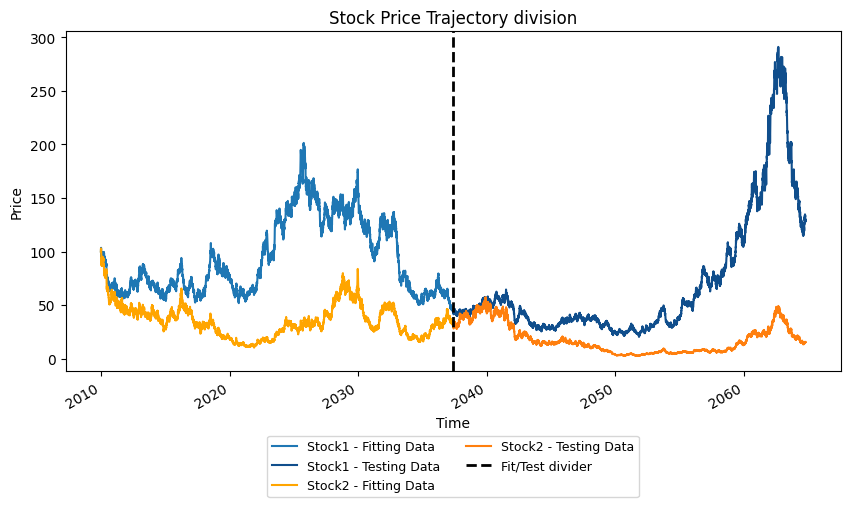
\includegraphics[width=0.8\textwidth]{4Method/pictures/DataDivision.png}
\caption{Illustration of how the data is divided into fitting and testing parts.}
\label{fig:DataDivision}
\end{figure}

An example comparison between the test data and data generated from a fitted copula is shown in \Cref{fig:TestSampleComparison}. The red points represent test data from a Clayton copula, while the blue points are samples from a fitted Gaussian copula. If the copula successfully captures dependency, the two distributions should be visually and statistically similar.

\begin{figure}
\centering
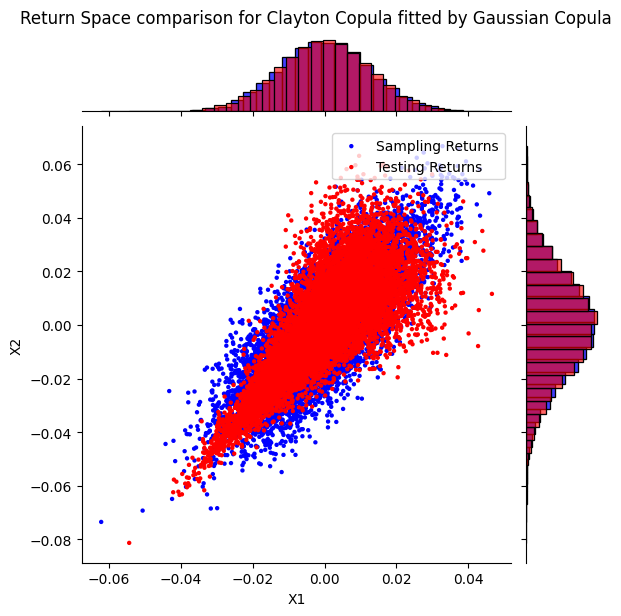
\includegraphics[width=0.5\textwidth]{4Method/pictures/TestSampleComparison.png}
\caption{Comparison between test data and data sampled from a fitted copula.}
\label{fig:TestSampleComparison}
\end{figure}

To evaluate the copulas’ ability to model dependency accurately, it is necessary to compare the generated and test datasets. Simulated data is used to ensure that the joint distribution remains stationary, satisfying the Monte Carlo assumption. If the copula-generated data closely resembles the test data, the dependency is well captured. Otherwise, it indicates the copula’s limitations.

It is important to emphasize that the core assumption behind using copulas for Monte Carlo simulation is that the joint distribution observed historically remains valid into the future.

To quantify the similarity between test and sampled data, the distance metric described in \Cref{sec:GoodnessOfFit} is used. This allows for calculating an average distance for each copula over multiple datasets and identifying the best-performing copula overall.

%%%%%%%%%%%%%%%%%%%%%%%%%%%%%%%%%%%%%%%%%%%%%%%%%%%%%%%%%%%%%%%%%%%%%%%%%%%%%
%%%% Marginal model test
%%%%%%%%%%%%%%%%%%%%%%%%%%%%%%%%%%%%%%%%%%%%%%%%%%%%%%%%%%%%%%%%%%%%%%%%%%%%%
\subsection{Marginal model test}
To validate the marginal model, a test is conducted to assess how closely the fitted marginal distribution matches the true distribution. This is done by generating data from known distributions and fitting the marginal model to it. The data is then transformed into probability space using the \gls{PIT}, both with the fitted and true distributions. The \gls{MAE} is computed to quantify the difference, and a QQ-plot is generated to visualize the fit.

Note that the generated data is subject to random noise, so the observed distribution may differ slightly from the true distribution, even though they are theoretically identical. Nevertheless, this test offers a good benchmark for how accurately the model fits marginals, providing a reference for what might be used if a neural network were not employed.

The tested distributions, along with their parameter values and descriptions, are shown in \Cref{tab:distributions}. For this test, all terms in the loss function defined in \Cref{sec:NeuralCopulaLoss} are equally weighted. Each distribution is tested using 10,000 data points.

\begin{table}[h]
    \centering
    \caption{Distributions and parameters used for the marginal model test.}
    \begin{tabular}{@{}ccl@{}}
        Distribution & Parameters & Description \\
        \toprule
        Gaussian & $\mu=0, \sigma=1$ & Standard normal distribution \\ 
        Student's $t$ & $\nu=5$ & Student's $t$-distribution with 5 degrees of freedom \\ 
        Uniform & $a=0, b=1$ & Uniform distribution on [0, 1] \\ 
        Exponential & $\lambda=1$ & Exponential distribution with rate 1 \\ 
        Laplace & $\mu=0, b=1$ & Laplace distribution with mean 0 and scale 1 \\ 
        Log-normal & $\mu=0, \sigma^2=1$ & Log-normal distribution with mean 0 and variance 1 \\ 
    \end{tabular}
    \label{tab:distributions}
\end{table}


%%%%%%%%%%%%%%%%%%%%%%%%%%%%%%%%%%%%%%%%%%%%%%%%%%%%%%%%%%%%%%%%%%%%%%%%%%%%%
%%%% Neural copula testing
%%%%%%%%%%%%%%%%%%%%%%%%%%%%%%%%%%%%%%%%%%%%%%%%%%%%%%%%%%%%%%%%%%%%%%%%%%%%%
\subsection{Neural Copula training scheme test}
This section outlines the procedure for identifying the best hyperparameters that produce a valid copula function. A copula is considered valid if it satisfies the conditions defined in \Cref{def:copula}. For the neural copula, this means that all loss terms—except the first—defined in \Cref{sec:NeuralCopulaLoss}, should approach zero after training.

To ensure robustness across datasets, the model will be tested on several datasets. For each dataset, a grid of hyperparameter values will be evaluated. These include solver type, learning rate, number of epochs, batch size, network architecture, and learning rate scheduler. This results in a large number of parameter combinations designed to identify a universally effective training setup. To keep runtime feasible, the grid is limited to 288\todo{Change} combinations, tested across five datasets using a computing cluster.

The datasets used for testing are listed in \Cref{tab:DatasetsTestedOn}, which specifies the copula, its parameters, and a dataset name for reference. The hyperparameter grid is summarized in \Cref{tab:se_hyperparams}. Parameters like "Network layers" and "Network neurons" define the \gls{NN} architecture, while "Learning rate", "Scheduler", and "Solver" relate to the optimization process. "Epochs" and "Batch size" govern training duration and granularity.

\begin{table}[h!]
    \centering
    \caption{Datasets used to test the neural copula hyper parameters and loss function weights.}
    \begin{tabular}{lll}
    \textbf{Copula} & \textbf{Parameter} & \textbf{Name}  \\
    \hline
    Gaussian & $\rho:0$ & Independece \\
    Gaussian & $\rho:0.7$ & Positive Dependece \\
    Gaussian & $\rho:-0.7$ & Negative Dependece  \\
    Gaussian & $\rho:0.999$ & Frechet Upper \\
    Gaussian & $\rho:-0.999$ & Frechet Lower \\
    \end{tabular}
    \label{tab:DatasetsTestedOn}
\end{table}

\begin{table}[h!]
    \centering
    \caption{Hyperparameter grid choices the test of the neural copula fitting procedure.}
    \begin{tabular}{ll}
    \textbf{Hyperparameter} & \textbf{Options} \\
    \hline
    Network layers & 2, 3, 4 \\
    Network neurons & 5, 10 \\
    Learning rate & 0.1, 0.01 \\
    Scheduler & step, exponential, None \\
    Solver & ADAM, SGD \\
    Epochs & 10000, 5000 \\
    Batch size & 1024, 2048 (Remove batch size) \\
    \end{tabular}
    \label{tab:se_hyperparams}
\end{table}

Each hyperparameter combination is evaluated using an ensemble of 10 runs to mitigate variability due to random initialization. The best run from each ensemble is selected for evaluation.

After testing all combinations, the best-performing setup across all datasets—measured by average loss—will be selected. If constraint-related loss terms are close to zero, the copula is considered valid. This best model is then used in the final experiment described in \Cref{sec:PortfolioTesting}.

Additionally, the effect of varying the weights of different loss function terms will be examined. While the first term is fixed to one, the other terms are scaled by 0.5, 1, and 2, respectively. The goal is to determine if emphasizing certain terms improves performance. This test uses the previously selected best hyperparameters, and evaluation is based on the equally weighted loss for fair comparison. Each copula from the hyperparameter test is included in this analysis to assess the effect of loss term weighting.


%%%%%%%%%%%%%%%%%%%%%%%%%%%%%%%%%%%%%%%%%%%%%%%%%%%%%%%%%%%%%%%%%%%%%%%%%%%%%%
%%%% Portfolio testing
%%%%%%%%%%%%%%%%%%%%%%%%%%%%%%%%%%%%%%%%%%%%%%%%%%%%%%%%%%%%%%%%%%%%%%%%%%%%%%
\subsection{Portfolio Testing}\label{sec:PortfolioTesting}
This section outlines the methodology used to evaluate copula models on synthetic financial portfolios with controlled dependence structures.

\subsubsection{Data Generation}
To assess the performance of different copulas, synthetic test portfolios of stock price data are generated. The aim is to isolate the role of the copula by ensuring consistent and known marginal distributions across all datasets, thereby preventing confounding effects from the marginal fitting process. As copulas are invariant under strictly increasing transformations (see \Cref{the:TranslationInvariance}), the choice of marginal distribution is arbitrary. In this study, standard normal distributions are used for all marginals.

Dependence is introduced via analytical copulas with varying parameters. Data is first sampled in probability space from the specified copulas. These samples are then transformed using the inverse CDF of the standard normal distribution, producing dependent samples with standard normal marginals. These samples are subsequently used as random shocks in simulating bivariate Geometric Brownian Motion (GBM) via the Euler-Maruyama scheme described in \Cref{sec:EulerMaruyama}.

This process yields synthetic price trajectories that reflect realistic financial behavior while preserving the controlled dependence introduced by the copula. The copulas and corresponding parameters used in the data generation process are summarized in \Cref{tab:DatasetsUsed}. Each simulation runs for 10,000 time steps (interpreted as trading days), with both assets having a drift of 0.03 and volatilities of 0.2 and 0.3, respectively.

\begin{table}[h!]
    \centering
    \caption{Portfolios used to evaluate the different copulas.}
    \begin{tabular}{ll}
    \textbf{Copula} & \textbf{Parameters} \\
    \hline
    Gaussian & Correlation: 0 \\
    Gaussian & Correlation: 0.7\\
    Student's $t$ & $\rho$: -0.8, $\nu$: 3\\
    Clayton & $\alpha$: 4 \\
    \end{tabular}
    \label{tab:DatasetsUsed}
\end{table}

The resulting datasets are visualized in \Cref{fig:DatasetsUsed}, which shows both the simulated price trajectories (left) and the log returns (right). Log returns are computed and partitioned into fitting (training) and testing datasets. The blue points represent fitting data used for model estimation, while the red points denote testing data used for performance evaluation. This mirrors a real-world setting where models are trained on historical data and evaluated on future, unseen data.

\begin{figure}
    \centering
    % --- (a) Independence ---
    \begin{minipage}{0.9\textwidth}
        \centering
        \begin{minipage}{0.54\textwidth}
            \centering
            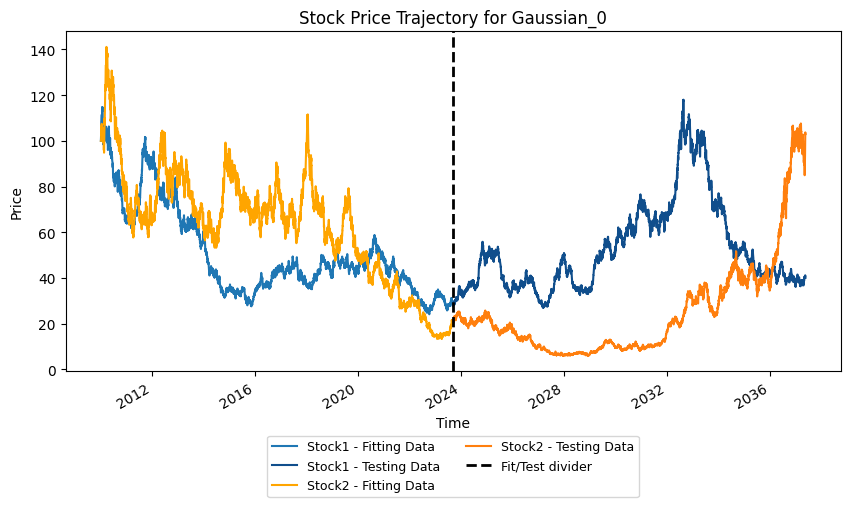
\includegraphics[width=\textwidth]{4Method/pictures/PricesGaussian_0.png}
        \end{minipage}
        \hfill
        \begin{minipage}{0.34\textwidth}
            \centering
            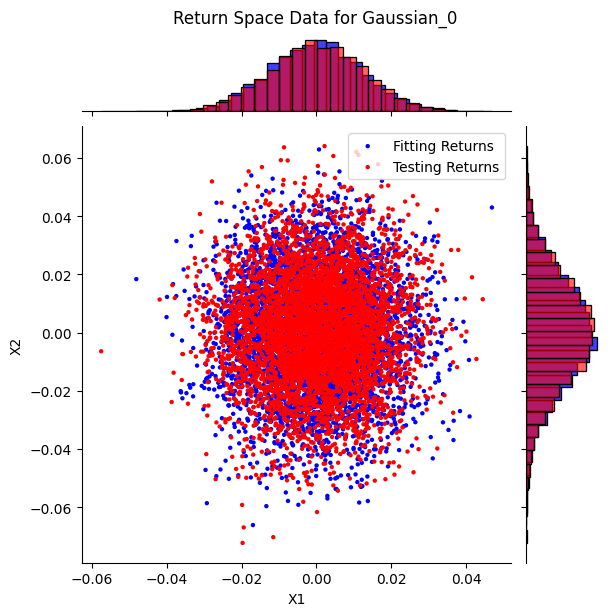
\includegraphics[width=\textwidth]{4Method/pictures/ReturnsGaussian_0.png}
        \end{minipage}
        \subcaption*{(a) Gaussian (independent)}
    \end{minipage}
    \hfill
    % --- (b) Student's t ---
    \begin{minipage}{0.9\textwidth}
        \centering
        \begin{minipage}{0.54\textwidth}
            \centering
            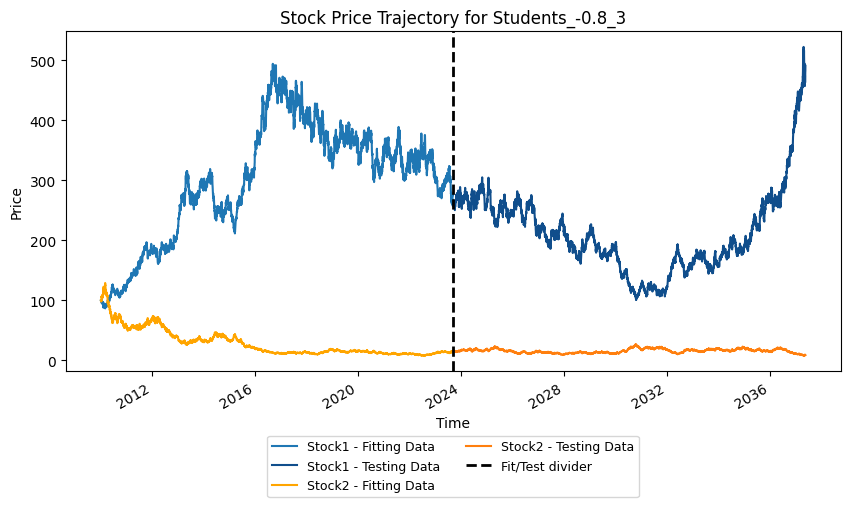
\includegraphics[width=\textwidth]{4Method/pictures/PricesStudents_-08_3.png}
        \end{minipage}
        \hfill
        \begin{minipage}{0.34\textwidth}
            \centering
            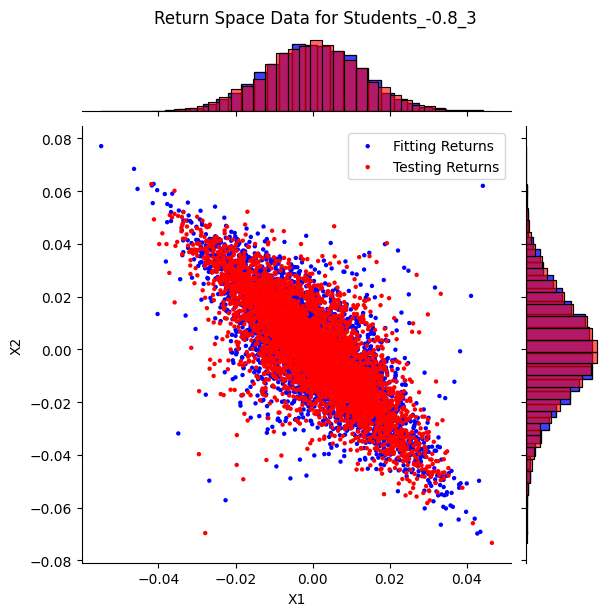
\includegraphics[width=\textwidth]{4Method/pictures/ReturnsStudents_-08_3.png}
        \end{minipage}
        \subcaption*{(b) Student's $t$ ($\rho = -0.8$, $\nu = 3$)}
    \end{minipage}
    \vfill
    % --- (c) Gaussian 0.7 ---
    \begin{minipage}{0.9\textwidth}
        \centering
        \begin{minipage}{0.54\textwidth}
            \centering
            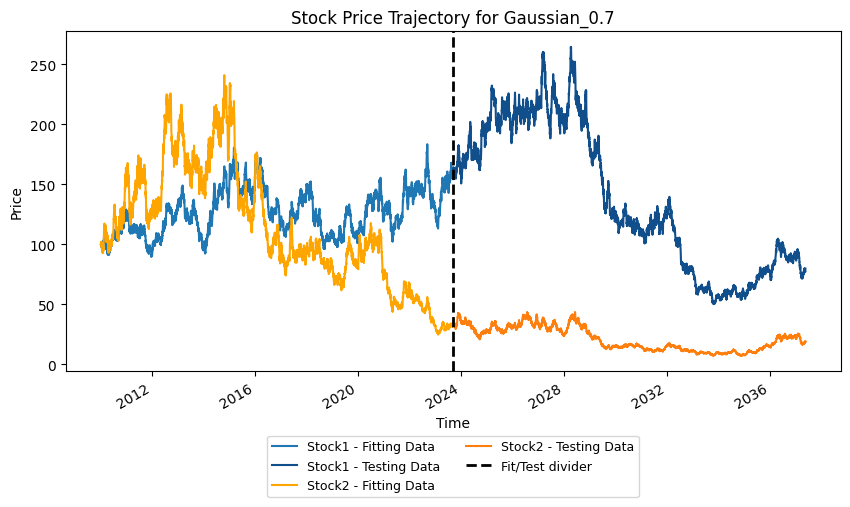
\includegraphics[width=\textwidth]{4Method/pictures/PricesGaussian_07.png}
        \end{minipage}
        \hfill
        \begin{minipage}{0.34\textwidth}
            \centering
            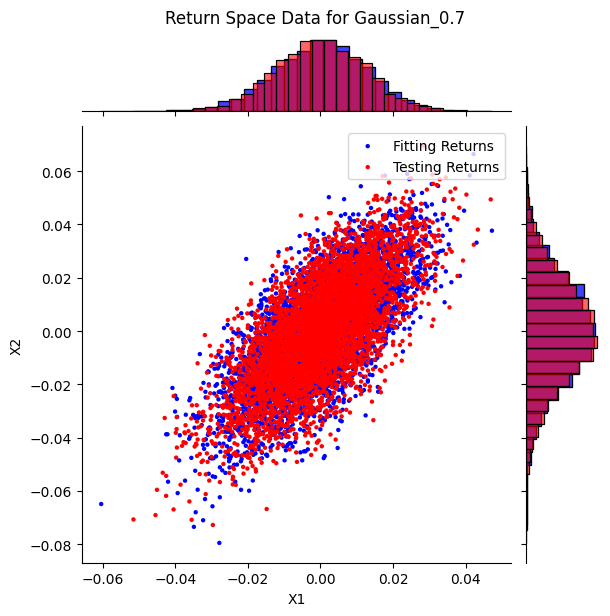
\includegraphics[width=\textwidth]{4Method/pictures/ReturnsGaussian_07.png}
        \end{minipage}
        \subcaption*{(c) Gaussian ($\rho = 0.7$)}
    \end{minipage}
    \hfill
    % --- (d) Clayton ---
    \begin{minipage}{0.9\textwidth}
        \centering
        \begin{minipage}{0.54\textwidth}
            \centering
            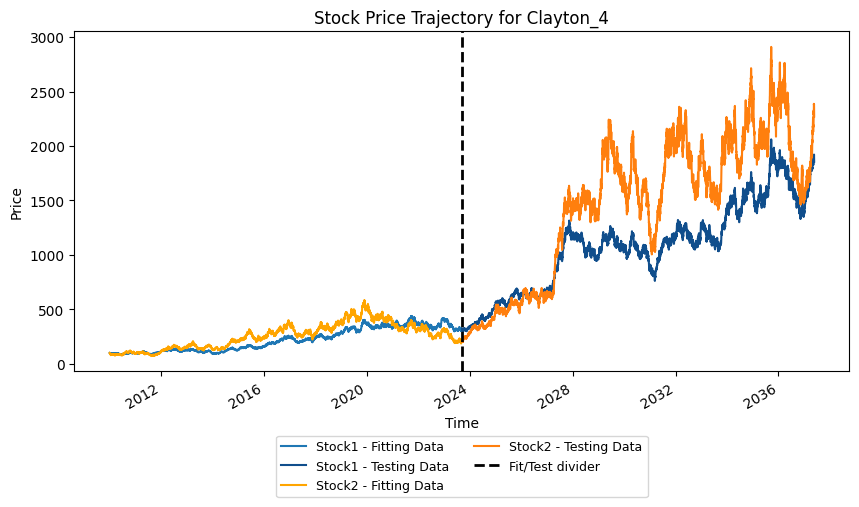
\includegraphics[width=\textwidth]{4Method/pictures/PricesClayton_4.png}
        \end{minipage}
        \hfill
        \begin{minipage}{0.34\textwidth}
            \centering
            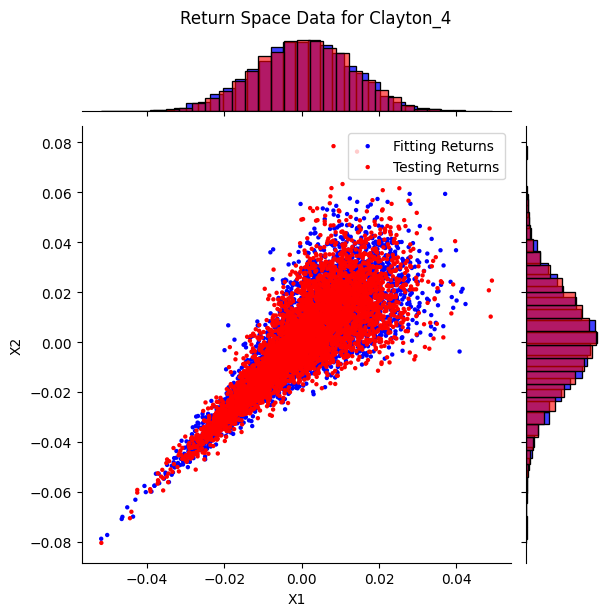
\includegraphics[width=\textwidth]{4Method/pictures/ReturnsClayton_4.png}
        \end{minipage}
        \subcaption*{(d) Clayton ($\alpha = 4$)}
    \end{minipage}
    \caption{Simulated test portfolios: Price trajectories (left) and corresponding log returns (right). Blue = fitting data, Red = testing data.}
    \label{fig:DatasetsUsed}
\end{figure}

\subsubsection{Model Fitting}
The log returns from the fitting portion of each dataset are first standardized to zero mean and unit variance. These normalized returns are then used to estimate the copula parameters. Fitting procedures follow the methods outlined in \Cref{sec:GaussianCopula} for the Gaussian copula, \Cref{sec:StudentsCopula} for the Student's $t$ copula, \Cref{sec:ClaytonCopula} for the Clayton copula, and \Cref{sec:NeuralCopulaFittingAndSampling} for the neural copula.


\subsubsection{Model Sampling}
A key use case for copulas is generating dependent samples for Monte Carlo simulations \citep[p.~40]{Nelsen2006}. Once fitted, each copula is used to sample new data in probability space. These samples are then mapped through the inverse normal CDF and scaled to match the empirical standard deviation of the original (fitting) data.

The neural copula, unlike the others, incorporates inverse marginal models directly and does not rely on the inverse normal transformation. If the copula accurately captures the dependence structure, the resulting synthetic data should closely resemble the testing dataset.

\subsubsection{Model Evaluation}
To evaluate performance, the sampled data from each fitted copula is compared to the corresponding testing data using the distance measure described in \Cref{sec:GoodnessOfFit}. For each copula, this distance is averaged across all datasets to yield an overall performance score. This facilitates a robust comparison of model quality across varying dependence structures.

\begin{generalinstructions}
    \begin{compactenum}
        \item Data Generation
        \begin{compactenum}
            \item Sample from copulas in probability space.
            \item Transform samples to standard normals.
            \item Use as random shocks in GBM simulations.
            \item Compute log returns and split into training/testing sets.
        \end{compactenum}
        \item Model Fitting (for each copula).
        \item Model Evaluation
        \begin{compactenum}
            \item Generate samples from each fitted copula.
            \item Compare to test data using distribution-based distance measures.
        \end{compactenum}
    \end{compactenum}
\end{generalinstructions}































%%%%%%%%%%%%%%%%%%%%%%%%%%%%%%%%%%%%%%%%%%%%%%%
%% Method before fixing using GPT
%%%%%%%%%%%%%%%%%%%%%%%%%%%%%%%%%%%%%%%%%%%%%%%

% This section explains and motivates the method used for the experiment tested in this thesis. First, we provide a summary of the method used, as this will help to give the overall procedure without getting stuck in the details. Then, a detailed description of each different part will be given in separate sections. 

% \begin{generalinstructions}
%     \begin{compactenum}
%         \item Method overview
%         \item Test of marginal model (does it deviate for some different distributions)
%         \item Choice of method for copula
%         \item Portfolio testing (Actual experiment)
%     \end{compactenum}
% \end{generalinstructions}


% %%%%%%%%%%%%%%%%%%%%%%%%%%%%%%%%%%%%%%%%%%%%%%%%%%%%%%%%%%%%%%%%%%%%%%%%%%%%%%%
% %%%% Method overview
% %%%%%%%%%%%%%%%%%%%%%%%%%%%%%%%%%%%%%%%%%%%%%%%%%%%%%%%%%%%%%%%%%%%%%%%%%%%%%%%
% \subsection{Method overview}
% This section describes the method used for the experiment. The method is divided into three main parts reflecting the different research questions. 

% \RQone was investigated by using a test of the marginal model is performed to see how well the marginal distributions are fitted. This is to see if the marginal distribution fitted by the marginal model works as intended. Theoretically there should not be any difference between the fitted marginal distribution and the true distribution of the data  given a sufficient number of samples. This is important as the copula is invariant to strictly increasing transformations, meaning that the fitted copula should be able to replicate the joint distribution of the data regardless of the marginal distributions used. In the main experiment we will know that the log returns are normally distributed. In reality this is not always the case, and therefore we want to test how well the \gls{NC} marginals works.

% The second part of the method investigates \RQtwo and consist of a test of what hyperparameter values makes the copula train the best. This is done by training several models with different hyperparameter values and choosing the parameters that result in the smallest loss. The goal of this part is to find parameter options works universally for the \gls{NC} meaning that the trained copula model produces a valid copula function that fits the data well. To do this the copulas will be trained on several different datasets to find make sure that the method works well regardless of the data. 

% The third part of the method is the main experiment that will answer \RQthree of this thesis and the overall procedure is as follows. To begin with, different portfolios with different types of dependency structures will be generated. This will be done by sampling data in probability space from different copulas and transforming it to return space using the \gls{ITM} to obtain dependent normally distributed returns, as described in \Cref{sec:CopulaUseCase}. This ensures that the marginal distributions of the created portfolios have normal marginal distributions, removing the need for fitting them in this experiment. This allows for an evaluation of the pure performance of the copula, without conflating it with potential errors from fitting marginal distributions. The generated normally distributed random numbers are then used as the random shocks from the Weiner process when simulating the \gls{GBM} using the Euler-Maruyama scheme to replicate stock price time series. This creates a realistic setting for when using copulas would be suitable.  

% The generated price time series are then divided into two different parts. These different parts represent the historical and the future returns of the portfolios. The splitting of data is illustrated in \Cref{fig:DataDivision} where the blue and orange lines are different simulated stocks over time. The price time series are divided at the dashed black line to create what we will call the fitting and testing parts. The fitting part is used for fitting the different copulas using historically observed data, the testing part can be considered the true distribution of future returns. As described when introducing \gls{MC} methods in \Cref{sec:MonteCarlo}, the key assumption is that of the statistical distribution of the data and that the distribution remains the same in the future. Hence the fitting part is used to fit the copulas to the historical data. From the fitted copula random numbers replicating the joint distribution is generated. If the copula adequately captures the dependence the generated data from the fitted copula should be similar to the future data. This is the main goal of this thesis, to evaluate how well different copulas can replicate the joint distribution of the data. An example of the what the different distributions can look like for the test data compared to the data sampled from the fitted copula can be viewed in \Cref{fig:TestSampleComparison} where the red data is the testing data from a Clayton copula that is to be replicated and the blue data is the data sampled from the fitted gaussian copula. If the copula captures the dependence well when fitted, these datasets should be similar. 

% \begin{figure}
%     \centering
%     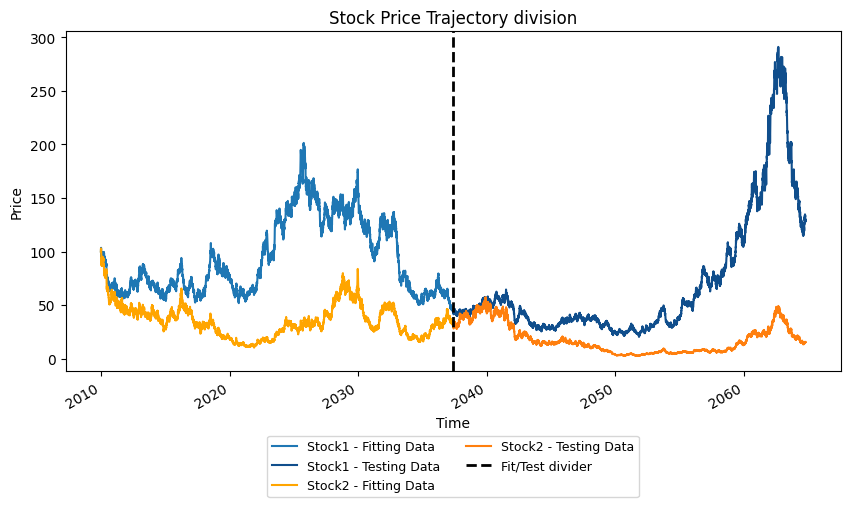
\includegraphics[width=0.8\textwidth]{4Method/pictures/DataDivision.png}
%     \caption{Illustration of how the data is divided into fitting and testing parts. }
%     \label{fig:DataDivision}
% \end{figure}

% \begin{figure}
%     \centering
%     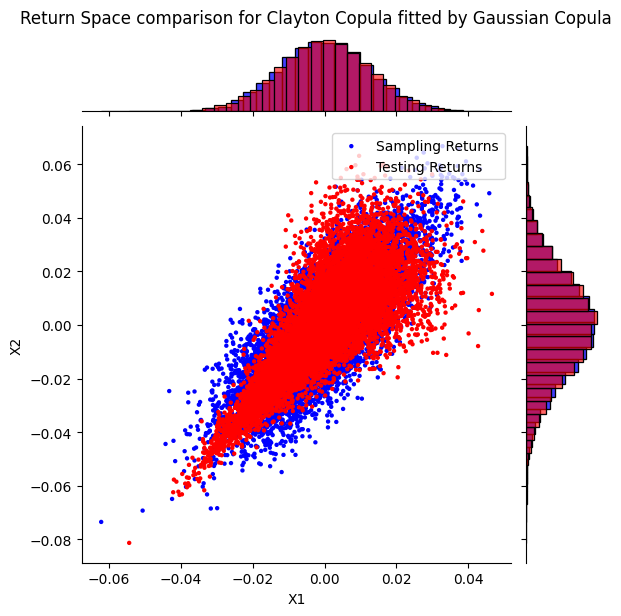
\includegraphics[width=0.5\textwidth]{4Method/pictures/TestSampleComparison.png}
%     \caption{Figure illustrating the difference between the test data and the data sampled from the fitted copula. }
%     \label{fig:TestSampleComparison}
% \end{figure}

% To evaluate the various copulas' ability to accurately capture the dependence between random variables, it is therefore sensible to compare the generated data to the testing data. The reason for using simulated data in this experiment is to ensure that the joint distribution is constant over time as this is a key assumption when using \gls{MC} methods. If the data generated from the fitted copula is similar to the testing data, it shows that the dependence is appropriately modeled by the copula. If not, it shows that the copula is not well suited to model the dependence. Hence this is a good way to evaluate the copulas' performance in an isolated manner. 

% To emphasize the key assumption when using copulas to simulate data for Monte Carlo purposes is that the joint distribution observed in the past continues to be the distribution from which the data is generated into the future. 

% To quantify how similar the test and sampled datasets are to each other, the distance measure described in \Cref{sec:GoodnessOfFit} is used. This allows for computing an average distance that each copula is from the test data over several datasets. This makes it possible to evaluate which copula performs best overall.  


% %%%%%%%%%%%%%%%%%%%%%%%%%%%%%%%%%%%%%%%%%%%%%%%%%%%%%%%%%%%%%%%%%%%%%%%%%%%%%
% %%%% Marginal model test
% %%%%%%%%%%%%%%%%%%%%%%%%%%%%%%%%%%%%%%%%%%%%%%%%%%%%%%%%%%%%%%%%%%%%%%%%%%%%%
% \subsection{Marginal model test}
% To validate that the marginal model works as intended, a test is performed to see how well the fitted marginal distribution matches the true distribution of the data. This is done by generating data from a known distribution and then fitting a marginal model to it. The fitted marginal model is then compared to the true distribution of the data by transforming the data to probability space using the \gls{PIT} using both the fitted distribution and the true distribution. To evaluate how similar the points in probability space are to each other the \gls{MAE} is calculated. Additionally a QQ-plot is created to visualize how well the fitted distribution matches how well the data follows the true distribution. During this experiment it is important to keep in mind that the generated data is subject to random noise, therefore it is not necessarily the case that the true distribution of the data is the exact same as the observed distribution even tough they should be. It is however a good benchmark to see how well the fitted distribution matches the true distribution, which would be a reasonable choice of distribution to use if the neural network was not used. The distributions used for the test are listed in \Cref{tab:distributions} where the distribution, the parameter values, and a short description is displayed for each of the tested distributions. In this test the different terms of the loss function defined in \Cref{sec:NeuralCopulaLoss} are equally weighted. The number of data points used for each distribution is 10000.

% \begin{table}[h]
%     \centering
%     \caption{Distributions and parameters used for the marginal model test.}
%     \begin{tabular}{@{}ccl@{}}
%         Distribution & Parameters & Description \\
%         \toprule
%         Gaussian & $\mu=0, \sigma=1$ & Standard normal distribution \\ 
%         Student's $t$ & $\nu=5$ & Student's $t$-distribution with 5 degrees of freedom \\ 
%         Uniform & $a=0, b=1$ & Uniform distribution on [0, 1] \\ 
%         Exponential & $\lambda=1$ & Exponential distribution with rate 1 \\ 
%         Laplace & $\mu=0, b=1$ & Laplace distribution with mean 0 and scale 1 \\ 
%         Log-normal & $\mu=0, \sigma^2=1$ & Log-normal distribution with mean 0 and variance 1 \\ 
%     \end{tabular}
%     \label{tab:distributions}
% \end{table}



% %%%%%%%%%%%%%%%%%%%%%%%%%%%%%%%%%%%%%%%%%%%%%%%%%%%%%%%%%%%%%%%%%%%%%%%%%%%%%
% %%%% Neural copula testing 
% %%%%%%%%%%%%%%%%%%%%%%%%%%%%%%%%%%%%%%%%%%%%%%%%%%%%%%%%%%%%%%%%%%%%%%%%%%%%%
% \subsection{Neural Copula training scheme test}
% In this section the procedure for finding the best hyper parameters for the model to create a valid copula function is described. Wether or not a copula function is valid is determined by wether or not it satisfies the conditions of being a copula defined in \Cref{def:copula}. In practice for the neural copula this means that all but the first of the loss terms, defined in \Cref{sec:NeuralCopulaLoss}, should approach zero when training is done. Several different combinations of hyper parameters will be tested with the goal of some that work well, meaning that the fitted copula is valid.

% Several datasets will be used for testing the neural copula fitting procedure. This is to ensure that the method works well, regardless of the data, consistently resulting in valid copulas. The method for this workflow is as follows for each dataset. First different datasets will be generated and a grid of different parameter values will be created. The grid will contain different values for the parameters of the neural copula such as the solver used, learning rates, number of epochs, batch size, network architecture and step size scheduler. This creates a large number of different combinations of choices to test which will hopefully result in a method for finding a training method that works well universally. The number of alternatives tested in the grid is somewhat limited to make the execution time reasonable. In total 288\todo{Change} combinations of network parameters are tested for the five datasets. The test will be ran on a compute cluster but despite that the execution time will be long due to the large number of combinations. 

% The datasets that will be used for testing the neural copula fitting procedure are displayed in \Cref{tab:DatasetsTestedOn}. In the table the copula used to generate each dataset is stated along with parameter values. Additionally, the name of the dataset is stated for future reference. The hyper parameters that will be tested are displayed in \Cref{tab:se_hyperparams}. In the table we can see the hyper parameters Network layers and Network neurons that describe the architecture of the \gls{NN}. The parameters Learning rate, Scheduler and Solver describe the training procedure. The parameters Epochs and Batch size describe the training process. 

% \begin{table}[h!]
%     \centering
%     \caption{Datasets used to test the neural copula hyper parameters and loss function weights.}
%     \begin{tabular}{lll}
%     \textbf{Copula} & \textbf{Parameter} & \textbf{Name}  \\
%     \hline
%     Gaussian & $\rho:0$ & Independece \\
%     Gaussian & $\rho:0.7$ & Positive Dependece \\
%     Gaussian & $\rho:-0.7$ & Negative Dependece  \\
%     Gaussian & $\rho:0.999$ & Frechet Upper \\
%     Gaussian & $\rho:-0.999$ & Frechet Lower \\
%     \end{tabular}
%     \label{tab:DatasetsTestedOn}
% \end{table}

% \begin{table}[h!]
%     \centering
%     \caption{Hyperparameter grid choices the test of the neural copula fitting procedure.}
%     \begin{tabular}{ll}
%     \textbf{Hyperparameter} & \textbf{Options} \\
%     \hline
%     Network layers & 2, 3, 4 \\
%     Network neurons & 5, 10 \\
%     Learning rate & 0.1, 0.01 \\
%     Scheduler & step, exponential, None \\
%     Solver & ADAM, SGD \\
%     Epochs & 10000, 5000 \\
%     Batch size & 1024, 2048 (Remove batch size) \\
%     \end{tabular}
%     \label{tab:se_hyperparams}
% \end{table}\todo{Explain some options more}
    

% % For each of the combinations in the grid the an ensemble of runs will be performed to mitigate the impact of what random seeds are used for initializing the weights of the network. The ensemble will consist of 10 runs for each combination in the grid. The best run from the ensemble will be kept for each combination in the grid. 

% The different combinations of hyper parameters will be tested on each of the different datasets. After training the best overall method over the datasets, measured by the average loss, will be selected as the best one. If the losses relating to the copula function constraints close to zero. This indicates that the fitted copula is valid. The best model will be used in the final experiment, described in \Cref{sec:PortfolioTesting}.  

% As a further test, different weights will be used for the different terms in the loss function during training. This is to see what how big the different terms in the loss function should be in relation to each other. We fix the first term to be one, then 0.5, 1, and 2 is tested for the other terms. This test will be conducted using the best performing hyper parameters from the prior part of the test. The evaluation of this test will be done by looking at the equally weighted loss to make the comparison fair. This test is performed for each of the copulas used in the hyper parameter test. The idea of this test is to see if it can be beneficial to weight the different terms in the loss function differently in relation to each other to emphasize some terms in the loss function more. 

% % \begin{generalinstructions}
% % Given generated datasets and a specified grid\\
% % \textbf{For each dataset}
% % \begin{compactitem}
% %     \item \textbf{For grid alternative}
% %     \begin{compactitem}
% %             \item Train copula on dataset
% %         \end{compactitem}
% % \end{compactitem}
% % \textbf{Evaluate the average performance of methods over the datasets}
% % \end{generalinstructions}
 
% \todo{How have i changed the neural copula approach, errors in the neural copula article.}


% %%%%%%%%%%%%%%%%%%%%%%%%%%%%%%%%%%%%%%%%%%%%%%%%%%%%%%%%%%%%%%%%%%%%%%%%%%%%%%
% %%%% Portfolio testing
% %%%%%%%%%%%%%%%%%%%%%%%%%%%%%%%%%%%%%%%%%%%%%%%%%%%%%%%%%%%%%%%%%%%%%%%%%%%%%%
% \subsection{Portfolio testing}\label{sec:PortfolioTesting}
% This section details the steps in the test of the copulas on the different portfolios. 

% \subsubsection{Data Generation}
% To evaluate the performance of different copulas when fitted to data we need data to test the copulas on. The data comes in the form of test portfolios of artificially generated stock price data given that this thesis focuses on the use of copulas in modelling financial returns. These portfolios should ideally cover a wide range of dependence structure types. This is to test the different copulas' versatility and robustness under varying conditions. 

% This thesis focuses on the role of the copula purely and therefore, the aim is not to conflate the results from the copula's performance with that of the marginal fitting procedure. Therefore, we want each marginal distribution of the generated portfolios to be the same known distribution, removing the need for fitting the marginal distributions. The marginal distributions used should not matter, given that the copula is invariant to strictly increasing transformations as stated in \Cref{the:TranslationInvariance}. In this study the marginal distributions used will be the normal distribution. If having different marginal distributions the number of combinations to test during model fitting becomes large. 

% To generate portfolios with different dependence structures and the same marginal distributions, copulas will be used. This will be done by first sampling data from analytical copulas with different parameter values. The result will be data points in probability space that contain the pure dependence between the different variables. These data points will then be plugged into the inverse \gls{CDF} of a Standard normal distribution. This performs the \gls{PIT} in reverse, creating data points with standard normal marginal distributions with the dependence described by the copula. 

% After having generated these pairs of dependent standard, normally distributed random numbers, they are used as the random shocks when simulating the bivariate \gls{GBM} using the Euler-Maruyama scheme defined in \Cref{sec:EulerMaruyama}. This results in test portfolios representing stock prices over time, creating a realistic setting for when using copulas is appropriate. 

% The above procedure for generating data is used for the copulas specified in \Cref{tab:DatasetsUsed}. In the table we can see the different copulas and the parameter values for them. The stock trajectories are simulated for 10000 time periods representing days. Both stocks have a drift term of 0.03 and the volatility is set to 0.2 and 0.3 for stock one and two respectively. 
% \begin{table}[h!]
%     \centering
%     \caption{Portfolios used to evaluate the different copulas.}
%     \begin{tabular}{ll}
%     \textbf{Copula} & \textbf{Parameters} \\
%     \hline
%     Gaussian & Correlation: 0 \\
%     Gaussian & Correlation: 0.7\\
%     Students $t$ & $\rho$: -0.8, $\nu$: 3\\
%     Clayton & Alpha: 4 \\
%     \end{tabular}
%     \label{tab:DatasetsUsed}
% \end{table}

% The resulting portfolios can be observed in \Cref{fig:DatasetsUsed} where the left pictures show the price time series of the different portfolios and the right pictures show the log returns of the portfolios. In the left pictures we can see how the portfolios are divided over time. In the right pictures we can see the log returns of the portfolios. The blue points show the log returns of the fitting data and the red points show the log returns of the testing data. The fitting part will be used in the model fitting and can be thought of as historically observed data. The testing part will be used in the model evaluation and can be thought of as data that will appear in the future, which we want to replicate as well as possible by sampling from a copula fitted to the historical data. 

% \begin{figure}
%     \centering
%     % --- (a) Independence ---
%     \begin{minipage}{0.9\textwidth}
%         \centering
%         \begin{minipage}{0.54\textwidth}
%             \centering
%             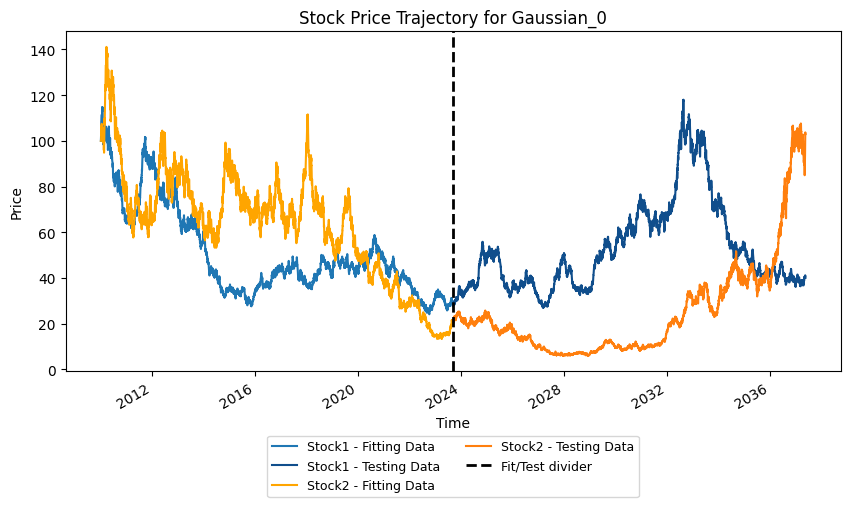
\includegraphics[width=\textwidth]{4Method/pictures/PricesGaussian_0.png}
%             %\subcaption*{Histogram}
%         \end{minipage}
%         \hfill
%         \begin{minipage}{0.34\textwidth}
%             \centering
%             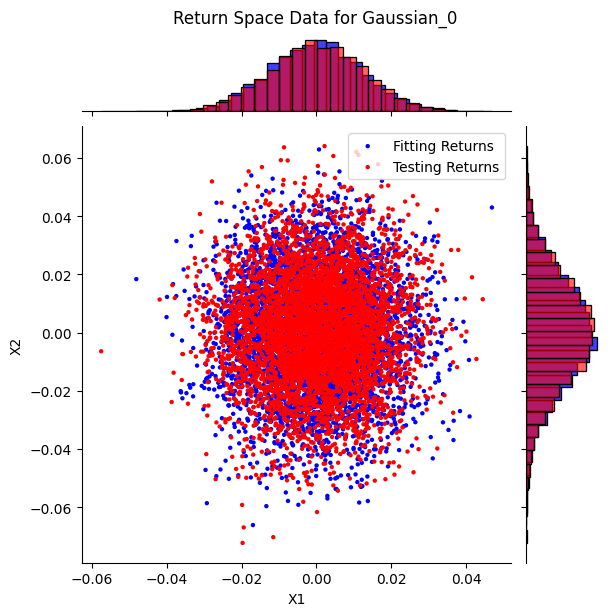
\includegraphics[width=\textwidth]{4Method/pictures/ReturnsGaussian_0.png}
%             %\subcaption*{QQ plot}
%         \end{minipage}
%         \subcaption*{(a) Independent}
%     \end{minipage}
%     \hfill
%     % --- (b) Student's t ---
%     \begin{minipage}{0.9\textwidth}
%         \centering
%         \begin{minipage}{0.54\textwidth}
%             \centering
%             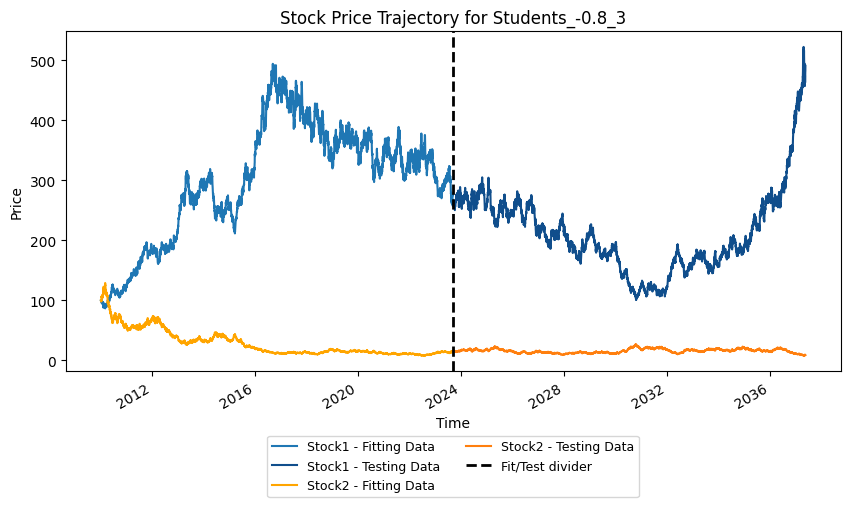
\includegraphics[width=\textwidth]{4Method/pictures/PricesStudents_-08_3.png}
%             %\subcaption*{Histogram}
%         \end{minipage}
%         \hfill
%         \begin{minipage}{0.34\textwidth}
%             \centering
%             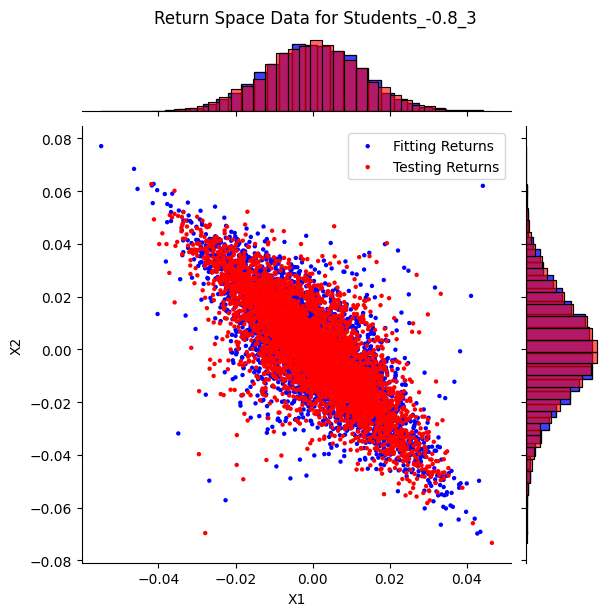
\includegraphics[width=\textwidth]{4Method/pictures/ReturnsStudents_-08_3.png}
%             %\subcaption*{QQ plot}
%         \end{minipage}
%         \subcaption*{(b) Student's $t$ -0.8 3}
%     \end{minipage}
%     \vfill
%     % --- (c) gaussian 0.7 ---
%     \begin{minipage}{0.9\textwidth}
%         \centering
%         \begin{minipage}{0.54\textwidth}
%             \centering
%             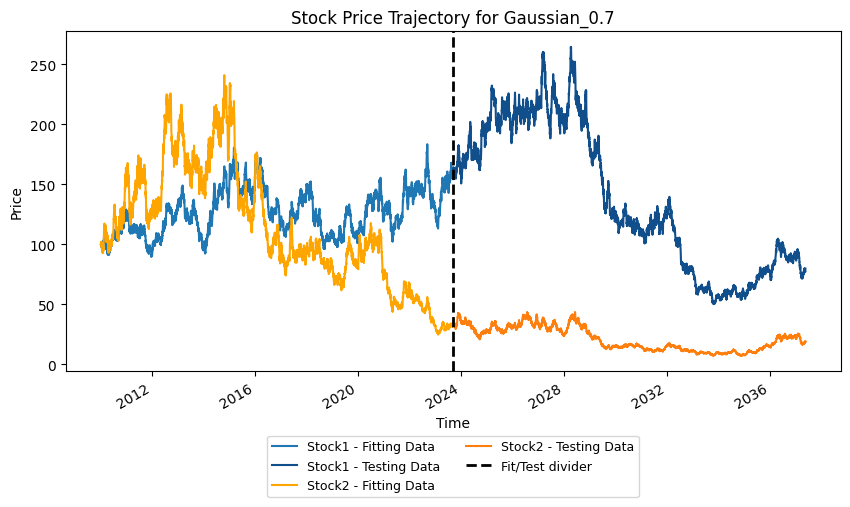
\includegraphics[width=\textwidth]{4Method/pictures/PricesGaussian_07.png}
%             %\subcaption*{Histogram}
%         \end{minipage}
%         \hfill
%         \begin{minipage}{0.34\textwidth}
%             \centering
%             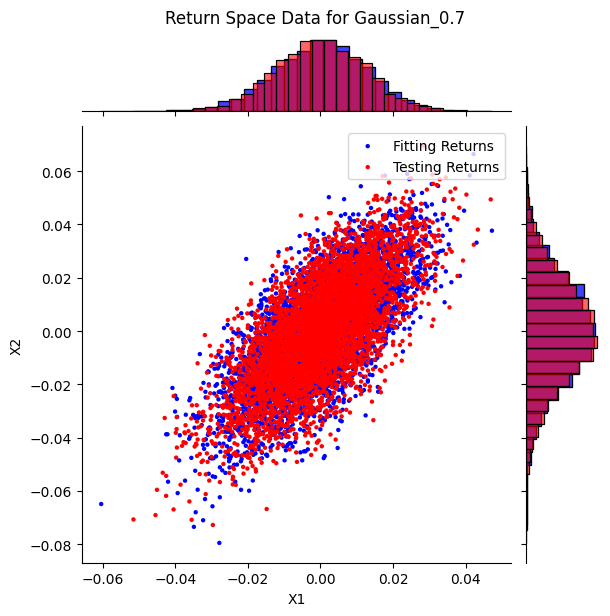
\includegraphics[width=\textwidth]{4Method/pictures/ReturnsGaussian_07.png}
%             %\subcaption*{QQ plot}
%         \end{minipage}
%         \subcaption*{(c) Gaussian 0.7}
%     \end{minipage}
%     \hfill
%     % --- (d) Clayton ---
%     \begin{minipage}{0.9\textwidth}
%         \centering
%         \begin{minipage}{0.54\textwidth}
%             \centering
%             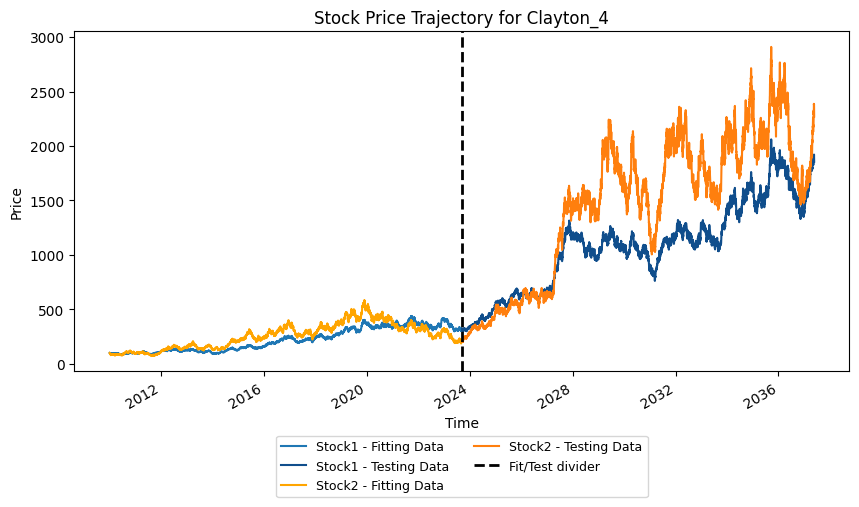
\includegraphics[width=\textwidth]{4Method/pictures/PricesClayton_4.png}
%             %\subcaption*{Histogram}
%         \end{minipage}
%         \hfill
%         \begin{minipage}{0.34\textwidth}
%             \centering
%             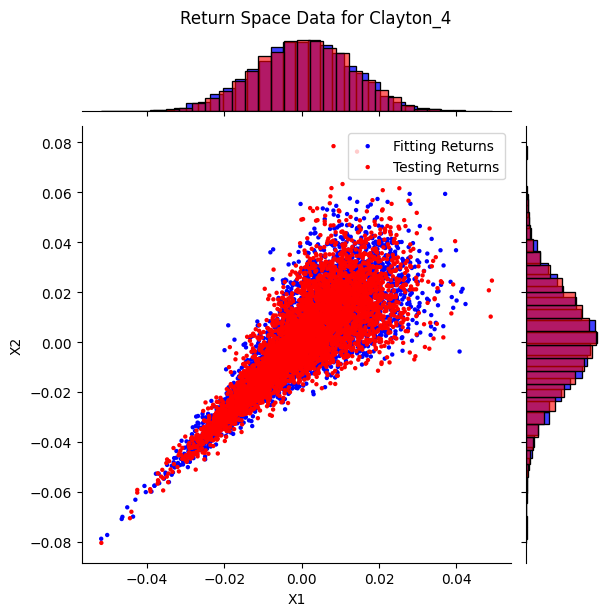
\includegraphics[width=\textwidth]{4Method/pictures/ReturnsClayton_4.png}
%             %\subcaption*{QQ plot}
%         \end{minipage}
%         \subcaption*{(d) Clayton 4}
%     \end{minipage}
%     \caption{Figure displaying the test portfolios price series and log returns for the portfolio test.}
%     \label{fig:DatasetsUsed}
% \end{figure}


% \subsubsection{Model Fitting}
% The fitting data from each of the previously generated portfolios is used for fitting the different copulas. To do this, the data needs to be converted so that the copulas can work with it. Hence, the log returns are calculated as defined in \Cref{def:logReturns}. These are then standardized and centered to have a zero mean and unit variance. 

% The different types of copulas are then fitted as described for the Gaussian in \Cref{sec:GaussianCopula}, the Student's $t$ in \Cref{sec:StudentsCopula}, the Clayton in \Cref{sec:ClaytonCopula} and the \gls{NC} in \Cref{sec:NeuralCopulaFittingAndSampling}. 


% \subsubsection{Model Sampling}
% The main use for copulas is arguably to sample random numbers to be used in \gls{MC} simulations \Citet[p.~40]{Nelsen2006}. The random numbers from the copula can be used to generate dependent realizations of a pair of random variables, regardless of their marginal distributions. Hence, it should make sense to evaluate the copulas based on how well generated random numbers from a fitted copula replicates the true dependence structure of the data. The procedures for sampling from the copulas is described for the Gaussian in \Cref{sec:GaussianCopula}, the Student's $t$ in \Cref{sec:StudentsCopula}, the Clayton in \Cref{sec:ClaytonCopula} and the \gls{NC} in \Cref{sec:NeuralCopulaFittingAndSampling}. 

% The sampled data points from the copulas, other than the \gls{NC} which uses the inverse marginal models, are inserted into the inverse normal distribution and then scaled to match the observed standard deviation of the fitting data. This should generate data similar to the data in the testing part if the copula adequately captures the dependence in the data.

% \subsubsection{Model evaluation}
% To evaluate the performance of each copula for each of the datasets the distance measure described in \Cref{sec:GoodnessOfFit} is used. An average of the distance measure is calculated over the different datasets for each copula. This will give a good indication of how well each copula performs overall. 





% \begin{generalinstructions}
%     \begin{compactenum}
%         \item Data generation
%         \begin{compactenum}
%             \item Generate returns
%             \item Put into GBM as random shocks 
%             \item Calculate log returns 
%             \item Split into different parts (train - test)
%         \end{compactenum}
%         \item Model fitting (for each copula)
%         \item Model evaluation
%         \begin{compactenum}
%             \item Compare the data generated by each copula on distribution level to the testing data for the different datasets
%         \end{compactenum}
%     \end{compactenum}
% \end{generalinstructions}




%%%%%%%%%%%%%%%%%%%%%%%%%%%%%%%%%%%%%%%%%%%%%%%%%%%%%%%%%%%%%%%%%%%%%%%%%%%%%%%%%%%%%%%%%%%
%% Results and Discussion 
%%%%%%%%%%%%%%%%%%%%%%%%%%%%%%%%%%%%%%%%%%%%%%%%%%%%%%%%%%%%%%%%%%%%%%%%%%%%%%%%%%%%%%%%%%%
\section{Results and Discussion}\label{sec:Results}
This section presents the results of the tests conducted on the simulated data. The tests include the marginal model test, the neural copula test, and the portfolio test, defined in \Cref{sec:Method}.

\subsection{Marginal Model Test}
The losses of the models in the marginal model test after training is shown in \Cref{tab:MarginalFinalLosses}. The table shows the total loss and the losses for each of the four terms in the loss function. The total loss is the sum of the four terms. The loss terms L2, L3, and L4 are the losses governed by constraints whereas L1 is the term maximizing the likelihood of the observed data. 

We can see that constraint losses are very close to zero for all distributions, indicating that the models satisfy the constraints. In \Cref{fig:MarginalResults}, we show the trained \gls{CDF} in a plot together with its corresponding \gls{PDF} and the observed data in a histogram. The generated QQ plots all show a perfect straight line and hence the inclusion of these plots is omitted. Visually it seems like the fitted models are able to capture the true distributions well. The most difficult distribution to fit seems to be the uniform distribution which has a somewhat unstable \gls{PDF}, this is also reflected in the total loss being the greatest. Overall, all distributions seem to be fitted well, and the QQ plots indicate that the transformed data is very similar regardless of whether using the fitted model or the true distribution. The conclusion is that the marginal model seem to be able to adequately fit a wide range of distributions. The results of the marginal model test answer the first research question \RQone about if the marginal models are adequate for the task of fitting the marginal distributions. The answer to this question is yes as the models are able to fit the distributions well. These results are limited to the distributions tested and the data used. The models may not perform as well on other distributions or datasets. There is however, nothing in these results suggesting that the results would not hold. The results are partly influenced by randomness since the distributions are randomly sampled and the model weights are also randomized. These results are in line with the results of \Citet[FindPage]{ZengWang2022}. What would be interesting to see is how to best work around the requirement of having to normalize the data before training the marginal models. This becomes especially relevant when trying to fit distributions that accurately capture the tails of the distribution where observations are rare.  


\begin{table}[h]
    \centering
    \caption{Losses for the trained marginal models after training for each distribution.}
    \begin{tabular}{llllll}
        Distribution & Total Loss & L1 & L2 & L3 & L4 \\
        \midrule
        Gaussian & -0.610431 & -0.6109432 & 0.0 & 0.00030577183 & 0.000206 \\
        Student-t & -1.700450 & -1.7008212 & 0.0 & 0.00023537874 & 0.000135 \\
        Uniform & 0.002953 & 0.0013246911 & 0.0 & 0.0008457899 & 0.000782 \\
        Exponential & -1.148577 & -1.1511308 & 0.0 & 0.0011827946 & 0.001371 \\
        Laplace & -1.196009 & -1.1963692 & 0.0 & 0.00022995472 & 0.000130 \\
        LogNormal & -2.257325 & -2.2578392 & 0.0 & 0.0002965927 & 0.000218 \\
    \end{tabular}
    \label{tab:MarginalFinalLosses}
\end{table}


\begin{figure}
    % --- (a) Normal ---
        \begin{minipage}{0.45\textwidth}
            \centering
            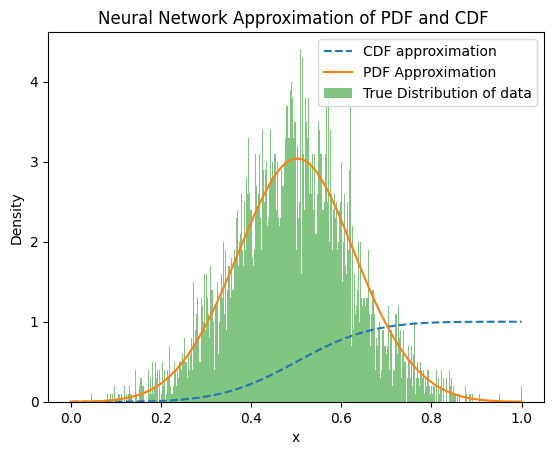
\includegraphics[width=\textwidth]{5ResultsDiscussion/pictures/MarginalTest/NormalHistogram.png}
            \subcaption*{(a) Normal}
        \end{minipage}
    \hfill
    % --- (b) Student's t ---
        \begin{minipage}{0.45\textwidth}
            \centering
            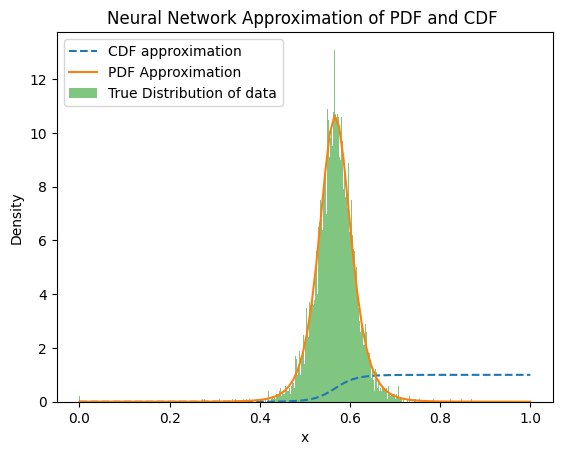
\includegraphics[width=\textwidth]{5ResultsDiscussion/pictures/MarginalTest/StudentsHistogram.png}
            \subcaption*{(b) Student's t}
        \end{minipage}

    \vspace{1em}

    % --- (c) Uniform ---
        \begin{minipage}{0.45\textwidth}
            \centering
            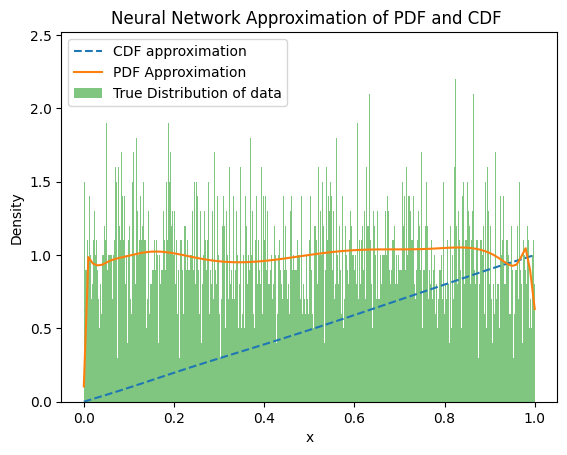
\includegraphics[width=\textwidth]{5ResultsDiscussion/pictures/MarginalTest/UniformHistogram.png}
            \subcaption*{(c) Uniform}
        \end{minipage}
    \hfill
    % --- (d) Exponential ---
        \begin{minipage}{0.45\textwidth}
            \centering
            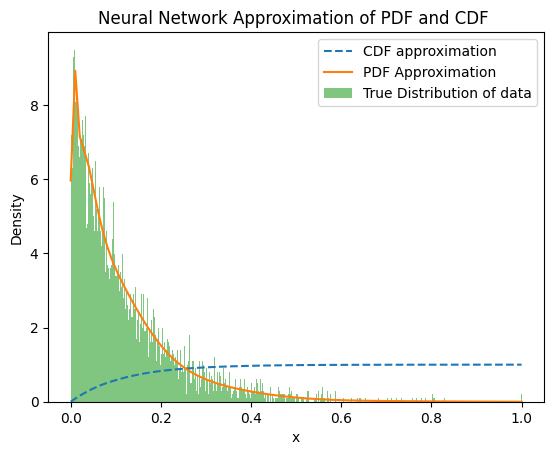
\includegraphics[width=\textwidth]{5ResultsDiscussion/pictures/MarginalTest/ExponentialHistogram.png}
            \subcaption*{(d) Exponential}
        \end{minipage}

    \vspace{1em}

    % --- (e) Laplace ---
        \begin{minipage}{0.45\textwidth}
            \centering
            \includegraphics[width=\textwidth]{5ResultsDiscussion/pictures/MarginalTest/LaplaceHistogram.png}
            \subcaption*{(e) Laplace}
        \end{minipage}
    \hfill
    % --- (f) Lognormal ---
        \begin{minipage}{0.45\textwidth}
            \centering
            \includegraphics[width=\textwidth]{5ResultsDiscussion/pictures/MarginalTest/LognormalHistogram.png}
            \subcaption*{(f) Lognormal}
        \end{minipage}

    \caption{Marginal distribution visualizations. Each subfigure (a--f) shows a histogram with the trained model for the distribution.}
    \label{fig:MarginalResults}
\end{figure}


%%%%%%%%%%%%%%%%%%%%%%%%%%%%%%%%%%%%%%%%%%%%%%%%%%%%%%
%% Neural Copula Test   
%%%%%%%%%%%%%%%%%%%%%%%%%%%%%%%%%%%%%%%%%%%%%%%%%%%%%%
\subsection{Neural Copula Test}
The results of the grid search for the hyperparameters and weights are shown in \Cref{tab:Best_hyperparams} and \Cref{tab:Best_weights} respectively. Additionally, the losses for the different datasets using the best hyper parameters and weights are shown in \Cref{tab:LossesBestParameters}. These hyperparameter options answer the second research question \RQtwo about how to train the \gls{NC} to obtain the best results. The observations from these results are that the best performing hyperparameters are a network with three layers and ten neurons in each layer. The learning rate is 0.1 and the solver is Adam. The best performing scheduler is exponential and the number of epochs is 10000. 

\begin{table}[h!]
    \centering
    \caption{The best choice of hyper parameters found in the grid search.}
    \begin{tabular}{ll}
    \textbf{Hyperparameter} & \textbf{Options} \\
    \hline
    Network layers & 3 \\
    Network neurons & 10 \\
    Learning rate & 0.1 \\
    Scheduler & exponential \\
    Solver & Adam \\
    Epochs & 10000 \\
    Batch size & 2048 (Not valid, should remove this as dataset was smaller)\\
    \end{tabular}
    \label{tab:Best_hyperparams}
\end{table}
    
\begin{table}[h!]
    \centering
    \caption{The best choice of weights found for the copula loss function linear combination defined in \Cref{sec:NeuralCopulaLoss}.}
    \begin{tabular}{ll}
    \textbf{Weight} & \textbf{Options} \\
    \hline
    $\lambda_1$ & 1 \\
    $\lambda_2$ & 2 \\
    $\lambda_3$ & 0.5 \\
    $\lambda_4$ & 1 \\
    $\lambda_5$ & 1 \\
    \end{tabular}
    \label{tab:Best_weights}
\end{table}
    

    
\begin{table}[h!]
    \centering
    \caption{Losses for the datasets using the best hyper parameters and weights.}
    \begin{tabular}{lllllll}
        \textbf{Dataset} & \textbf{L1}& \textbf{L2}& \textbf{L3}& \textbf{L4}& \textbf{L5}& \textbf{Total Loss} \\
        \midrule
        Independent & 0.065705 & 0.025223 & 0.045032 & 0.077263 & 0.005574 & 0.218797 \\
        PositiveDependence & 0.290332 & 0.033420 & 0.049284 & 0.239172 & 0.017931 & 0.630140 \\
        NegativeDependence & -0.281669 & 0.025645 & 0.047584 & 0.082656 & 0.005116 & -0.120667 \\
        FrechetUpper & -3.846874 & 0.095704 & 0.257008 & 0.122417 & 0.014359 & -3.357385 \\
        FrechetLower & -3.611439 & 0.080854 & 0.000004 & 0.108494 & 0.003596 & -3.418491 \\
        \end{tabular}
    \label{tab:LossesBestParameters}
\end{table}

\begin{remark}
    When testing to rerun the training of the \gls{NC} for the different datasets a numerical instability was encountered. This sometimes results in that the copula does not train properly and that the loss function does not converge to zero for the constraint terms. In the cases where this was encountered the resulting copula surface did not look remotely like a copula function. 
\end{remark}

These results are limited to the datasets used in this test and the hyperparameters tested. The results may not be generalizable to other datasets or hyperparameters particularly when the dimensionality of the data increases. The results could also be influenced by the numerical instability observed during training. To be more certain about the results, it would be a good idea to test running this test with more hyperparameters, weights, and to run each training of the copulas several times to see which hyperparameters are truly the most reliable. This was not done in this thesis due to the large amount of time this would take to run. Given that this is a new method there is not much previous research to compare the results to. We must also mention that the results are influenced by randomness since the datasets are randomly sampled and the model weights are also randomized. 


%%%%%%%%%%%%%%%%%%%%%%%%%%%%%%%%%%%%%%%%%%%%%%%%%%%%%
%% Portfolio Test
%%%%%%%%%%%%%%%%%%%%%%%%%%%%%%%%%%%%%%%%%%%%%%%%%%%%%
\subsection{Portfolio Test}
The results of the portfolio test are shown in \Cref{tab:DistributionDistances}. In the table, the distance between the data generated using the fitted copula and the true distribution is shown. The distance is calculated as described in \Cref{sec:GoodnessOfFit}. The last row in the table shows the total distance over all datasets for each copula used for fitting. This shows that the Gaussian copula was the best performing copula overall for the tested datasets. The order of the remaining copulas is as follows: Clayton, Neural, and Students $t$. Of particular interest is the performance of the \gls{NC}. It seems like the \gls{NC} is not able to fit the data better than the other copulas which \RQthree was asking. The fact that the Gaussian copula performed the best in this test should not be seen as a justification for using the Gaussian copula in practice. It is the result of this experiment but does not mean that the Gaussian copula is the best generally speaking. As an example, an article in Financial Times \footnote{See \url{https://www.ft.com/content/912d85e8-2d75-11de-9eba-00144feabdc0}. Sam Jones. The formula that felled Wall St. Financial Times. 24-04-2009. Last Accessed 2025-05-15.} explains how the Gaussian copula was used to model the dependence between mortgage backed securities which is said to have been a contributing factor to the financial crisis of 2008.  

\begin{table}[h!]
    \centering
    \caption{Distance between the fitted copula and the true distribution for the different distributions. The distance is calculated as described in \Cref{sec:GoodnessOfFit}.}
    \begin{tabular}{lllll}
    \textbf{Dataset/Copula} & \textbf{Gaussian} & \textbf{Students} & \textbf{Clayton} & \textbf{Neural} \\
    \hline
    % Gaussian, $\rho$: 0 & 0.00036880264225801646 & 0.0038564860944720883 & 0.00025453304967998163 & 0.002076942666237979 \\
    % Gaussian, $\rho$: 0.7 & 0.0005745609625385594 & 0.003405384070244613 & 0.0010251930676579886 & 0.0026765474087561796 \\
    % Students $t$, $\rho$: -0.8, $\nu$: 3 & 0.0005848558576855685 & 0.0013683433848652698 & 0.004119685177811808 & 0.0008999958003606833 \\
    % Clayton, $\alpha$: 4 &  0.0012345696582828495 & 0.0011805210541269663 & 0.001246438499213834 & 0.0026185757619811086 \\
    % Total & 0.0027627891207649942 & 0.009876652048795806 & 0.0038945080014170744 & 0.00827206163733595 \\
    Gaussian, $\rho$: 0               & 0.000369 & 0.003856 & 0.000255 & 0.002077 \\
    Gaussian, $\rho$: 0.7             & 0.000575 & 0.003405 & 0.001025 & 0.002677 \\
    Students $t$, $\rho$: -0.8, $\nu$: 3 & 0.000585 & 0.001368 & 0.004120 & 0.000900 \\ 
    Clayton, $\alpha$: 4              & 0.001235 & 0.001181 & 0.001246 & 0.002619 \\ %done
    \textbf{Total}      & \textbf{0.002764} & \textbf{0.009810} & \textbf{0.006646} & \textbf{0.008273} \\
    \end{tabular}
    \label{tab:DistributionDistances}
\end{table}

To better understand the results of the portfolio test, we investigate the data that the fitted copulas have generated. The data generated from the portfolio having dependence specified by a Clayton copula with $\alpha=4$ is shown in \Cref{fig:GeneratedDataClayton}. The figure shows the generated from each copula after being fitted to the data. We can see that it is only the clayton copula that is able to generate data that looks like the true distribution. Both the gaussian and the students $t$ are unable to capture the behavior of the data in the lower tail and hence the generated data looks very different from the true distribution. The \gls{NC} does seem to partially capture the behavior of the data by having a slightly pointy shape in the main body of the generated data similar to the true distribution also have. It does however have a very clear issue in that there are chunks of data that lie far from the true distribution. Given these observations it seems odd that the distance measure is similar for the Clayton, Gaussian, and Students $t$ copulas in \Cref{tab:DistributionDistances}. 

\begin{figure}
    \centering
    \begin{minipage}{0.4\textwidth}
        \centering
        \includegraphics[width=\textwidth]{5ResultsDiscussion/pictures/PortfolioTest/ResultPortfolio4Gauss.png}
        \subcaption*{Gaussian copula}
    \end{minipage}
    \hfill
    \begin{minipage}{0.4\textwidth}
        \centering
        \includegraphics[width=\textwidth]{5ResultsDiscussion/pictures/PortfolioTest/ResultPortfolio4Students.png}
        \subcaption*{Students $t$ copula}
    \end{minipage}
    \vfill
    \begin{minipage}{0.4\textwidth}
        \centering
        \includegraphics[width=\textwidth]{5ResultsDiscussion/pictures/PortfolioTest/ResultPortfolio4Clayton.png}
        \subcaption*{Clayton copula}
    \end{minipage}
    \hfill
    \begin{minipage}{0.4\textwidth}
        \centering
        \includegraphics[width=\textwidth]{5ResultsDiscussion/pictures/PortfolioTest/ResultPortfolio4Neural.png}
        \subcaption*{Neural copula}
    \end{minipage}
    \caption{Fitted neural copula surfaces for Clayton $\alpha=4$ portfolio.}
    \label{fig:GeneratedDataClayton}
\end{figure}

The other portfolios are analyzed in a similar manner. The resulting figures are however placed in the appendix in \Cref{sec:CopulaResultsData}. In the following we will summarize the most important observations from the analysis of the generated data. 

In \Cref{fig:GeneratedDataGaussian0} we can see that the copulas seem to do quite well in capturing the true dependence being the Gaussian copula with $\rho = 0$. The Gaussian copula is unsurprisingly able to capture the true distribution well. The students $t$ copula captures the approximate shape of the true distribution but it creates too many extreme values resulting in that the generated data seems to have higher variance. The Clayton copula is able to capture the true distribution well which is unsurpricing as the Clayton copula coincides with the independence copula when $\alpha $ approaches 0. The \gls{NC} data also seems okay at capturign the true distribution. It does however not look completely circular as the true distribution does. Looking at the distance measures in \Cref{tab:DistributionDistances} we can see that Clayton is the best performing copula closely followed by the Gaussian copula.  

In \Cref{fig:GeneratedDataGaussian07} the portfolio having Gaussian dependence with $\rho = 0.7$ it seems like only the Gaussian copula is able to capture the true distribution well. The students $t$ copula generates data that is very similar to the true distribution but it has a lot of extreme values. The Clayton copula struggles to capture the true distribution because it has the lower tail dependence that the test data does not have. The \gls{NC} deviates a lot from the true distribution and is not able to capture the true distribution. The distance measures in \Cref{tab:DistributionDistances} show that the Gaussian copula is the best performing followed by the Clayton, Neural, and Students in that order. 


\Cref{fig:GeneratedDataStudents} shows the data generated when the copulas are fitted to the data generated from a Student's $t$ copula with $\rho = -0.8 \; \mathrm{and} \; \nu = 3$. For this portfolio it looks like all but the Clayton copula work well. The Clayton copula is unable to capture the distribution because it has negative correlation. This is something that the Clayton copula is not able to handle. The \gls{NC} seems to have a systematic issue with generating too few values in the lowe left quadrant despite working quite well. Looking at the distance measures in \Cref{tab:DistributionDistances} we can see that the Gaussian copula performs best followed by the \gls{NC} Student's $t$ and Clayton copula in that order. It is surprising that the Student's $t$ copula performs so poorly given that it is the true distribution and that the figure looks so good. 


Some further investigation in the fitted \gls{NC}s for the different portfolios are included in the appendix in \Cref{sec:CopulaSurfacesPlots}. \Cref{fig:NeuralCopulaSurface} shows the fitted \gls{NC} for the different portfolios. All of the fitted \gls{NC}s look like copulas should look in broad terms. All of the copulas do however seem to increase slower in the upper corner, where both $u_1$ and $u_2$ are close to 1, than they do before that. The copula fitted to the Gaussian portfolio with $\rho = 0$ is flat in the lower tail where both $u_1$ and $u_2$ are close to 0. It should not be if thinking back to the independence copula illustrated in \Cref{fig:FrechetBounds}.      

To investigate why the \gls{NC} does not successfully reproduce data looking like the true distributions the copula densities were visualized. This is because the copula density is used to sample from the fitted copula and might influence the generated data. The copula densities are shown in \Cref{sec:CopulaGradientsPlots} in \Cref{fig:NeuralCopulaGradient}. In the figure we see that the copula densities are not very smooth. Also, it is negative in some places, particularly near the edges. The wiggly nature of the copula densities might be the reason why the \gls{NC} is not able to generate data looking like the true distribution. It can possibly explain why the data generated from the \gls{NC} is very unevenly spread out as seen for the Clayton portfolio in \Cref{fig:GeneratedDataClayton}. 

These results are limited to the datasets used in this test and the copulas tested. Given that these results are not as positive as the results obtained by \Citet[postnote]{ZengWang2022} we also need to be careful about drawing conclusions from these results. In particular, we acknowledge the possibility that we could have made mistakes. The differing results could also be due to the fact that we are using a very different approach of fitting the copula when training the copula on return data looking more like traditional probability distributions. Another possible reason for the differing results could be that we are evaluating the copulas based on the data generated from the fitted copula. As seen previously in this section, this might be explained by the non-smoothness of the copula density. This is something that would not have had the same impact for the \Citet{ZengWang2022} as for this experiment. The problem with sampling from the fitted copula gives rise to the question of how the copula can be trained to be more smooth. One possible solution is to use a different loss function term that penalizes the copula density for being non-smooth. Some small tests of this was done but no meaningful progress was made. Again, the results are to a degree influenced by randomness in the generated data and the model weights. 







%%%%%%%%%%%%%%%%%%%%%%%%%%%%%%%%%%%%%%%%%%%%%%%%%%%%%%%%%%%%%%%%%%%%%%%%%%%%%%%%%%%%%%%%%%%
%% Conclusion
%%%%%%%%%%%%%%%%%%%%%%%%%%%%%%%%%%%%%%%%%%%%%%%%%%%%%%%%%%%%%%%%%%%%%%%%%%%%%%%%%%%%%%%%%%%
\section{Conclusion}\label{sec:Conclusion}
This section summarizes the thesis in \Cref{sec:summary} and suggests future research directions in \Cref{sec:future}.

\subsection{Summary}\label{sec:summary}
This thesis has investigated the performance of different copula models for modeling the joint distribution of financial time series. The primary focus was on evaluating a recently proposed method by \citet[postnote]{ZengWang2022} that estimates copula functions using \gls{NN}s. This method involves formulating the \gls{NN}s loss function to both maximize the log-likelihood of the copula given the observed data and penalize violations of copula properties, thereby enforcing valid copula behavior.

Three experiments were conducted. The first experiment assessed the \gls{NN}-based approach to estimating univariate marginal distributions by comparing them to known theoretical distributions. The second experiment involved a form of cross-validation to tune the hyperparameters of \gls{NC} model, identifying those that minimized the loss function across several datasets. The third experiment compared the performance of the \gls{NC} model with that of traditional copula models by generating data from known copulas and evaluating how well each method could replicate the data-generating process. 

These experiments were designed to answer the following research questions:

\begin{compactenum}[{\bfseries RQ}1]
    \item Is the marginal distribution used in the \gls{NC} adequate?
    \item How should the neural copula function be trained to yield consistent and reliable results?
    \item Can a neural copula model better capture the dependence between asset returns than traditional copulas?
\end{compactenum}

The results showed that the \gls{NC}s marginal models closely matched the theoretical distributions, suggesting their adequacy (\textbf{RQ1}). A set of optimal hyperparameters was found that minimized the loss across datasets, providing guidance for stable training (\textbf{RQ2}). However, the \gls{NC} model did not outperform traditional copula methods in modeling dependence structures under the conditions tested (\textbf{RQ3}).

This focused on enhancing the understanding of practical methods for modeling dependence between financial asset returns. Specifically, it explored the use of neural copulas for this task. An alternative method for estimating marginal distributions in the \gls{NC} model was proposed and tested. A practical sampling procedure was developed, and the performance of the \gls{NC} was systematically compared to traditional methods to assess its strengths and limitations. All intended contribution areas were addressed through carefully designed experiments.


\subsection{Future Research}\label{sec:future}
Several avenues for future research became apparent over the course of this thesis. First, regarding the \gls{NC} model specifically, further study of the proposed scaling procedure for the marginal models could support its use in stress testing, particularly when modeling extreme scenarios. Addressing the numerical instability of the \gls{NC} would also be valuable, as would continued refinement of the sampling procedure. One potential improvement is to extend the loss function to penalize undesired behavior in the learned copula density.

Beyond neural copulas, future research could investigate the use of copulas in modeling dynamic volatility structures. This might involve studying dependence between returns and volatility or assessing whether devolatizing returns before modeling changes the performance of copula-based models. Such research could clarify the applicability of copulas in more complex, realistic financial environments.

It would also be interesting to examine how alternative correlation measures behave in real data when used in the context of copula modeling. Although the theory is well-developed, practical performance varies and deserves further exploration. Another worthwhile direction is to evaluate whether historical dependence assumptions hold by testing various copula methods on actual time series data and comparing their forecasting accuracy.

Finally, the use of copulas in high-dimensional settings raises both theoretical and practical challenges. In such cases, validating numerical approximations becomes crucial since visualization is limited. One approach to validation involves monitoring whether the loss terms approach zero, which would suggest that the copula properties are being preserved. For visualization, one could exploit the fact that marginal distributions of a multivariate copula are themselves lower-dimensional copulas. For example, in a 3D setting the copula can be written as 
\[
    C(u_1, u_2, u_3) = P(U_1 \leq u_1, U_2 \leq u_2, U_3 \leq u_3).
\]

By setting one of the variables to 1, two-dimensional slices can be visualized and interpreted, aiding understanding and verification in higher dimensions.







%%%%%%%%%%%%%%%%%%%%%%%%%%%%%%%%%%%%%%%%%%
%% Version before editing language
%%%%%%%%%%%%%%%%%%%%%%%%%%%%%%%%%%%%%%%%%%

% In this section the purpose, results and discussion are summarized. Some personal reflections and an outlook on potential future research topics is also provided. 

% \subsection{Summary}
% %% What has the thesis been about 
% This thesis has been about investigating the performance of different copula models for the purpose of modeling the joint distribution of financial time series. During the thesis the focus has been on evaluating how a newly proposed \Citet[postnote]{ZengWang2022} method for estimating copula functions performs in comparison to the more traditional methods of estimating copula functions. The new method utilizes \gls{NN}s to estimate the copula function by formulating the loss function of the \gls{NN} in a way that penalizes when the \gls{NN} does not satisfy the properties of a copula while also maximizing the log likelihood of the copula given the observed data it is trained on. 

% In the thesis three experiments were conducted. The first experiment was an evaluation of how well a \gls{NN} approach to estimating univariate distributions perform in comparison to the theoretical distributions from which the data is generated. The second experiment was a sort of cross validation to tune hyperparameters in the \gls{NC}. This was done by training the \gls{NC} several times with different hyperparameters and evaluating the performance by finding the parameters that minimized the value of the loss function over several datasets. The third experiment was an evaluation of how well the \gls{NC} performs in comparison to the more traditional methods of estimating copula functions. This was done by generating data from known copulas and then estimating the copula function using the generated data. The performance of the \gls{NC} was evaluated by comparing data generated from the estimated copula function to the data generated from the known copula.  

% %% restate the research questions
% These experiments were conducted in order to answer the following research questions:
% \begin{compactenum}[{\bfseries RQ}1]
%     \item \label{item:RQ1} Is the marginal distribution used in the \gls{NC} adequate to use?
%     \item \label{item:RQ2} How should the neural copula function be trained to obtain consistently reliable results?
%     \item \label{item:RQ3} Can a neural copula be used to better model the dependence between asset returns than other copulas?
% \end{compactenum}

% %% What were the results
% \RQone was answered by the first experiment, which showed that the \gls{NC} method of estimating the marginal distributions is adequate since the estimated distributions closely matched the theoretical distributions used in the test. 

% \RQtwo was answered by the second experiment, which resulted in a set of hyperparameters that minimized the loss function over all datasets used. 

% \RQthree was answered by the third experiment, which showed that the \gls{NC} method of estimating copula functions and generating new data from the copula did not perform as well as the traditional copula methods used for comparison.   

% %% Talk about the intended contributions

% The intended contribution of this project were to provide better understanding of how different methods of modeling dependence can be used in practice. Specifically, the focus was on how to use the \gls{NC} to model dependence between log returns of different assets. To make the \gls{NC} method more useful in practical risk applications, an alternative method for fitting the \gls{NC} marginal distributions was be investigated. Additionally, an approach for sampling the \gls{NC} was developed to make it useful in practice. Finally, we investigated what copula method to use when and investigate if the \gls{NC} outperforms other methods for all types of dependence structures. 

% This thesis has contributed to all intended contribution areas by designing experiments to investigate the different research questions. 

% \subsection{Personal Reflections}
% This thesis has been a valuable learning experience and has also been a lot of fun. My work allowed me to dive deep in various topics of mathematical statistics and have tied together many different topics that have only been studied briefly during my studies. Some particular topics that I have enjoyed learning on a deeper level are theory about multivariate distributions in general and how to construct them with copulas in particular. The topic of random number generation was really challenging and rewarding as it really challenged my understanding of copulas. The fitting procedures of the traditional copula methods were also fun as it really changed my understanding of maximum likelihood estimation. The possibility of using \gls{NN}s to approximate any function was really enlightening and showed the power of \gls{NN}s. Finally, the method developed to evaluate the distances between empirical distributions gave me more ideas about how to estimate distributions or copulas to data.  

% \subsection{Future Research}
% During this thesis some ideas for future research topics were identified. We begin with restating the limitations tied to the neural copula model in particular. Then we discuss some potential future research concerning copulas in general.

% Investigating how the scaling procedure for the \gls{NC} marginal models, proposed in this thesis, can be used in practice would be valuable for the creation of extreme scenarios in the context of stress testing of financial models. Further investigation of the \gls{NC} to overcome its numerical instability would be valuable for the practical use of the \gls{NC}. Continued improvement of the \gls{NC} sampling procedure would also be valuable for the practical use of the \gls{NC} in simulation. One potential approach to improve the sampling procedure would be to add additional terms to the loss function that penalizes unwanted behavior of the copula density. 

% Other topics for future research relating to copulas but not directly related to the \gls{NC} could for example be to investigate how copulas can be used in the context of modeling dynamic volatility.  This could both be about how to model the dependence between an asset and its volatility. It could also be purely about how to model the dependence between the returns of stock prices. Particularly, it would be interesting to investigate how devolatizing the stock returns before estimating the marginal distributions and copula function compares to not devolatizing the stock returns. This would be interesting to investigate how more complex models incorporating both copulas and dynamic volatility can be used in practice. 

% Another interesting topic for future research would be to investigate how different correlation measures can be used in the context of copulas. There exists some theory about how to use different correlation measures in the context of copulas, but an investigation of how these correlation measures perform on real data would be interesting. Additionally, investigating how the assumption of historical dependence continuing to hold in the context of copulas would be interesting. This could be done by investigating how well different copula methods perform on real data. 

% Another interesting topic for future research would be to investigate how copulas perform in higher dimensions. Particularly, copulas that are using numerical approximations to estimate the copula function would be valuable given that these methods can fail. It is important to be able to validate that such a model to ensure that the approximated copula satisfies the copula properties and can be relied upon. The need for this comes from the fact that it is difficult visualize copulas in higher dimensions properly. A method for doing this would be look at the \gls{NC} loss function to see that the various loss terms approach zero. A method of visualizing copula functions in higher dimensions could be to use the fact that a copula function can be written as a probability given that it is a \gls{CDF}. 
% \begin{align*}
%     C(u_1, u_2, u_3) = P\left( U_1 \leq u_1, U_2 \leq u_2, U_3 \leq u_3 \right) 
% \end{align*}
% From this we can construct three different copulas, one for each combination of $u_1, u_2,\; \mathrm{and} \; u_3$, by marginalizing out one of the dimensions by setting its $u_i$ to one. This should work since the margin of a copula in three dimensions should be copula in two dimensions. 










%%%%%%%%%%%%%%%%%%%%%%%%%%%%%%%%%%%%%%%%%%%%%%%%%%%%%%%%%%%%%%%%%%%%%%%%%%%%%%%%%%%
%%% Appendix
%%%%%%%%%%%%%%%%%%%%%%%%%%%%%%%%%%%%%%%%%%%%%%%%%%%%%%%%%%%%%%%%%%%%%%%%%%%%%%%%%%%
\newpage
\appendix

%%%%%%%%%%%%%%%%%%%%%%%%%%%%%%%%%%%%%%%%%%%%%%%%%%%%%%%%%%%%%%%%%%%%%%%%%%%%%%%%%%%%%%%%%%%
%% Bibliography
%%%%%%%%%%%%%%%%%%%%%%%%%%%%%%%%%%%%%%%%%%%%%%%%%%%%%%%%%%%%%%%%%%%%%%%%%%%%%%%%%%%%%%%%%%%
% \nocite{*}
\printbibliography




%%%%%%%%%%%%%%%%%%%%%%%%%%%%%%%%%%%%%%%%%%%%%%%%%%%%%%%%%%%%%%%%%%%%%%%%%%%%%%%%%%%%%%%%%%%
%% Additional portfolio plots
%%%%%%%%%%%%%%%%%%%%%%%%%%%%%%%%%%%%%%%%%%%%%%%%%%%%%%%%%%%%%%%%%%%%%%%%%%%%%%%%%%%%%%%%%%%
\newpage
\section{Additional plots of generated data}\label{sec:CopulaResultsData}
\begin{figure}[H]
    \centering
    \begin{minipage}{0.4\textwidth}
        \centering
        \includegraphics[width=\textwidth]{5ResultsDiscussion/pictures/PortfolioTest/ResultPortfolio1Gauss.png}
        \subcaption*{Gaussian copula}
    \end{minipage}
    \hfill
    \begin{minipage}{0.4\textwidth}
        \centering
        \includegraphics[width=\textwidth]{5ResultsDiscussion/pictures/PortfolioTest/ResultPortfolio1Students.png}
        \subcaption*{Students $t$ copula}
    \end{minipage}
    \vfill
    \begin{minipage}{0.4\textwidth}
        \centering
        \includegraphics[width=\textwidth]{5ResultsDiscussion/pictures/PortfolioTest/ResultPortfolio1Clayton.png}
        \subcaption*{Clayton copula}
    \end{minipage}
    \hfill
    \begin{minipage}{0.4\textwidth}
        \centering
        \includegraphics[width=\textwidth]{5ResultsDiscussion/pictures/PortfolioTest/ResultPortfolio1Neural.png}
        \subcaption*{Neural copula}
    \end{minipage}
    \caption{Fitted neural copula surfaces for Gaussian $\rho=0$ portfolio.}
    \label{fig:GeneratedDataGaussian0}
\end{figure}
\begin{figure}[H]
    \centering
    \begin{minipage}{0.4\textwidth}
        \centering
        \includegraphics[width=\textwidth]{5ResultsDiscussion/pictures/PortfolioTest/ResultPortfolio2Gauss.png}
        \subcaption*{Gaussian copula}
    \end{minipage}
    \hfill
    \begin{minipage}{0.4\textwidth}
        \centering
        \includegraphics[width=\textwidth]{5ResultsDiscussion/pictures/PortfolioTest/ResultPortfolio2Students.png}
        \subcaption*{Students $t$ copula}
    \end{minipage}
    \vfill
    \begin{minipage}{0.4\textwidth}
        \centering
        \includegraphics[width=\textwidth]{5ResultsDiscussion/pictures/PortfolioTest/ResultPortfolio2Clayton.png}
        \subcaption*{Clayton copula}
    \end{minipage}
    \hfill
    \begin{minipage}{0.4\textwidth}
        \centering
        \includegraphics[width=\textwidth]{5ResultsDiscussion/pictures/PortfolioTest/ResultPortfolio2Neural.png}
        \subcaption*{Neural copula}
    \end{minipage}
    \caption{Fitted neural copula surfaces for Gaussian $\rho=0.7$ portfolio.}
    \label{fig:GeneratedDataGaussian07}
\end{figure}
\begin{figure}[H]
    \centering
    \begin{minipage}{0.4\textwidth}
        \centering
        \includegraphics[width=\textwidth]{5ResultsDiscussion/pictures/PortfolioTest/ResultPortfolio3Gauss.png}
        \subcaption*{Gaussian copula}
    \end{minipage}
    \hfill
    \begin{minipage}{0.4\textwidth}
        \centering
        \includegraphics[width=\textwidth]{5ResultsDiscussion/pictures/PortfolioTest/ResultPortfolio3Students.png}
        \subcaption*{Students $t$ copula}
    \end{minipage}
    \vfill
    \begin{minipage}{0.4\textwidth}
        \centering
        \includegraphics[width=\textwidth]{5ResultsDiscussion/pictures/PortfolioTest/ResultPortfolio3Clayton.png}
        \subcaption*{Clayton copula}
    \end{minipage}
    \hfill
    \begin{minipage}{0.4\textwidth}
        \centering
        \includegraphics[width=\textwidth]{5ResultsDiscussion/pictures/PortfolioTest/ResultPortfolio3Neural.png}
        \subcaption*{Neural copula}
    \end{minipage}
    \caption{Fitted neural copula surfaces for Students $\rho=-0.8$ , $\nu = 3$ portfolio.}
    \label{fig:GeneratedDataStudents}
\end{figure}



%%%%%%%%%%%%%%%%%%%%%%%%%%%%%%%%%%%%%%%%%%%%%%%%%%%%%%%%%%%%%%%%%%%%%%%%%%%%%%%%%%%%%%%%%%%
%% Copula surfaces
%%%%%%%%%%%%%%%%%%%%%%%%%%%%%%%%%%%%%%%%%%%%%%%%%%%%%%%%%%%%%%%%%%%%%%%%%%%%%%%%%%%%%%%%%%%
\newpage
\section{Copula surface plots}\label{sec:CopulaSurfacesPlots}
\begin{figure}[H]
    \centering
    \begin{minipage}{0.45\textwidth}
        \centering
        \includegraphics[width=\textwidth]{5ResultsDiscussion/pictures/PortfolioTest/CopulaSurface1.png}
        \subcaption*{Gaussian $\rho=0$}
    \end{minipage}
    \hfill
    \begin{minipage}{0.45\textwidth}
        \centering
        \includegraphics[width=\textwidth]{5ResultsDiscussion/pictures/PortfolioTest/CopulaSurface2.png}
        \subcaption*{Gaussian $\rho=0.7$}
    \end{minipage}
    \vfill
    \begin{minipage}{0.45\textwidth}
        \centering
        \includegraphics[width=\textwidth]{5ResultsDiscussion/pictures/PortfolioTest/CopulaSurface3.png}
        \subcaption*{Students $\rho=-0.8$ , $\nu = 3$}
    \end{minipage}
    \hfill
    \begin{minipage}{0.45\textwidth}
        \centering
        \includegraphics[width=\textwidth]{5ResultsDiscussion/pictures/PortfolioTest/CopulaSurface4.png}
        \subcaption*{Clayton $\alpha=4$}
    \end{minipage}

    \caption{Copula surfaces for the different datasets.}
    \label{fig:NeuralCopulaSurface}
\end{figure}



%%%%%%%%%%%%%%%%%%%%%%%%%%%%%%%%%%%%%%%%%%%%%%%%%%%%%%%%%%%%%%%%%%%%%%%%%%%%%%%%%%%%%%%%%%%
%% Copula gradients
%%%%%%%%%%%%%%%%%%%%%%%%%%%%%%%%%%%%%%%%%%%%%%%%%%%%%%%%%%%%%%%%%%%%%%%%%%%%%%%%%%%%%%%%%%%
\newpage
\section{Copula gradient plots}\label{sec:CopulaGradientsPlots}
\begin{figure}[H]
    \centering
    \begin{minipage}{0.45\textwidth}
        \centering
        \includegraphics[width=\textwidth]{5ResultsDiscussion/pictures/PortfolioTest/CopulaGradient1.png}
        \subcaption*{Gaussian $\rho=0.7$}
    \end{minipage}
    \hfill
    \begin{minipage}{0.45\textwidth}
        \centering
        \includegraphics[width=\textwidth]{5ResultsDiscussion/pictures/PortfolioTest/CopulaGradient2.png}
        \subcaption*{Gaussian $\rho=0.7$}
    \end{minipage}
    \vfill
    \begin{minipage}{0.45\textwidth}
        \centering
        \includegraphics[width=\textwidth]{5ResultsDiscussion/pictures/PortfolioTest/CopulaGradient3.png}
        \subcaption*{Students $\rho=-0.8$ , $\nu = 3$}
    \end{minipage}
    \hfill
    \begin{minipage}{0.45\textwidth}
        \centering
        \includegraphics[width=\textwidth]{5ResultsDiscussion/pictures/PortfolioTest/CopulaGradient4.png}
        \subcaption*{Clayton $\alpha=4$}
    \end{minipage}
    \caption{Copula density surfaces for the different datasets.}
    \label{fig:NeuralCopulaGradient}
\end{figure}

%%%%%%%%%%%%%%%%%%%%%%%%%%%%%%%%%%%%%%%%%%%%%%%%%%%%%%%%%%%%%%%%%%%%%%%%%%%%%%%%%%%%%%%%%%%
%% Example of Correlation not working
%%%%%%%%%%%%%%%%%%%%%%%%%%%%%%%%%%%%%%%%%%%%%%%%%%%%%%%%%%%%%%%%%%%%%%%%%%%%%%%%%%%%%%%%%%%
\newpage
\section{Correlation Underestimating Dependence }\label{sec:CorrelationUnderestimates}
\begin{example} 
    \textbf{Correlation underestimates the true dependence} 
    Let $X$ be a random variable such that, $X \sim N(0,1)$. Obviously, $X$ and $e^X$ are dependent. The covariance, $\mathrm{Cov}(X,e^X)$ is
    \begin{align*}
        \mathrm{Cov}(X,e^X) &= E \left[  (X-E\left[  X \right])(e^X-E\left[  e^X \right])  \right]\\
         &=  E \left[  X(e^X-E\left[  e^X \right]) \right]\\
         &= E \left[  Xe^X  \right] - E \left[  X E \left[  e^X \right] \right]\\
         &= E \left[  Xe^X  \right]\\
         &= \int_{-\infty}^\infty xe^x \frac{1}{\sqrt{2\pi}} e^{\frac{-x^2}{2}} dx\\ %by definition of expectation for Cont. rand. var. 
         &=  \int_{-\infty}^\infty \frac{1}{\sqrt{2\pi}} x  e^{x -\frac{x^2}{2}} dx \\
         &= \int_{-\infty}^\infty \frac{1}{\sqrt{2\pi}} x  e^{-\frac{1}{2}(x-1)^2+\frac{1}{2} } dx \\
         &= \frac{e^\frac{1}{2}}{\sqrt{2\pi}}\int_{-\infty}^\infty x  e^{-\frac{1}{2}(x-1)^2 } dx\\
         & \mathrm{Let\;} u = x-1 \; \mathrm{then\;} x = u+1\\
         &= \frac{e^\frac{1}{2}}{\sqrt{2\pi}}\int_{-\infty}^\infty (u+1)e^{\frac{-u^2}{2}} du\\
         &= \frac{e^\frac{1}{2}}{\sqrt{2\pi}} \left( \int_{-\infty}^\infty ue^{\frac{-u^2}{2}}du +\int_{-\infty}^\infty e^{\frac{-u^2}{2}} du  \right) \\
         &= \frac{e^\frac{1}{2}}{\sqrt{2\pi}}\sqrt{2\pi}   \\
         &= e^{\frac{1}{2}}.
    \end{align*}
    If dividing with the standard deviations of $X$ and $e^X$ we get the correlation. To do this we need to calculate the variances of $X$ and $e^X$. We know that $\mathrm{Var}(X) = 1$ but need to calculate the variance of $e^X$. The variance of $e^X$ is calculated as
    \begin{align*}
        \mathrm{Var}(e^X) &= E[e^{2X}] - E[e^X]^2\\
        &= e^2 - e.\\
    \end{align*}
    The correlation is then calculated as
    \begin{align*}
        \mathrm{corr}(X,e^X) &= \frac{\mathrm{cov}(x,e^X)}{\sqrt{\mathrm{var}(x)} \sqrt{\mathrm{var}(e^X)}}\\
        & = \frac{e^{\frac{1}{2}}}{1\sqrt{e^2-e}}\\
        &=\sqrt{\frac{1}{e-1}} \approx 0.76. 
    \end{align*}
    If instead using the copula to calculate the correlation we can see that the correlation is not capturing the true dependence between $X$ and $e^X$. To see this we can use the \gls{PIT} to transform $X$ and $e^X$ into uniform random variables. If we let $F_X(X)=U_1$ be the normal data transformed to uniform random variables and $F_{e^X}(e^X)=U_2$ be the log-normal data transformed to uniform random variables we can see that 
    \begin{align*}
        F_{e^X}(e^X) &= P(e^X \leq e^x)\\
        &= P(\ln(e^X) \leq \ln (e^x))\\
        &=P(X\leq x) = U2 = U1.
    \end{align*}
    Since $U_1 = U_2$ we have 
    \begin{align*}
        P(U_1\leq u1, U_2\leq u2) = P(U_1\leq u1, U_1\leq u2) = \min(u_1,u_2).
    \end{align*}
    This is the upper copula given by the upper Fréchet-Hoeffding bound, which is the copula corresponding to maximum dependence. Hence, correlation underestimates the true dependence between the random variables given that maximum dependence under the correlation framework is one. This underestimation of the correlation is because of the assumption of a normal or students $t$ distribution which is violated with the lognormal variable in the example. This shows how copulas can capture dependence when correlation fails. 

    In \Cref{fig:ExamplePlots} some illustrations of the example are shown. The the true copula \gls{CDF} is shown in \Cref{fig:TrueCopulaExponential} this can be compared to the estimated copula using correlation in \Cref{fig:CorrelationEstimationExponential}. %\Cref{fig:exponentialDependenceScatterProb} shows the scatter plot of the data in the probability space illustating what maximum dependence looks like in probability space. 
    \Cref{fig:exponentialDependenceScatterRet} shows the scatter plot of the data in the return space. This illustrates why correlation is insufficient as a dependency measure when the underlying dependence is non-linear. 
    
    % \begin{generalinstructions}
    %     Would be nice to tie this to something in finance. Such as the relationship between stocks returns and derivative prices.

    %     This shows that estimating the correlation in a setting when the different marginals are not both normal can be misleading. This is a problem in finance where one often uses correlation to estimate the dependence between different assets. This is especially true when using correlation to estimate the dependence between stocks and derivatives.
    % \end{generalinstructions}
\end{example}

%%%%%%%%%%%%%%%%%%%%%%%%%%%%%%%%%%%%%%%%%%%%%%%%%%%%%%%%%%%%%%%%%%%%%%%%%%%%%%%%%%%%%%%%%%%
%% Distance measure derivation
%%%%%%%%%%%%%%%%%%%%%%%%%%%%%%%%%%%%%%%%%%%%%%%%%%%%%%%%%%%%%%%%%%%%%%%%%%%%%%%%%%%%%%%%%%%
\newpage
\section{Distance Measure Derivation}\label{sec:DistanceDerivation}
The Wasserstein distance is defined as in \Citet[p.~1032]{hallin2021}. Let $\mu$ and $\nu$ be two probability measures on $\mathbb{R}^2$ and let $d$ be some distance measure. The Wasserstein distance is defined as the infimum of the cost of moving the dirt from one distribution to another. The cost is defined as the average distance moved times the amount of dirt moved. The Wasserstein distance is then given by
\begin{align*}
    W_p(\mu,\nu) = \inf_{\gamma \in \Gamma(\mu,\nu)} \left( \int_{\mathbb{R}^2} d(x,y)^p d\gamma(x,y) \right)^{\frac{1}{p}}.
\end{align*}


It can be calculated between two equally sized sets of data points by
\begin{align*}
    W_p(\mu,\nu) =  \inf_{\pi} \left( \frac{1}{n} \sum_{i=1}^n \| X_i - Y_{\pi(i)}  \|^p \right)^{\frac{1}{p}},
\end{align*} 


where $d$ is replaced by the euclidean distance\footnote{See \url{https://www.stat.cmu.edu/~larry/=sml/Opt.pdf}. \textit{Optimal Transport and Wasserstein Distance} p.12. Larry Wasserman. Last Accessed 2025-05-15.}. This is the linear assignment of points between the two sets having the smallest distance between them. $\pi$ can be viewed as an operator that chooses the best assignment of points between the two sets. The distance is then the average distance between the points in the two sets. This problem has high cubic complexity and is therefore really inefficient when the number of points is large. This distance is illustrated in \Cref{fig:WassersteinDistance} where two datasets are displayed. The Wasserstein distance is the minimum distance of points moved that makes the two distributions identical. The transportation that results in the smallest distance is shown in the figure as the lines between the points. 
\begin{figure}
    \centering
    \includegraphics[width=0.5\linewidth]{3Theory/pictures/WassersteinIllustrated.png}
    \caption{Illustration of the Wasserstein distance between two distributions. The distance is the average distance between the points in the two distributions.}
    \label{fig:WassersteinDistance}
\end{figure}


In one dimension the Wasswerstein distance can be written\footnote{See \url{https://www.stat.cmu.edu/~larry/=sml/Opt.pdf}. \textit{Optimal Transport and Wasserstein Distance} p.4. Larry Wasserman. Last Accessed 2025-05-15.} as 
\begin{align*}
    W_p(\mu,\nu) = \left(  \int_{0}^1 |F_\mu(q)^{-1} - F_\nu(q)^{-1}|^p dq \right)^{\frac{1}{p}}.
\end{align*}
From this we obtain through a change of variables that the Wasserstein distance can be written as
\begin{align*}
    W_p(\mu,\nu) = \left( \int_{\mathbb{R}} |F_\mu(x) - F_\nu(x)|^p dx \right)^{\frac{1}{p}}. 
\end{align*}

This motivates that the integral of the absolute or squared differences between two \gls{CDF}s can be used as a distance measure between the distributions. Note that the following can no longer be called the Wasserstein distance. In two dimensions we therefore define our own distance measure between distributions as
\begin{align*}
    \mathrm{dist}(\mu,\nu) = \left(\iint_{\mathbb{R}^2} |F_\mu(x,y) - F_\nu(x,y)|^p dx dy \right) ^{\frac{1}{p}},
\end{align*}
where $F_\mu$ and $F_\nu$ are the \gls{CDF}s of the two distributions. These distributions are estimated using kernel density estimation with the gaussian kernel over a grid of points. After normalizing the densities to create a distribution, this gives estimates of the \gls{PDF}s for each data set. If computing the cumulative sum of the approximate \gls{PDF}s in each dimension we get an approximated \gls{CDF} of the data. We denote the estimated \gls{CDF}s by $\hat F_\mu$ and $\hat F_\nu$. 

The distance is then approximated by numerical integration over the grid of points as
\begin{align*}
    \mathrm{dist}(\mu,\nu) = \left( \sum_{i=1}^n \sum_{j=1}^m |\hat F_\mu(x_i,y_j) - \hat F_\nu(x_i,y_j)|^p \Delta x_i \Delta y_j \right)^{\frac{1}{p}},
\end{align*}
where $\Delta x_i$ and $\Delta y_j$ are the step sizes in the $x$ and $y$ dimensions respectively. The distance is then calculated as the average distance between the two distributions. The density estimates and the corresponding CDFs are illustrated in \Cref{fig:ApproxWasserstein}. The estimated \gls{PDF}s are shown in \Cref{fig:density1} and \Cref{fig:density2}. The estimated \gls{CDF}s are shown in \Cref{fig:dist1} and \Cref{fig:dist2}. The difference between the two distributions is shown in \Cref{fig:diffDist1and2} and the distance approximation is then calculated as the average distance between the two distributions. That is, the volume under the surface in \Cref{fig:diffDist1and2}. 


\begin{figure}
    \centering
    \begin{subfigure}{0.45\textwidth}
        \centering
        \includegraphics[width=\textwidth]{3Theory/pictures/densityDist2.png}
        \caption{Density estimation of the first distribution.}
        \label{fig:density1}
    \end{subfigure}
    \hfill
    \begin{subfigure}{0.45\textwidth}
        \centering
        \includegraphics[width=\textwidth]{3Theory/pictures/densityDist1.png}
        \caption{Density estimation of the second distribution.}
        \label{fig:density2}
    \end{subfigure}
    \vfill
    \begin{subfigure}{0.45\textwidth}
        \centering
        \includegraphics[width=\textwidth]{3Theory/pictures/CDFDist2.png}
        \caption{Distribution function estimate of the first distribution.}
        \label{fig:dist1}
    \end{subfigure}
    \hfill
    \begin{subfigure}{0.45\textwidth}
        \centering
        \includegraphics[width=\textwidth]{3Theory/pictures/CDFDist1.png}
        \caption{Distribution function estimate of the second distribution.}
        \label{fig:dist2}
    \end{subfigure}
    
    \vfill
    \begin{subfigure}{0.45\textwidth}
        \centering
        \includegraphics[width=\textwidth]{3Theory/pictures/diffDist1and2.png}
        \caption{Difference between the two distributions.}
        \label{fig:diffDist1and2}
    \end{subfigure}
    \caption{Density and CDF plots used in the distance calculation.}
    \label{fig:ApproxWasserstein}
\end{figure}





%%%%%%%%%%%%%%%%%%%%%%%%%%%%%%%%%%%%%%%%%%%%%%%%%%%%%%%%%%%%%%%%%%%%%%%%%%%%%%%%%%%%%%%%%%%
%% Code
%%%%%%%%%%%%%%%%%%%%%%%%%%%%%%%%%%%%%%%%%%%%%%%%%%%%%%%%%%%%%%%%%%%%%%%%%%%%%%%%%%%%%%%%%%%
\newpage
\section{Code}\label{sec:Code}
In this section, the code used in this thesis is provided. Given the amount of code, we have chosen to provide the Github link to the code repository. The code is available at \url{https://github.com/JohanHerbert/ThesisWork}. The main tests are \todo{Fill in this when code is cleaned up. Make Repo public}. 


%%%%%%%%%%%%%%%%%%%%%%%%%%%%%%%%%%%%%%%%%%%%%%%%%%%%%%%%%%%%%%%%%%%%%%%%%%%%%%%%%%%%%%%%%%%
%% Further Experiments
%%%%%%%%%%%%%%%%%%%%%%%%%%%%%%%%%%%%%%%%%%%%%%%%%%%%%%%%%%%%%%%%%%%%%%%%%%%%%%%%%%%%%%%%%%%
% \section{Further Experiments}\label{sec:FurtherExperiments}
% If you have done extensive testing but do not want to include all of them in the main body of the thesis, then you can place them in the appendix and refer to them in the main body.
%%%%%%%%%%%%%%%%%%%%%%%%%%%%%%%%%%%%%%%%%%%%%%%%%%%%%%%%%%%%%%%%%%%%%%%%%%%%%%%%%%%%%%%%%%%
%% Declarations
%%%%%%%%%%%%%%%%%%%%%%%%%%%%%%%%%%%%%%%%%%%%%%%%%%%%%%%%%%%%%%%%%%%%%%%%%%%%%%%%%%%%%%%%%%%
\section*{Confidentiality}
The authors have no relevant confidentiality agreements to disclose.
%%%%%%%%%%%%%%%%%%%%%%%%%%%%%%%%%%%%%%%%%%%%%%%%%%%%%%%%%%%%%%%%%%%%%%%%%%%%%%%%%%%%%%%%%%%
%% Declarations
%%%%%%%%%%%%%%%%%%%%%%%%%%%%%%%%%%%%%%%%%%%%%%%%%%%%%%%%%%%%%%%%%%%%%%%%%%%%%%%%%%%%%%%%%%%
\section*{Declarations}
The authors have no relevant financial or non-financial interests to disclose.
\end{document}

